\chapter{Beyond the Standard Model  Physics Program }
\label{ch:bsm}
%%%%%%%%%%%%%%%%%%%%%%%%%%%%%%%%%%%%%%%%
\section{Executive Summary}
\label{phys:bsm:execsumm}

The unique combination of the high-intensity LBNF neutrino beam with DUNE's \dword{nd}  and massive LArTPC \dword{fd} modules at a \SI{1300}{km} baseline enables a variety of probes of \dword{bsm} physics, either novel or with unprecedented sensitivity. This section describes a selection of such topics, and briefly summarizes how DUNE can make leading contributions in this arena.


\textit{Search for Low-mass \dword{dm}:} Various cosmological and astrophysical observations strongly support the existence of \dword{dm} representing $\approx$27\% of the mass-energy of the universe, but its nature and potential non-gravitational interactions with regular matter remain undetermined. The lack of evidence for \dwords{wimp} at direct detection and the LHC experiments has resulted in a reconsideration of the \dword{wimp} paradigm. For instance, if \dword{dm} has a mass that is much lighter than the electroweak scale (e.g., below GeV level), it motivates theories for \dword{dm} candidates that interact with ordinary matter through a new ``vector portal'' mediator. High flux neutrino beam experiments, such as DUNE, have been shown to provide coverage of \dword{dm}+mediator parameter space that cannot be covered by either direct detection or collider experiments. \dword{dm} particles can be detected in the \dword{nd}  through neutral-current-like interactions either with electrons or nucleons in the detector material. The neutrino-induced backgrounds can be suppressed using timing and the kinematics of the scattered electron. These enable DUNE's search for low-mass dark matter to be competitive and complementary to other experiments.

\textit{Search for \dword{bdm}:} Using its large \dword{fd}, DUNE will be able to search for \dword{bdm}. A representative model is composed of heavy and light \dword{dm} components and the lighter one can be produced from the annihilation of the heavier one in, e.g., the nearby sun or galactic centers. Due to the large mass difference between the two \dword{dm}  components, the lighter one is produced relativistically. The incoming energy of the lighter \dword{dm} component can be high enough above the expected energy thresholds of DUNE in a wide range of parameter space. A first attempt at observing the inelastic \dword{bdm} signal with \dword{protodune} prior to running DUNE is proposed in Ref. [26] \fixme{ref} and the same analysis strategy can be used in DUNE.

\textit{Searches for \dword{nsi}:} %non-standard neutrino interactions:} Non-standard neutrino interactions, 
\Dword{nsi}, affecting neutrino propagation through the Earth, can significantly modify the data to be collected by DUNE as long as the new physics parameters are large enough. Leveraging its very long baseline and wide-band beam, DUNE is uniquely sensitive to these probes. If the DUNE data are consistent with standard oscillations for three massive neutrinos, interaction effects of order 0.1 $G_{F}$ can be ruled out at DUNE. We note that DUNE might improve current constraints on $\epsilon_{\tau e}$ and $\epsilon_{\mu e}$ by a factor \SIrange{2}{5}.

\textit{Searches for non-unitarity of the \dword{pmns} matrix:} A generic characteristic of most models explaining the neutrino mass pattern is the presence of heavy neutrino states, additional to the three light states of the \dword{sm} of particle physics. This implies a deviation from %unitary 
unitarity of the $3 \times 3$ \dword{pmns} matrix that can %, which can be 
become particularly sizable the lower the mass of the extra states are.  For values of the unitarity deviations of order $10^{-2}$, this would decrease the expected reach of DUNE to the standard parameters, although stronger bounds existing from charged leptons would be able to restore its expected performance.

\textit{Searches for violation of Lorentz or \dword{cpt} Symmetry:} \dword{cpt} symmetry, the combination of charge conjugation, parity and time reversal, is a cornerstone of our model-building strategy and therefore the repercussions of its potential violation will severely threaten the \dword{sm} of particle physics. DUNE can improve the present limits on Lorentz and \dword{cpt} violation by several orders of magnitude, contributing as a very important experiment to test one of the deepest results of quantum field theory.

\textit{Search for active-sterile neutrino mixing:} Experimental results in tension with the three-neutrino-flavor paradigm, which may be interpreted as mixing between the known active neutrinos and one or more sterile states, have led to a rich and diverse program of searches for oscillations into sterile neutrinos. DUNE is sensitive over a broad range of potential sterile neutrino mass splittings by looking for disappearance of \dword{cc} and \dword{nc}  interactions over the long distance separating the \dword{nd} and \dword{fd}, as well as over the short baseline of the \dword{nd} . With a longer baseline, a more intense beam, and a high-resolution large-mass \dword{fd}, compared to previous experiments, DUNE provides a unique opportunity to improve significantly on the sensitivities of the existing probes, and greatly enhance the ability to map the extended parameter space if a sterile neutrino is discovered.

\textit{Searches for neutrino trident production:} The intriguing possibility that neutrinos may be charged under new gauge symmetries beyond the \dword{sm}  $SU(3)_{c} \times SU(2)_{L} \times U(1)_{Y}$, and interact with the corresponding new gauge bosons can be tested with unprecedented precision by DUNE through \dword{nd}  measurements of neutrino-induced di-lepton production in the Coulomb field of a heavy nucleus, also known as neutrino trident interactions. Although this process is extremely rare (\dword{sm} rates are suppressed by a factor of $10^{-5} \-- 10^{-7}$ with respect to \dword{cc} interactions), the CHARM-II collaboration and the CCFR collaboration both reported detection of several trident events ($\sim40$ events at CCFR) and quoted cross-sections in good agreement with the \dword{sm} predictions. With a predicted annual rate of over 100 dimuon neutrino trident interactions at the \dword{nd} , DUNE will be able to measure deviations from the \dword{sm} rates and test for the presence of new gauge symmetries.


%%%%%%%%%%%%%%%%%%%%%%%%%%%%%%%%%%%%%%%%
\section{Common Tools: Simulation, Systematics, Detector Components}
%The Deep Underground Neutrino Experiment (DUNE) 
DUNE will be the leading-edge neutrino experiment. The DUNE detector-beam configuration  provides an excellent opportunity to study the physics beyond standard neutrino
oscillations. It utilizes a mega-Watt class proton accelerator (with beam power of up to \SI{2.4}{MW}), a massive (\fdfiducialmass) liquid argon time-projection chamber (LArTPC) \dword{fd}, and a high-precision near neutrino detector. The neutrino beam, \dword{nd} and \dword{fd} configurations used for the \dword{bsm} searches are %mentioned 
discussed in the following sections.

%%%%%%%%%%%%%%%%%%%%%%%%%
\subsection{Neutrino Beam Simulation}
%The DUNE experiment is going to use optimize neutrino beam that will be designed to get maximum CP sensitivity. The optimize beam includes  a three-horn system with a longer target embedded within the first horn and decay pipe with length of 194 m and 4 m of diameter. In the optimized design, a genetic algorithm is employed to determine values for 20 beamline parameters describing the primary proton momentum, target dimensions, and horn shapes, positions, and current that maximize sensitivity to \dword{cpv} in DUNE. The details about the optimized neutrino beam can be found here~\cite{Laura:2017}. The \dword{nd} and \dword{fd} flux used for the \dword{bsm} searches are mentioned below. 
The DUNE experiment will use an optimized neutrino beam designed to get maximum \dword{cp} sensitivity. The optimized beam includes  a three-horn system with a longer target embedded within the first horn and a decay pipe of length \SI{194}{m} diameter \SI{4}{m}.  In this design, a genetic algorithm is used to determine values for 20 beamline parameters describing the primary proton momentum, the target dimensions, and the horn shapes, positions, and current that maximize DUNE's sensitivity to \dword{cpv}. The optimized neutrino beam is further described in~\cite{Laura:2017}. We discuss the \dword{nd} and \dword{fd} flux used for the \dword{bsm} searches below. 

The neutrino flux for the \dword{nd} is generated at a distance of \SI{574}{m}  downstream of the start of horn 1. There are fluxes for both neutrino mode (FHC) and antineutrino mode (RHC). The detailed beam configuration used for the \dword{nd}  analysis is given in Table~\ref{tabBC}. \fixme{need glossary terms for FHC and RHC. anne}
The neutrino fluxes used in the \dword{bsm}  \dword{fd}  physics analysis are the same as used in the DUNE \dword{cdr}~\cite{Strait:2016mof} design. The optimized fluxes were produced using G4LBNF, a \dword{geant4}-based simulation.  The  fluxes are provided 
\fixme{provided?} at the \dword{fd}, located \SI{1297}{km} downstream of the start of horn 1. The flux files  contain \dword{nc} and \dword{cc} spectra, which are obtained by multiplying the flux by \dword{genie} 2.8.4 
\fixme{version 2.8.4? anne} inclusive cross sections.  The flux histograms in the \dword{root}  files 
\fixme{added ROOT to gloss, but needs def. anne} have
units of neutrinos/$m^{2}$/\dword{pot}. Note that these histograms have variable bin widths, so discontinuities in the number of events per bin are expected. The \\dword{globes} files have units of neutrinos/GeV/$m^{2}$/\dword{pot}.\\
The beam power configuration used for both \dword{nd} and \dword{fd} is given in Table~\ref{tabBC}.

\begin{table}[h]
    \begin{center}
        \resizebox{0.6\textwidth}{!}{
            \begin{tabular}{ | l | l| l|  l |} 
               \hline 
               Energy(GeV&Beam power(MW)& Uptime& POT/yr\\
               \hline
              120 &1.2 &0.56& 1.1$\times10^{21}$\\ 
              \hline
               80 &1.07 &0.56& 1.47$\times10^{21}$\\ 
               \hline
                 60 &1.03 &0.56& 1.89$\times10^{21}$\\ 
               \hline
            \end{tabular} }
            %\end{adjustbox} 
        \end{center}
        \caption{\label{tabBC} Beam Power Configurations used for \dword{nd} and \dword{fd} }
    \end{table} 
\fixme{doesn't use standard dune tables. anne}

%%%%%%%%%%%%%%%%%%%%%%%%%
\subsection{Detector Dimensions and Properties}
\subsubsection{Near Detector}

The \dword{nd} configuration is not completely defined but we do have an overall structure the detector and its the fiducial volume. % of the \dword{nd} . The \dword{nd}  
It will be located at a distance of \ndfromtarget from the target. The \dword{nd} dimensions and properties used for the \dword{bsm} searches are given below.
The \dword{nd}  concept %design mainly 
consists of a modular \lartpc and a magnetized high-pressure gas argon TPC. In the \dword{bsm} physics analysis, %the detector design considered as the LArTPC with the dimesion of 7m(W)x 3m(H)x5m(L). 
the \lartpc is considered to be \SI{7}{m} wide, \SI{3}{m} high, and \SI{5}{m} long. 
The \dword{nd} properties are given in Table~\ref{tabND}. The signal and background efficiencies for different physics models are different. % and depend on the particular physics model. 
Detailed signal and background efficiencies for each physics topic is discussed along with each analysis.

\begin{table}[h]
%   \begin{landscape}
    \begin{center}
        %\caption{Specifications of LTE}
        %\label{tab:table1}
        %\begin{adjustbox}{max width=\textwidth}
        \resizebox{0.6\textwidth}{!}{
            \begin{tabular}{ | l  l |} 
               \hline 
               \dword{nd}  properties& Values\\
               \hline
               \dword{nd} dimensions &  \SI{7}{m} wide, \SI{3}{m} high, and \SI{5}{m} long \\ \dword{nd} active volume & \SI{6}{m} wide, \SI{2}{m} high, and \SI{4}{m} long\\
                \dword{nd} distance from target & \ndfromtarget \\
              \hline
            \end{tabular} }
            %\end{adjustbox} 
        \end{center}
        \caption{\label{tabND}\dword{nd} properties used for the analysis }
    \end{table} 
    
\subsubsection{Far Detector}
The DUNE %experiment 
\dword{fd} will consist of four \nominalmodsize \lartpc modules located at Sanford Underground Research Facility (\surf), %using 
either \dword{sp} or \dword{dp} with integrated \dwords{pds} .  
The effective active mass of the detector used for the analysis is \fdfiducialmass. The \dword{fd} dimensions and  \dword{globes} configurations are given in the following subsections.
%The \dword{fd} design consists of four \nominalmodsize fiducial mass, single-phase LArTPC modules with integrated photon detection systems. 
%The active volume of one of these \dword{fd} 
Each of these modules is \tpcheight high, \cryostatwdth wide, and \cryostatlen long. A \single \dword{detmodule} is instrumented with 150 \dwords{apa}, each of which has 2560 sense wires
arranged in three wire planes, and 200 \dwords{cpa}. The TPC is located inside a cryostat vessel that also contains \dword{fc} modules to enclose the four open sides between the anode and cathode planes. %\\
The \dword{gdml} files for the two \dword{fd}  workspace geometries described here, with and without the \dword{apa}
sense wires, are provided in the ancillary files in directory DUNE \dword{gdml} in Ref.~\cite{Alion:2016uaj}. These geometry descriptions
may be used in conjunction with \dword{larsoft} to perform a \dword{mc} simulation of the DUNE \dword{fd}. Note that the full DUNE \dword{fd} simulation is under development and that this simulation was not used to produce the sensitivities presented in the DUNE \dword{cdr}.
The single-particle detector responses used for the analysis are as mentioned in Table~\ref{tabFD}.
\begin{table}[h]
    \begin{center}
        \resizebox{0.7\textwidth}{!}{
            \begin{tabular}{ | l | l| l|  l |} 
            \hline
            Particle type & Threshold& Energy resolution& Angular resolution\\
            \hline
            $\mu^{\pm}$ & 30 MeV &Contained track: track length&$1^{o}$\\ 
            \hline
            $e^{\pm}$ &30 MeV&2$\%$&$1^{o}$\\ 
            \hline
            $\pi^{\pm}$ & 100 MeV&30$\%$&$5^{o}$\\ 
            \hline
            \end{tabular}}
        \end{center}
        \caption{\label{tabFD}FD properties used for the analysis }
    \end{table} 
    
 \subsubsection{ \dword{globes} Configuration for the \dword{fd} analysis}
 
The  \dword{globes} configuration files are taken from \cite{Alion:2016uaj}.  The flux included in this configuration is for the optimized beam, as mentioned above. 
\fixme{section} The flux normalization factor is included in  \dword{globes} AEDL 
\fixme{need gloss term for aedl? anne} file to ensure that all variables have the proper units; its value is $@norm = 1.017718e^{17}$. Cross section files describing \dword{nc} and \dword{cc} interactions with argon, generated using \dword{genie} 2.8.4, are included in the configuration. The true-to-reconstructed
smearing matrices and the selection efficiency as a function of energy produced by the Fast \dword{mc} for various signal and background modes used by  \dword{globes} are included.
\fixme{clarify prev sentence; both produced by globes? anne}  The naming convention for the channels defined in these files is summarized in Table 2 of Ref.~\cite{Alion:2016uaj}. The  \dword{globes} configuration provided in the ancillary files corresponds to \SI{300}{\ktMWyr} of exposure: 3.5 years each of running in neutrino (FHC) and antineutrino (RHC) mode 
\fixme{fhc, rhc define} with a \fdfiducialmass fiducial mass \dword{fd}, in an \SI{80}{GeV}, \SI{1.07}{MW} beam.The $\nu_{e}$ and $\bar\nu_{e}$ signal  modes have independent normalization uncertainties of $2\%$ each, while $\nu_{\mu}$ and $\bar{\nu}_{\mu}$ signal modes have independent normalization uncertainties of $5\%$. The background normalization uncertainties range from $5\%$ to $20\%$ and include
correlations among various sources of background; the correlations among the background normalization
parameters %mentioned 
are given in the AEDL file of Ref.~\cite{Alion:2016uaj}. The \dword{fd} response for the different particles used %as mentioned 
are given in Table 1 of ref~\cite{Alion:2016uaj}.

%%%%%%%%%%%%%%%%%%%%%%%%%%%%%%%%%%%%%%%%
\section{Searches for Low-Mass  Dark Matter and Boosted Dark Matter}
Dark matter (\dword{dm}) is a crucial ingredient to understand the cosmological history of the universe, and the most up-to-date measurement suggests that about 27\% of the total energy budget has been spent on \dword{dm}~\cite{Aghanim:2018eyx}. 
\fixme{clarify prev sentence. sounds like \$\$}
In light of this situation, a tremendous amount of experimental effort has gone into %been made in 
the search for \dword{dm}-induced signatures, for example, \dword{dm} direct and indirect detections and collider searches. However, no ``smoking-gun'' signals have been discovered thus far while more parameter space in relevant \dword{dm} models is simply ruled out. %\\ 
It is noteworthy that most conventional \dword{dm} search strategies are designed to be sensitive to signals from the \dword{wimp}, one of the well-motivated \dword{dm} candidates, whose mass is around 
\fixme{around?} the weak scale. 
The null observation of \dword{dm} via non-gravitational interactions actually motivates unconventional or alternative \dword{dm} search schemes. 
One such possibility is %to look 
a search for experimental signatures induced by boosted, hence relativistic, \dword{dm} for which %the mass range smaller than the weak scale is often motivated. 
a mass range smaller than that of the weak scale is often motivated. 

An obvious way to have relativistic \dword{dm} particles is to produce them at accelerators, 
\fixme{an obvious way to try to produce them?}
for example, fixed target experiments~\cite{Alexander:2016aln, Battaglieri:2017aum, LoSecco:1980nf, Acciarri:2015uup}. \fixme{for example, fixed target experiments do what?}
As they typically involve high-intensity hadron or lepton beams, we %henceforth label 
call them ``intensity frontier'' approaches. 
By construction, large signal statistics is expected so that this sort of search strategy can allow for decent 
\fixme{adequate? ``decent'' is vague and colloquial} sensitivity to \dword{dm}-induced signals despite the feeble interaction of \dword{dm} with \dword{sm} particles. %\\
DUNE will perform a signal search in the relativistic scattering of low-mass \dword{dm} at the \dword{nd}, as it is close enough to \fixme{to what?} anticipate a decent 
\fixme{adequate? substantial? } level and of \dword{dm} flux from the beam source up on production of \dword{dm}. \fixme{I can't parse the last part of this sentence. anne}

%Alternatively, \dword{bdm} particles can be created in the universe today under non-minimal dark-sector scenarios~\cite{Agashe:2014yua,Belanger:2011ww}, and reach terrestrial detectors.
Alternatively, it is possible that \dword{bdm} particles are created in the universe  under non-minimal dark-sector scenarios~\cite{Agashe:2014yua,Belanger:2011ww}, and can reach terrestrial detectors.
We %call the relevant 
refer to this class of experiments as ``cosmic-frontier.'' %approaches. 
One can imagine a two-component \dword{dm} %scenario: the lighter is usually a subdominant relic with direct coupling to \dword{sm} particles, while the heavier is the cosmological \dword{dm} that pair-annihilates directly to a lighter \dword{dm} pair not to \dword{sm} particles. 
scenario in which a lighter component is usually a subdominant relic with direct coupling to \dword{sm} particles, while the heavier is the cosmological \dword{dm} that pair-annihilates directly to a lighter \dword{dm} pair, not to \dword{sm} particles. 
In typical cases the \dword{bdm} flux is not large and thus large-volume neutrino detectors are desirable %better motivated than small-size detectors 
to overcome the challenge in statistics.
Indeed, a (full-fledged) DUNE \dword{fd} with a fiducial mass of \fdfiducialmass and quality detector performance is expected to possess competitive sensitivity to \dword{bdm} signals from the universe today~\cite{Kim:2016zjx}. \fixme{today? seems weird}
Furthermore, the \dword{protodune} detectors %, prototypes for the DUNE \dword{fd}, 
are operational, and we anticipate preliminary studies with their cosmic data. 

  
%%%%%%%%%%%%%%%%%%%%%%%%%
\subsection{Benchmark Dark Matter Model}
\label{sec:model}


The benchmark ``\dword{dm} model'' defined in this section describes only couplings of dark-sector states including the low-mass \dword{dm} (denoted by $\chi_1$). 
First of all, we describe a vector portal-type scenario where a (massive) dark-sector photon $V$ mixes with the \dword{sm} photon. 
\dword{dm} and other dark-sector particles are assumed to be fermionic for convenience. 
The relevant interaction Lagrangian is then given by
\bea
\mathcal{L}_{\rm int} \ni -\frac{\epsilon}{2}V_{\mu\nu}F^{\mu\nu}+g_{11} \bar{\chi}_1\gamma^\mu \chi_1 V_\mu+g_{12} \bar{\chi}_2\gamma^\mu \chi_1 V_\mu +h.c.\,, \label{eq:lagrangian}
\eea
where $V^{\mu\nu}$ and $F^{\mu\nu}$ are the field strength tensors for the dark-sector photon and the \dword{sm} photon, respectively. 
Here we have introduced the kinetic mixing parameter $\epsilon$, while $g_{11}$ and $g_{12}$ parameterize the interaction strengths for flavor-conserving (second operator) and flavor-changing (third operator) couplings, respectively.  
Here $\chi_2$ denotes a heavier, \textit{un}stable dark-sector state (i.e., $m_{\chi_2}>m_{\chi_1}$) and the third term allows (boosted) $\chi_1$ to up-scatter to this $\chi_2$ (i.e., an ``inelastic'' scattering process).

%We remark that o
Our benchmark model introduces five new free parameters that may be varied for our sensitivity analysis: dark photon mass $m_V$, \dword{dm} mass $m_{\chi_1}$, heavier dark-sector state mass $m_{\chi_2}$, kinetic mixing parameter $\epsilon$, dark-sector diagonal coupling $\alpha_{11} =g_{11}^2/(4\pi)$, and dark-sector off-diagonal coupling $\alpha_{12} =g_{12}^2/(4\pi)$. 
We shall perform our analyses with some of the parameters fixed to certain values for illustration.

%%%%%%%%%%%%%%%%%%%%%%%%%
\subsection{Intensity Frontier Search: DUNE \dword{nd} \label{sec:ND}}
\subsubsection{Dark Matter Production and Detection}
The dark photons in the mass range \SIrange{1}{10}{GeV} may be produced by proton scattering against a fixed target and propagate to the \dword{nd} as long as the proton energy is larger than a few tens of GeV. The main injector at \fnal, which is capable of energies \SIrange{60}{120}{GeV}, is ideal for testing this mass range  and may produce
\dword{dm} with high enough energy to generate electron scattering events in the \dword{nd}. 
\begin{figure}[t]
\centering
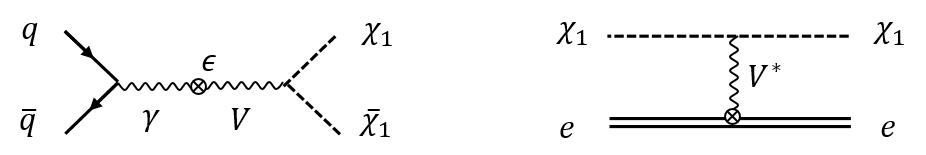
\includegraphics[width=\textwidth]{DM_prod_detect}
\caption[Direct production of \dword{dm} via the vector portal and \dword{dm}-electon elastic scattering]{\label{fig:dm_prod} Direct production of dark matter via the vector portal (left panel) and \dword{dm}-electon elastic scattering (right panel)}
\end{figure}
We are particularly interested in sub-GeV-range \dword{dm} coming from the decay of $on$-shell $V$ throughout this section. Therefore, the dominant production mechanism is the Drell-Yan process via dark photon $s$-channel exchange (see the left panel of Figure~\ref{fig:dm_prod}):

\begin{equation}
p + N \rightarrow V \rightarrow \chi_1 \bar \chi_1 \,.
\end{equation}
The cross section for production of the dark matter is then written as
\begin{equation}
\sigma(p + N \rightarrow V \rightarrow \chi_1 \bar \chi_1) = \sigma(pN\rightarrow V)\times {\rm Br}(V\rightarrow \chi_1 \bar \chi_1)\,.
\end{equation}
We can express the differential cross section as a function of the \dword{dm} laboratory-frame energy, $E_{\chi_1}$, and the angle
between its laboratory-frame momentum and the beam direction, $\theta$:
\begin{equation}
\frac{d\sigma(pN\rightarrow V\rightarrow \chi_1 \bar \chi_1)}{dE_{\chi_1}d\cos\theta} 
= \frac{\delta(x, \cos\theta)}{\delta(E_{\chi_1}, \cos\theta)}\cdot \frac{d\sigma(pN\rightarrow V)}{dx}\cdot {\rm Br}(V\rightarrow \chi_1 \bar{\chi}_1)\cdot g(\cos\theta),
\end{equation}
where the first factor on the right-hand side is the Jacobian associated with the above variable change. The
function $g$ describes the angular distribution of the \dword{dm} in the $V$ rest frame and $x$ is associated with parton distribution function (PDF).  This function %e parton distribution function (PDF) 
$f_{q/p(n)} (x)$ ) gives the probability of extracting the quark $q$ with momentum fraction $x$ from a
proton (neutron). See Ref.~\cite{deNiverville:2012ij} for detailed information about the PDF. \\
Once \dword{dm} is produced, %its detection can be done in 
the \dword{nd} can detect it by elastic electron scattering via \dword{nc} interactions, as depicted in the right panel of Figure~\ref{fig:dm_prod}.
The electron scattering differential cross section takes the form
\begin{equation}
\frac{d\sigma_{{\chi_1}e}}{dE_{e}} 
= 4\pi \epsilon^{2}\alpha_{11}\alpha \frac{2m_{e}E_{\chi_1}^{2} - (2m_{e}E_{\chi_1} + m_{\chi_1}^{2})(E_e-m_{e})}{(E_e^{2}-m_{\chi_1}^{2})(m_{V}^{2}+2m_{e}E_{e}-2m_{e}^{2})^{2}}\,,
\end{equation}
where $E_{e}$ is the electron recoil  energy, $E_{\chi_1}$ is the incoming \dword{dm} $\chi_1$ energy, and $\alpha_{11}$ is the fine structure constant between the dark photon and dark matter particles. 
A signal event involves only a recoil electron in the final state. Scattering angle and energy of such a scattered electron can be reconstructed in the \dword{nd}, so we consider these two kinematic observables as discriminators between our signal and various backgrounds.

\subsubsection{Background consideration}
 The background to the process shown in the right panel of Figure~\ref{fig:dm_prod} consists of any processes involving an electron recoil. As the \dword{nd} is located near the surface, background events, in general, can be induced by cosmic rays as well as by neutrinos generated from the beam. However, we do not consider the former possibility in this analysis because it is expected that a significant amount of cosmic background can be vetoed by the trigger and timing information of the injection beam. 
The major background will be neutrinos %stemming 
from the proton beam. 

We take $\nu$-electron %N.C. 
\dword{nc} events just for simplicity. 
Although an accurate data analysis requires  inclusion of all non-negligible background sources, in this ``preliminary'' study we %rather 
illustrate the overall flow of relevant procedures, leaving a more dedicated analysis for the future.
Nevertheless, we believe that our work here  not only gives guideline and some insights for future %actual 
analyses but also allows us to develop  intuition about the associated experimental sensitivities that DUNE %would 
might achieve.

\subsubsection{Simulation and event selection}
To generate event data of dark matter produced in the DUNE target, we
utilize the \texttt{MG5@aMC} particle event generation software~\cite{Alwall:2014hca}. 
For simplicity, we import 
the light dark matter model in eq.~\eqref{eq:lagrangian} for fermionic dark matter. We are only concerned with the direct production of dark matter via proton collision, and therefore analyze  the $p + p \rightarrow \chi_1 + \bar{\chi_1}$ process. 

    
    The next step in our calculations is to reweight the neutrino and dark
matter distributions so that they correspond to the correct number of \dword{pot} for the DUNE experiment. 

 \begin{figure}[!h]
 \centering
 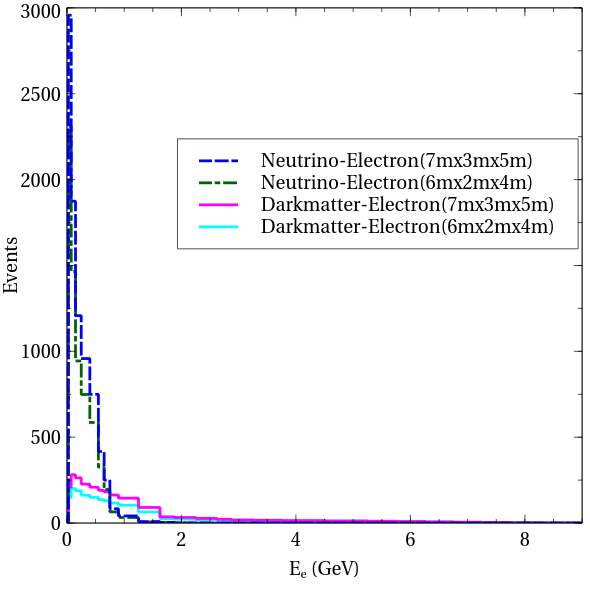
\includegraphics[width=8.0cm,height=5.8cm]{El_ScaEvent}
 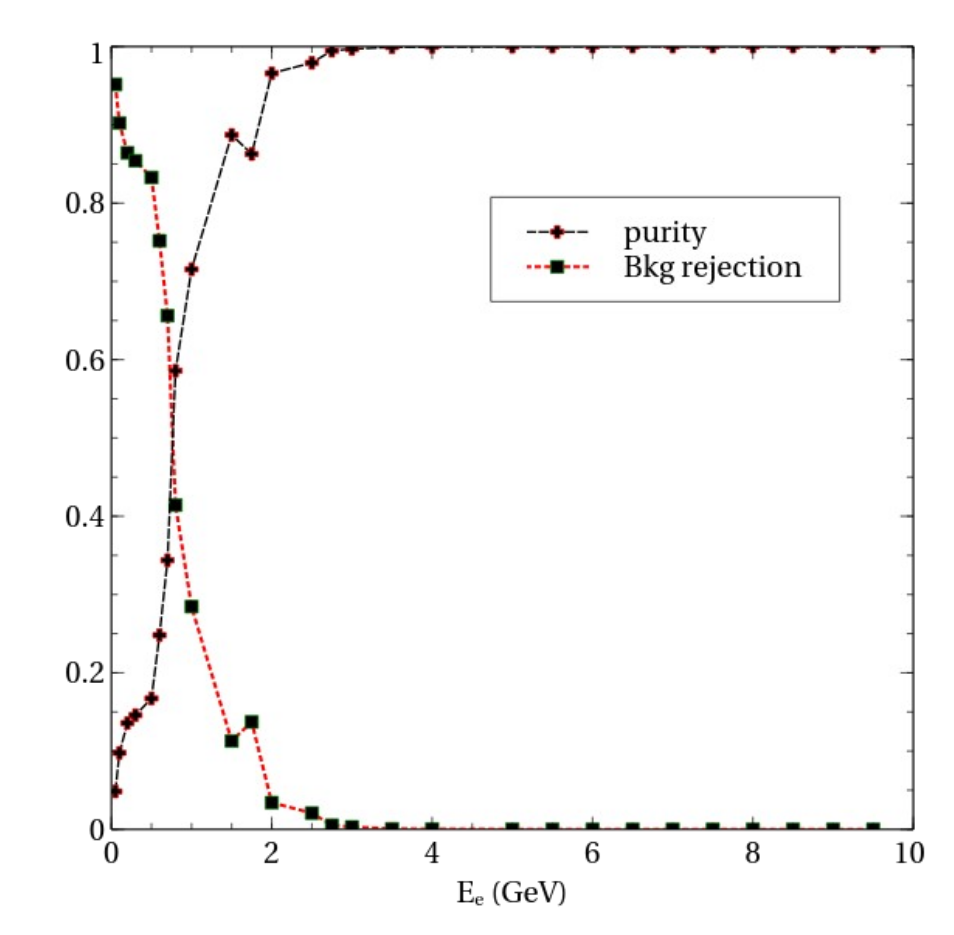
\includegraphics[width=8.0cm,height=6.0cm]{Purity}
 \caption[Scattered energy for two fiducial volumes and purities]{\label{fig:scatter_E} Scattered energy (left) for two different fiducial volumes and purities (right) shown for $m_{\chi_1}=2$ GeV, $m_{V}=6$ GeV, $\epsilon=10^{-3}$, and $\alpha_{11}=0.5$, respectively. }
 \end{figure}
 
The scattered energy distribution for both the signal and background events are shown in the left panel of Figure~\ref{fig:scatter_E}.
The background rate (i.e., $\nu$-electron scattered events) is very large at low energies (below $\sim\,1\,$GeV), whereas signal events display a harder spectrum. 
As mentioned earlier, \fixme{what section?} we have used two kinematic variables, the recoil energy and recoil angle, to reject background events. 
We introduce two dynamical variables as purity and background rejection for the event selection. 
Purity is defined as the ratio of the number of signal events over the total number of events for each energy and angular bin. 
Similarly, background rejection is defined as the ratio between number of background events over the total number of events. 
We calculate the sensitivity ($\chi^{2}$) for each energy and theta bin, and maximize the $\chi^{2}$ when the purity is greater or equal to background ratio (rejection). The right panel of Figure~\ref{fig:scatter_E} shows the purity and background rejection versus energy.

\subsubsection{Sensitivity calculation and results}
The sensitivity results for the analysis were generated for the dark sector parameters  $m_{V}=3m_{\chi_1}$, $\alpha_{11}=0.5$. 
We have calculated the $\chi^{2}$ sensitivity in the parameter space $Y$ vs $m_{\chi_1}$, where 
\begin{equation}
Y\equiv\epsilon^{2}\alpha_{11} (\frac{m_{\chi_1}}{m_{V}})^{4}
\end{equation}
is a dimensionless parameter that controls the \dword{dm} annihilation cross section and in turn the thermal relic abundance. 
For the $\chi^{2}$ calculation, we take into account smearing energy in the  \dword{nd}.
To smear energy, we use the predicted smearing of 5$\%$ presented in the DUNE \dword{cdr} \cite{Acciarri:2015uup} with a Gaussian resolution function.


The $\chi^{2}$ values are calculated for each set of two dark matter parameters ($Y$ vs $m_{\chi_1}$).
In Figure~\ref{fig:chisq}, with $m_{V} = 3m_{\chi}$ and $\alpha_{11}=0.5$,  the 90$\%$ C.L  values for the dimensionless \dword{dm} annihilation
cross section parameter $Y = \epsilon^{2}\alpha_{11} (m_{\chi}/m_{V})^4$ plotted for 120 GeV proton energy (left) compared to different experimental exclusion regions (right).
 \begin{figure}[t]
 \centering
 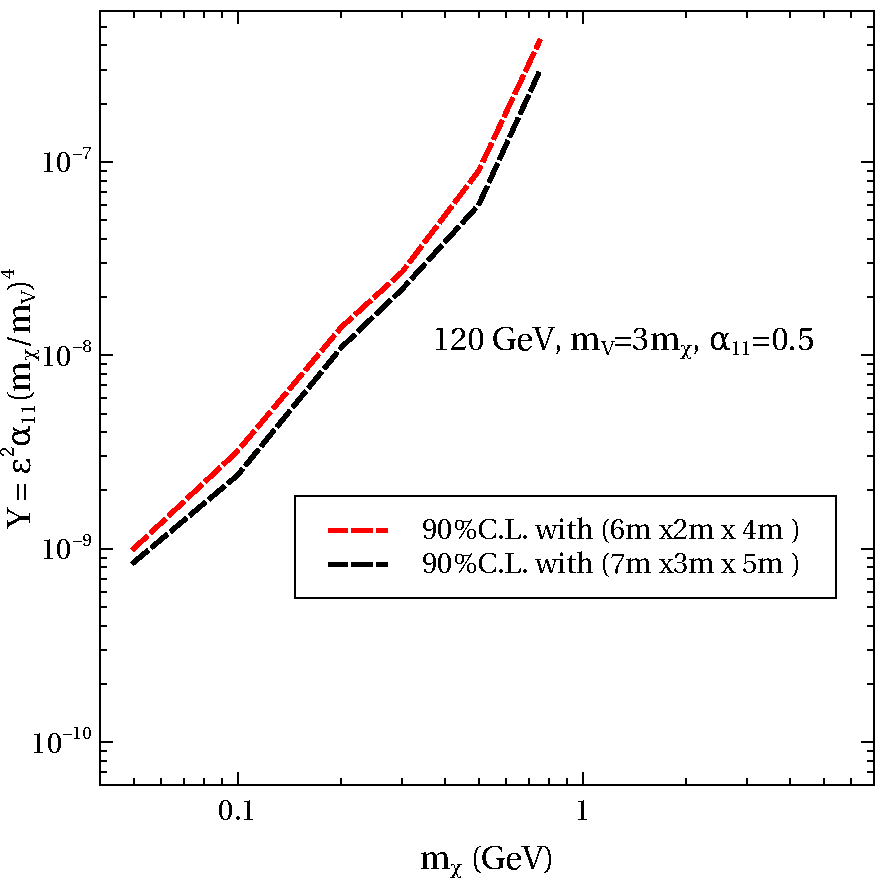
\includegraphics[width=7.5cm,height=5.8cm]{90CL_TDR}
 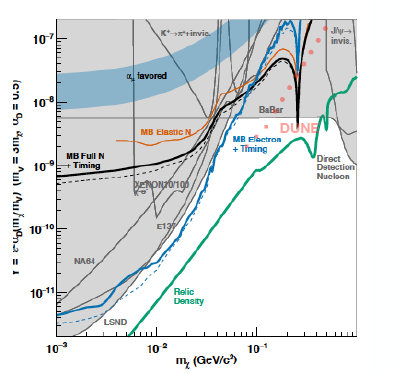
\includegraphics[width=8.0cm,height=6.0cm]{image2}
 \caption[90$\%$ Confidence level limit for Y as a function of $m_{\chi}$ at ND]{\label{fig:chisq} Left: 90$\%$ Confidence level limit for Y as a function of $m_{\chi}$, assuming $\alpha_{11}=0.5$ and $m_{V} = 3m_{\chi}$ at the DUNE \dword{nd}. 
The red dashed (black dashed) line shows the expected sensitivity for 120 GeV proton energy with \dword{nd} dimension  \SI{6}{m} $\times$ \SI{2}{m} $\times$ \SI{4}{m}  (\SI{7}{m} $\times$ \SI{3}{m} $\times$ \SI{5}{m}) fiducial volume. 
The chosen parameters are $\alpha_{11}=0.5$ and $m_{V}= 3m_{\chi_1}$.
Right: The sensitivity with the other experiments.}
 \end{figure}

%%%%%%%%%%%%%%%%%%%%%%%%%
\subsection{Cosmic Frontier Search: DUNE \dword{fd} and \dword{protodune} \label{sec:FD}}

\subsubsection{Flux of \dword{bdm} \label{sec:flux}}

As we mentioned in Section~\ref{phys:bsm:execsumm}, %the Introduction, 
we look at an annihilating two-component \dword{dm} scenario~\cite{Belanger:2011ww} in this study. 
The heavier \dword{dm} (denoted $\chi_0$) plays a role of cosmological \dword{dm} and pair-annihilates to a pair of lighter \dword{dm} particles (denoted $\chi_1$) in the universe today. 
The expected flux near the Earth is given by~\cite{Agashe:2014yua, Giudice:2017zke, Kim:2018veo}
\bea 
\mathcal{F}_1= & 1.6 \times 10^{-6} {\rm cm}^{-2}{\rm s}^{-1}\times \left( \frac{\langle \sigma v\rangle_{0\rightarrow 1}}{5\times 10^{-26}{\rm cm}^3{\rm s}^{-1}}\right) 
 \times \left( \frac{10\, {\rm GeV}}{m_{\chi_0}}\right)^2\,,
\label{eq:flux}
\eea
where $m_{\chi_0}$ is the mass of $\chi_0$ and $\langle \sigma v\rangle_{0\rightarrow 1}$ stands for the velocity-averaged annihilation cross section of $\chi_0\bar{\chi}_0 \to \chi_1\bar{\chi}_1$ in the current universe.
To evaluate the reference value shown as the first prefactor, we take $m_{\chi_0} = 10$ GeV and $\langle \sigma v\rangle_{0\rightarrow 1}=5\times 10^{-26}{\rm cm}^3{\rm s}^{-1}$, the latter of which is consistent with the current observation of \dword{dm} relic density assuming $\chi_0$ and its anti-particle $\bar{\chi}_0$ are distinguishable. 
To integrate all relevant contributions over the entire galaxy, we assume the Navarro-Frenk-White (NFW) \dword{dm} halo profile~\cite{Navarro:1995iw, Navarro:1996gj}.
In this section we assume the \dword{bdm} flux with a $m_{\chi_0}$ dependence given by eq.~(\ref{eq:flux}) for the phenomenological analysis. 


\subsubsection{Experimental signatures}

The \dword{bdm} that is created, e.g., at the galactic center, reaches the DUNE \dword{fd} and \dword{protodune} detectors and scatters off either electrons or protons energetically. 
In this study, we focus on electron scattering signatures for illustration. 
The overall process is summarized as follows:
\bea 
\chi_1 + e^- \to e^- + \chi_2 (\to \chi_1 + V^{(*)} \to \chi_1 + e^+ +e^-)\,,
\eea
and a diagrammatic description is shown in Figure~\ref{fig:sig} where %detector-visible 
particles visible by the detector are circled in blue. %enclosed by a blue circle. 
%Therefore, i
In the final state, there exist three visible particles that usually leave sizable ($e$-like) tracks in the %DUNE and \dword{protodune} 
detectors.  
Note that we can replace $e^-$ in the left-hand side and the first $e^-$ in the right-hand side of the above process to $p$ for the $p$-scattering case.
%In this case, the primary signature is quasi-elastic proton recoiling~\cite{pscattering} if the source of \dword{bdm} is the Galactic Center in the basic model in eq.~\eqref{eq:lagrangian}.
In the basic model, eq.~\eqref{eq:lagrangian}, and given the source of \dword{bdm} at the Galactic Center,  the primary signature is quasi-elastic proton recoiling~\cite{pscattering} in this case.

\begin{figure}[t]
\centering
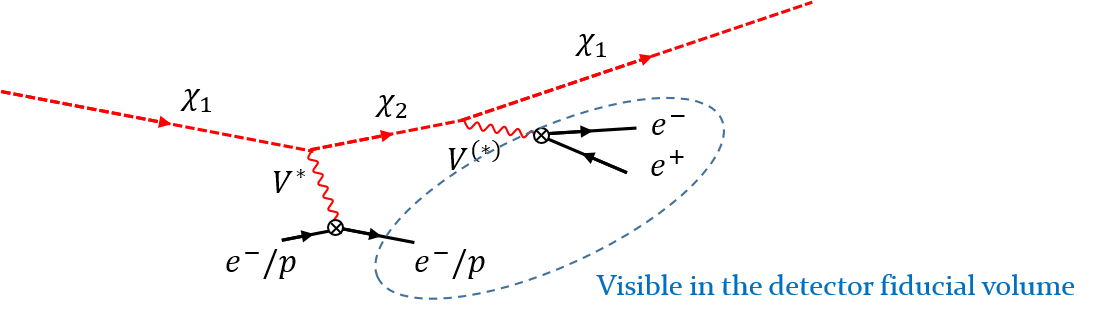
\includegraphics[width=6cm]{signature}
\caption{\label{fig:sig} The inelastic \dword{bdm} signal under consideration.}
\end{figure}

\subsubsection{Background estimation}

As we have identified a possible $i$\dword{bdm} signature, we are now in a position to discuss potential \dword{sm} background events. 

The biggest challenge in the search for \dword{bdm} signals at \dword{protodune} is the fact that it involves surface-based detectors, which suffer from an enormous amount of cosmic ray backgrounds such as muons or neutrons.
The most plausible scenario in which a cosmic muon might mimic the signal is as follows: a muon (1) enters the fiducial volume without leaving a track, i.e., ``sneaks-in'', (2) emits a hard photon which converts into an $e^+ e^-$ pair, and (3) starts to leave a visible track resulting in a signal-like event shape, (4) which appears electron-like.
For the criteria (1) and (4), we conservatively take the upper limits 0.1\% and 1\%, respectively, from some pre-existing dedicated studies of muon reconstruction efficiency under a similar LArTPC %-detector 
environment~\cite{MicroBooNEmuon, Acciarri:2016sli}.
If we achieve $\sim\,0.6\%$ of suppression power in criterion (3), the number of corresponding background events can be fewer than $\sim\,100$ per year at the \dword{protodune} detectors. \fixme{numbered things are not apples to apples. 4 is different.}


%When it comes to the 
For the DUNE \dwords{detmodule} located $\sim 1480$ m deep underground, the cosmic-induced background discussed earlier is not an issue. 
The most plausible scenario \fixme{for what, background production?} is the production of multiple pions that subsequently decay to electrons, positrons, and neutrinos. 
Relevant channels are the resonance production and/or \dword{dis} by the \dword{cc} $\nu_e$ or $\bar \nu_e$ scattering with a nucleon in the \lar target.
Summing up all the resonance production and \dword{dis} events that are not only induced by $\nu_e$ or $\bar \nu_e$ 
%whose energy is larger than 1 GeV, 
but relevant to production of a few pions, we find that the total number of multi-pion production events is at most $\sim 12$ kt$^{-1}$yr$^{-1}$ based on the neutrino flux in Ref.~\cite{Honda:2015fha} and the cross section in Ref.~\cite{Formaggio:2013kya}.
In addition, the charged pions often leave appreciable tracks inside the detector so that the probability of misidentifying the $e^\pm$ from the decays of $\pi^\pm$ with the \textit{i}\dword{bdm} signal events would be very small.
Hence, we conclude that it is fairly reasonable to assume that almost no background events exist.

For the \dword{protodune} detectors, each with fiducial mass $\sim0.5$ kt, the expected total number of atmospheric neutrino-induced multi-pion events is at most $\sim 6$ yr$^{-1}$, which would be significantly reduced again due to the good pion tagging efficiency. 
Thus, no atmospheric neutrino-induced backgrounds are expected for the \dword{protodune} detectors.  



\subsubsection{Phenomenology}\label{Sec:Pheno}

We finally present the expected experimental sensitivities at \dword{protodune} and DUNE, in the searches for $i$\dword{bdm}. 
We closely follow the strategies illustrated in Refs.~\cite{Giudice:2017zke, Chatterjee:2018mej, Kim:2018veo} to represent phenomenological interpretations. 

\begin{figure}[t]
\centering
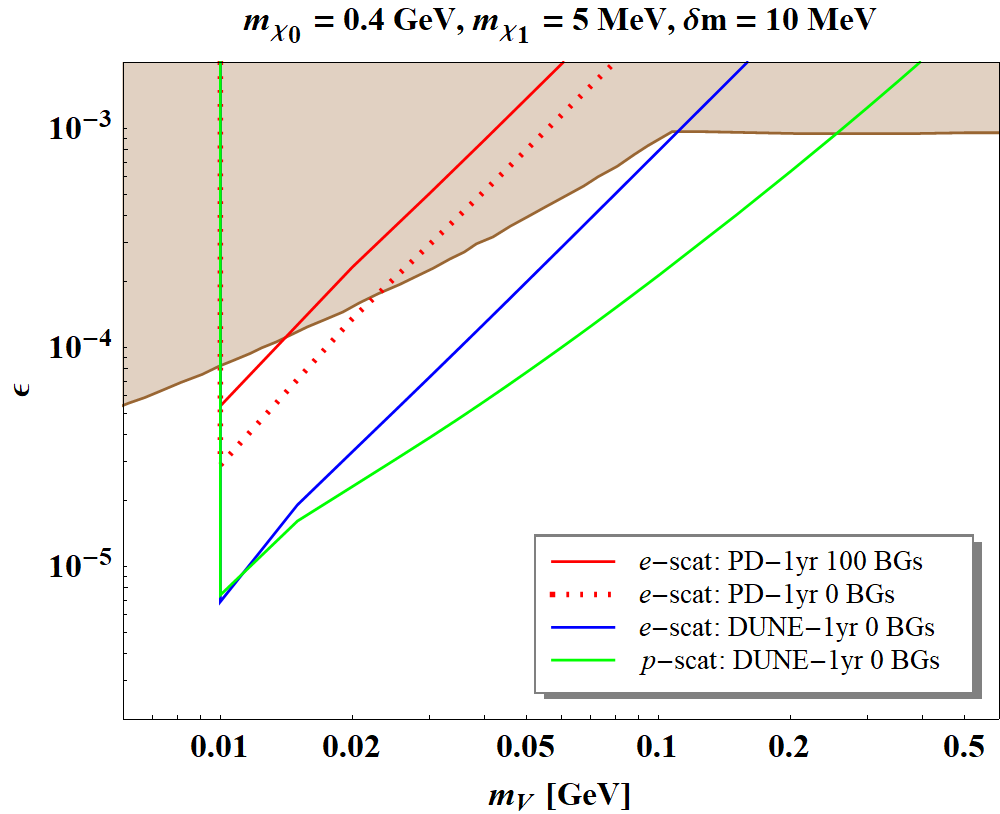
\includegraphics[width=6cm]{inv_PD_vs_DUNE} 
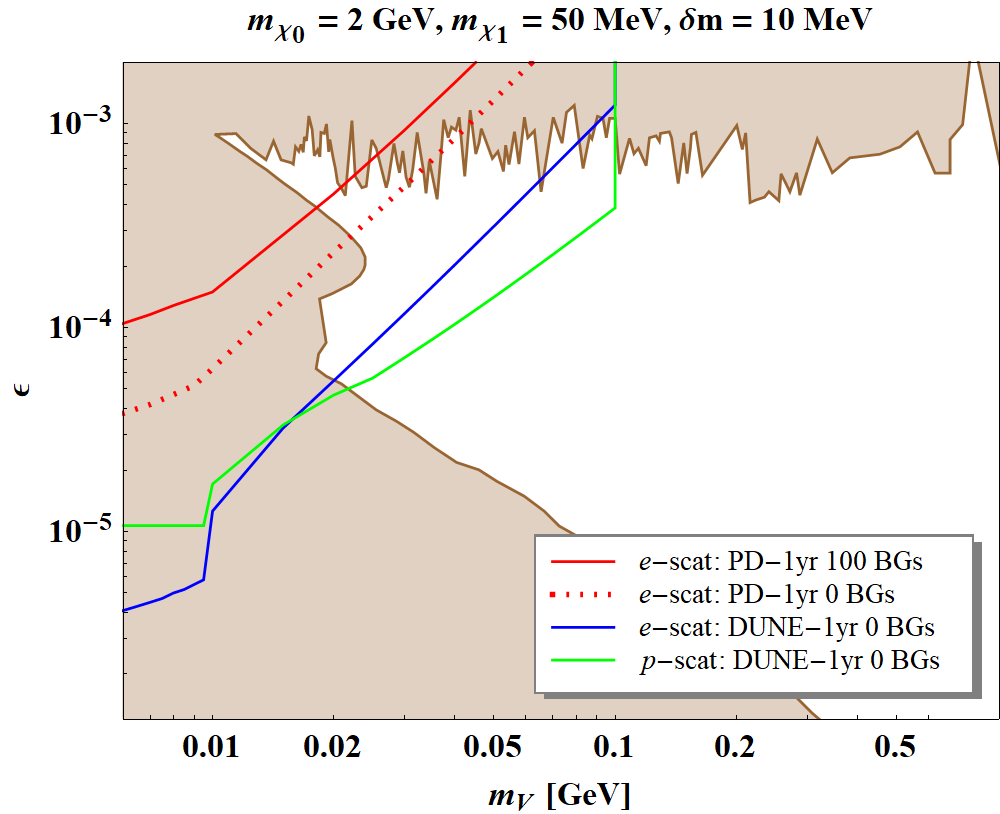
\includegraphics[width=6cm]{vis_PD_vs_DUNE} \\
\vspace{0.3cm}
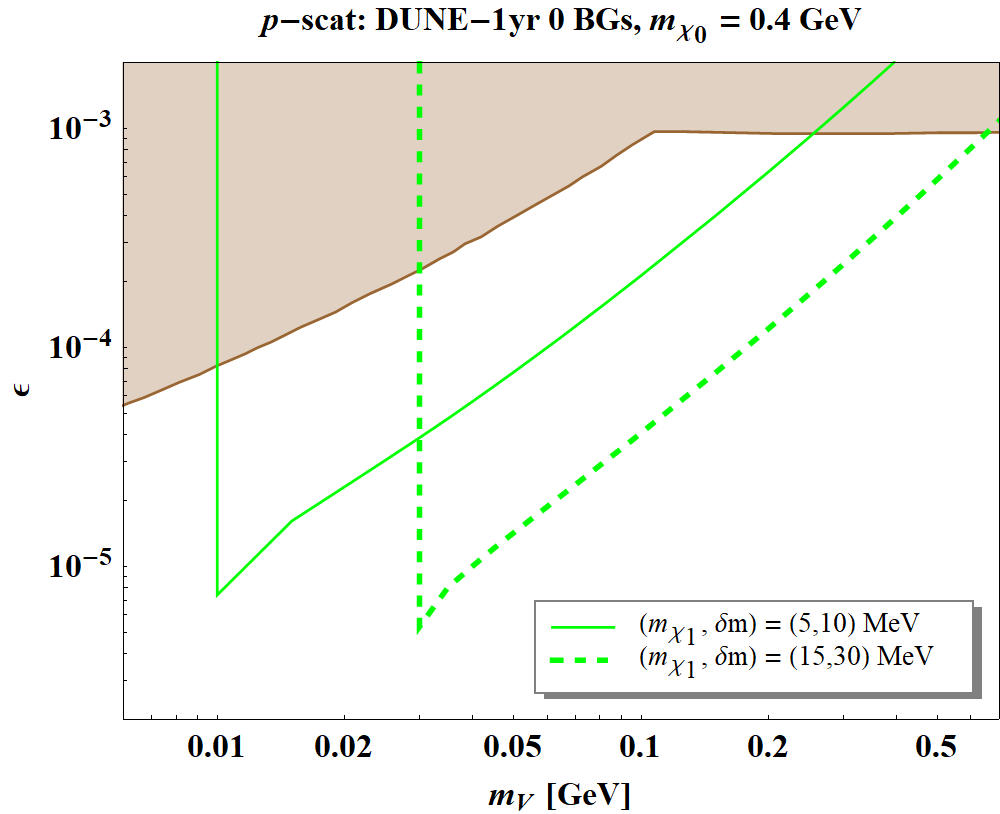
\includegraphics[width=6cm]{inv_DUNE_p-scatterings}
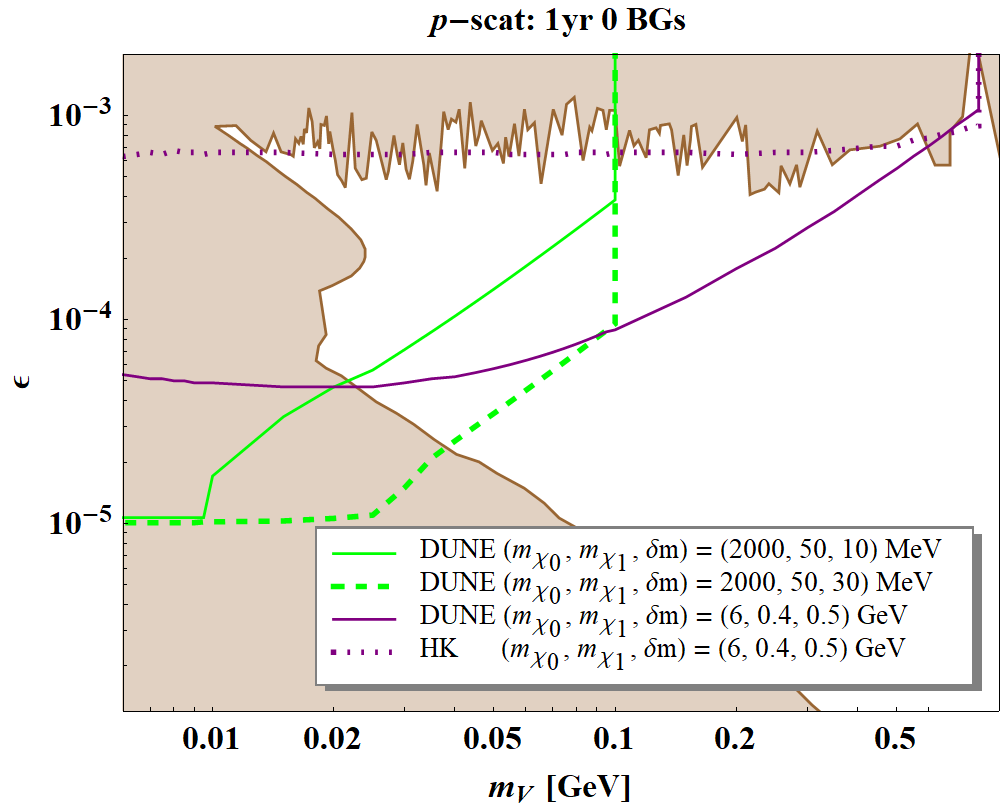
\includegraphics[width=6cm]{vis_DUNE_p-scatterings}
\caption[Experimental sensitivities for $m_{\chi_n}$ values in terms of $m_V - \epsilon$]{
The experimental sensitivities in terms of reference model parameters $m_V - \epsilon$ 
for $m_{\chi_0} = 0.4$ GeV, $m_{\chi_1} = 5$ MeV, and $\delta m = m_{\chi_2} - m_{\chi_1} = 10$ MeV (upper-left panel) and $m_{\chi_0} = 2$ GeV, $m_{\chi_1} = 50$ MeV, and $\delta m = 10$ MeV (upper-right panel).
The left panels are for Scenario 1 and the right ones are for Scenario 2.
The lower panels compare different reference points in the $p$-scattering channel.
See the text for the details.
\label{fig:darkphotonparameter} }
\end{figure}


In displaying the results, we separate the signal categories into %such that
%--
\begin{itemize}
\item Scenario 1: $m_V > 2 m_{\chi_1}$, experimental limits for $V \to$ invisible  applied.
\item Scenario 2: $m_V \le 2 m_{\chi_1}$, experimental limits for $V \to e^+ e^-$ invisible  applied.
\end{itemize}

The brown shaded region shows the latest limits set by various experiments such as the fixed target experiment NA64 at the CERN SPS and the B-factory experiment BaBar~\cite{Banerjee:2017hhz}.
The red solid (dotted) line describes the experimental sensitivity\footnote{This is defined as the boundary of parameter space that can be probed by the dedicated search in a given experiment at 90\% \dword{cl}, practically obtained from eq.~(\ref{eq:MIsensitivity}).} at \dword{protodune} under the assumption of 100 (zero) background events. 
The associated exposure is 470 t$\cdot$yr, i.e., a total fiducial volume of 470 t times 1-year running time. \fixme{t is metric ton? clarify}
The corresponding DUNE result is represented by the blue solid line with \fdfiducialmass $\cdot$ yr exposure and a zero background assumption. 
For comparison, we also show the sensitivities of DUNE to the $p$-scattering signal as a green solid line. 

Inspired by this potential of searching for the proton scattering channel, we study another reference parameter and compare it with the original one in the lower-left panel of Figure~\ref{fig:darkphotonparameter}. 
We see the reachable $\epsilon$ values rise, as $m_V$ increases. 


For Scenario 2 (the right panels of Figure~\ref{fig:darkphotonparameter}), we choose a different reference parameter set: $m_{\chi_0} = 2$ GeV, $m_{\chi_1} = 50$ MeV, $\delta m = 10$ MeV. 
The current limits (brown shaded regions), from various fixed target experiments, B-factory experiments, and astrophysical observations, are taken from Ref.~\cite{Banerjee:2018vgk}.


We next discuss model-independent experimental sensitivities. 
The experimental sensitivities are determined by the number of signal events excluded at 90\% \dword{cl} in the absence of an observed signal.
The expected number of signal events, $N_{\rm sig}$, is given by
\begin{align}
N_{\rm sig} = \sigma_\epsilon \mathcal F A(\ell_{\rm lab}) t_{\rm exp} N_T\,,
\label{eq:NS}
\end{align}
where $T$ stands for the target that $\chi_1$ scatters off, $\sigma_\epsilon$ is the cross section of the primary scattering $\chi_1 T \to \chi_2 T$, $\mathcal F$ is the flux of $\chi_1$, $t_{\rm exp}$ is the exposure time, and $A(\ell_{\rm lab})$ is the acceptance that is defined as 1 if the event occurs within the fiducial volume and 0 otherwise.
Here we determine the acceptance for an $i$\dword{bdm} signal by the distance between the primary and secondary vertices in the laboratory frame, $\ell_{\rm lab}$, so $A(\ell_{\rm lab}) = 1$ when both the primary and secondary events occur inside the fiducial volume. (Given this definition, obviously, $A(\ell_{\rm lab}) = 1$ for elastic \dword{bdm}.)
%Note that o
Our notation $\sigma_\epsilon$ includes additional realistic effects from cuts, threshold energy, and the detector response, hence it can be understood as the fiducial cross section.

The 90\% \dword{cl} exclusion limit, $N_s^{90}$, can be obtained with a modified frequentist construction~\cite{cls1,cls2}. We follow the methods in Refs.~\cite{Dermisek:2013cxa,Dermisek:2014qca,Dermisek:2016via} in which the Poisson likelihood is assumed. 
An experiment becomes sensitive to the signal model independently if $N_{\rm sig} \ge N_s^{90}$.
Plugging eq.~\eqref{eq:NS} here, we find the experimental sensitivity expressed by %the following inequality
\begin{align}
\sigma_\epsilon \mathcal F \ge \frac{N_s^{90}}{A(\ell_{\rm lab}) t_{\rm exp} N_T}\,. 
\label{eq:MIsensitivity}
\end{align}
Since $\ell_{\rm lab}$ differs event-by-event, we take the maximally possible value of laboratory-frame mean decay length, i.e., $\bar{\ell}_{\rm lab}^{\rm max} \equiv \gamma_{\chi_2}^{\max} \bar{\ell}_{\rm rest}$ where $\gamma_{\chi_2}^{\max}$ is the maximum boost factor of $\chi_2$ and $\bar{\ell}_{\rm rest}$ is the rest-frame mean decay length. 
We emphasize that this is a rather conservative approach, because the acceptance $A$ is inversely proportional to $\ell_{\rm lab}$.
We then show the experimental sensitivity of any kind of experiment for a given background expectation, exposure time, and number of targets, in the plane of $\bar{\ell}_{\rm lab}^{\rm max} - \sigma_\epsilon \cdot \mathcal F$. 
The left panel of Figure~\ref{fig:modelindependent} demonstrates the expected model-independent sensitivities at several experiments. 
The red (orange) line is for the \dword{protodune} detectors with the assumptions of 100 (zero) background events and 470 t$\cdot$yr exposure, while the green (blue) is for the DUNE \dword{fd} with a background-free assumption and 20 (40) kt$\cdot$yr exposure.

\begin{figure}[t]
\centering
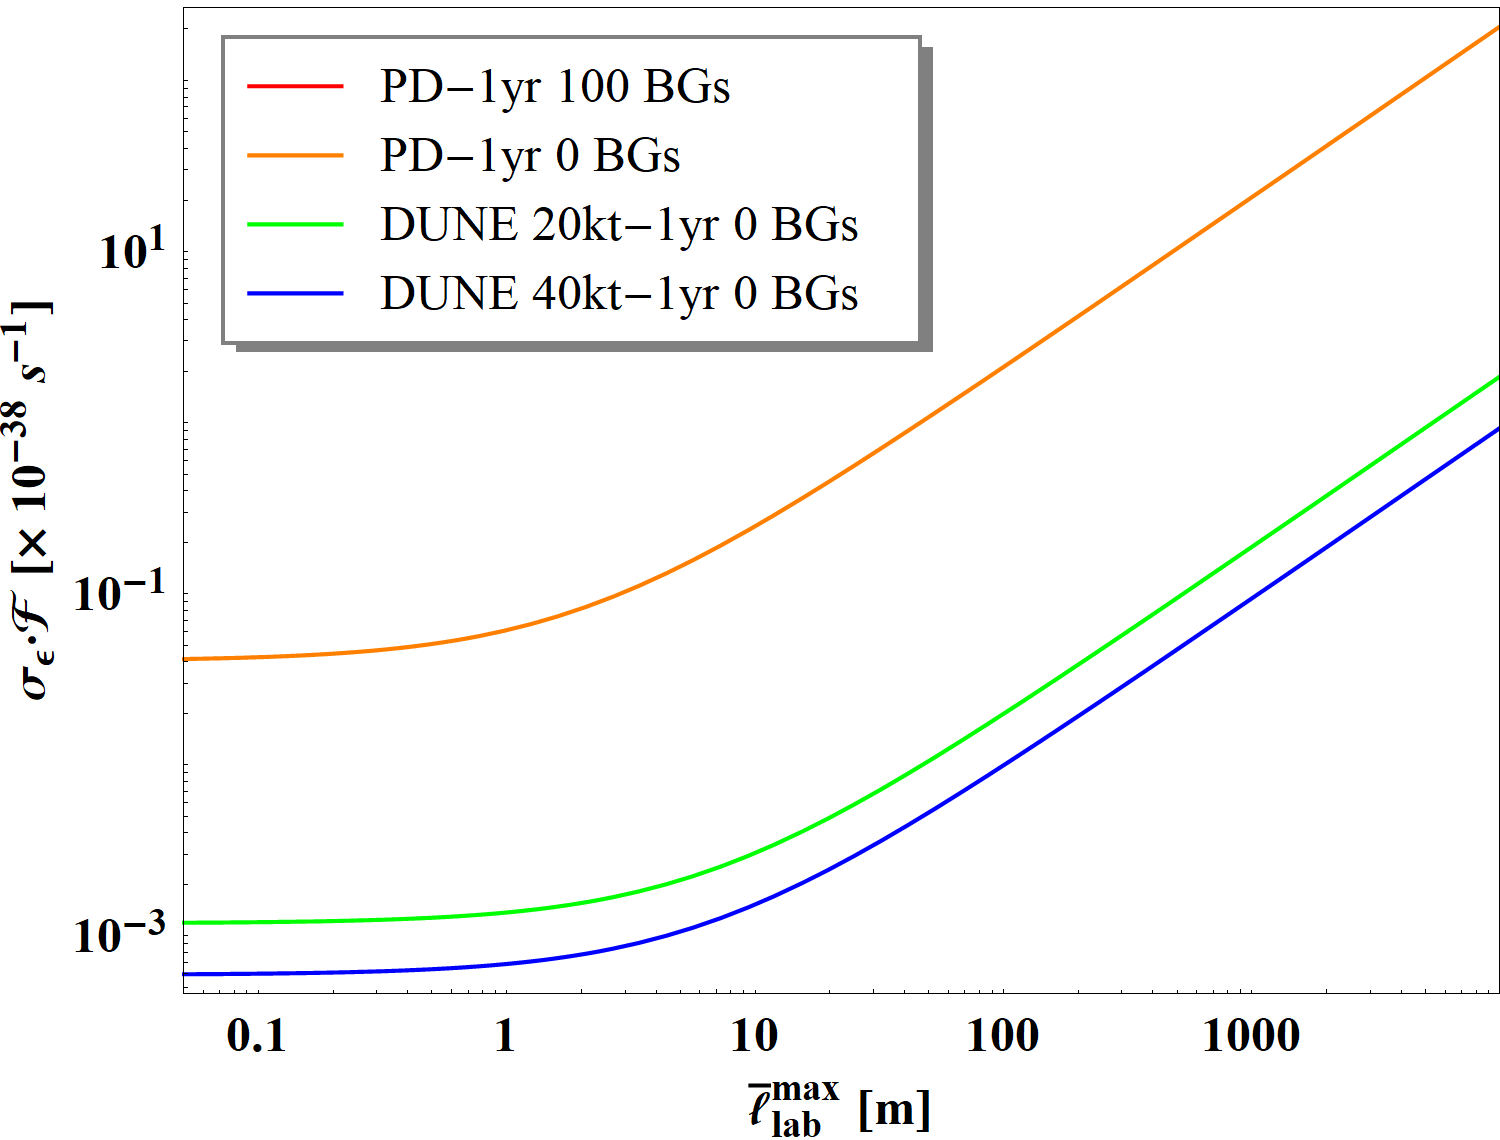
\includegraphics[width=6cm]{SigmaFluxVslMaxLab_TotalOnly}
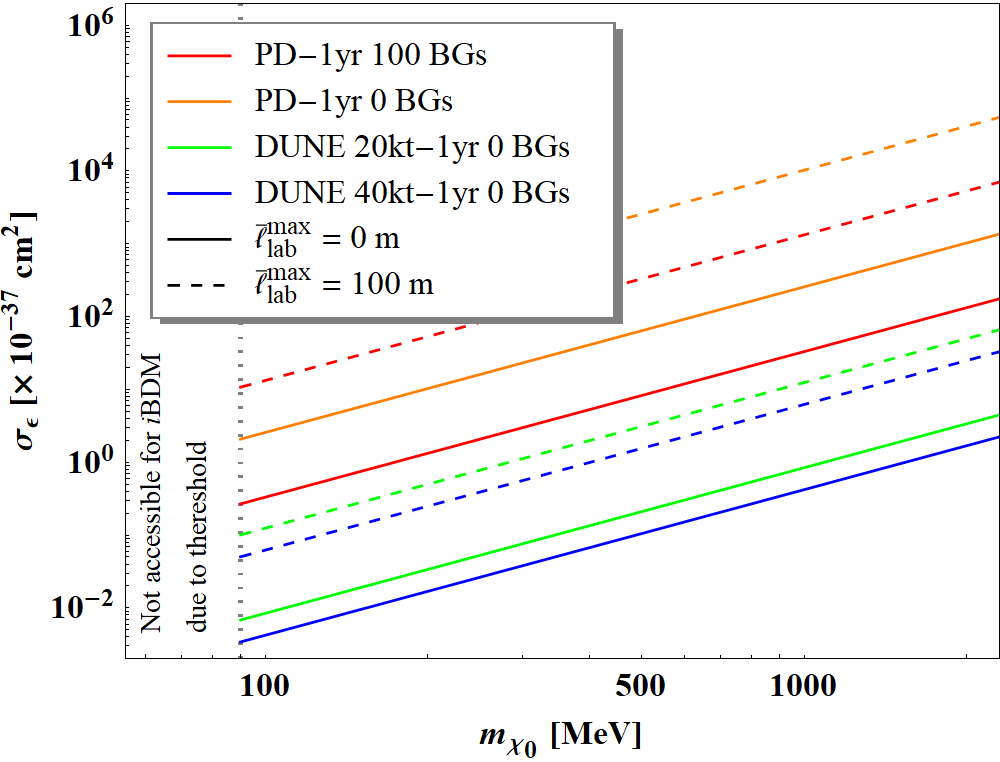
\includegraphics[width=6cm]{SigmaVsE1}
\caption[Model-independent experimental sensitivities of $i$\dword{bdm} search]{
Left: model-independent experimental sensitivities of $i$\dword{bdm} search in $\bar{\ell}_{\rm lab}^{\rm max} - \sigma_\epsilon \cdot \mathcal F$ plane. 
The reference experiments are \dword{protodune} with 100 background (red), zero-background (orange) assumption for 1-year time exposure, DUNE 20kt (green), and DUNE 40kt (blue) with zero-background assumption for 1-year time exposure. 
Right: Experimental sensitivities of $i$\dword{bdm} search in $m_{\chi_0} - \sigma_\epsilon$ plane. The sensitivities for $\bar{\ell}_{\rm lab}^{\rm max} = 0$ m and 100 m are shown as solid and dashed lines for each reference experiment in the left panel.
\label{fig:modelindependent} }
\end{figure}

The right panel of Figure~\ref{fig:modelindependent} reports model-dependent sensitivities for $\bar{\ell}_{\rm lab}^{\rm max} = 0$ m and 100 m corresponding to the experiments in the left panel.
Note that this %way 
method of presentation is reminiscent of the widely known scheme for showing the experimental reaches in various \dword{dm} direct detection experiments, i.e., $m_{\rm DM} - \sigma_{\rm DM - target}$ where $m_{\rm DM}$ is the mass of \dword{dm} and $\sigma_{\rm DM - target}$ is the cross section between the \dword{dm} and target. 
For the case of non-relativistic \dword{dm} scattering in the direct-detection experiments, $m_{\rm DM}$ determines the kinetic energy scale of the incoming \dword{dm}, just like $m_{\chi_0}$ sets out the incoming energy of boosted $\chi_1$ in the $i$\dword{bdm} search. 

%%%%%%%%%%%%%%%%%%%%%%%%%
\subsection{Discussions and Conclusions}

In this work, we have conducted simulation studies of the light dark matter model described in eq.~\eqref{eq:lagrangian} in terms of their detection prospects at the DUNE \dword{nd} and \dword{fd}. 

In the case of the \dword{nd}, we assumed that the relativistic \dword{dm} is being produced directly at the target (i.e., intensity-frontier approach) and leaves an experimental signature through an elastic electron scattering. Using two constrained parameters of the light \dword{dm} model and a range of two free parameters, a sensitivity map was produced. Within the context of the vector portal \dword{dm} model and the chosen parameter constraints along with the electron scattering as the signal event, this result sets the stringent limits on \dword{dm} parameters that are comparable or even better than recent experimental bounds in the sub-GeV mass range.

By contrast, in the case of the \dword{fd} modules, we assumed that the signal events are due to \dword{dm} coming from the galactic halo (i.e., cosmic-frontier approach) with a significant boost factor. The \dword{dm} scatters off either an electron or proton in the detector material into a heavier unstable dark-sector state (i.e., \textit{in}elastic scattering). 
The heavier state, by construction, decays back to \dword{dm} and an electron-positron pair via a dark-photon exchange. 
Therefore, in the final state, a signal event comes with an electron or proton recoil plus an electron-positron pair. 
This distinctive signal feature enabled us to perform (almost) background-free analyses. 
As \dword{protodune} detectors are prototypes of DUNE \dword{fd} modules, the same study was conducted and corresponding results were compared with the ones of the DUNE \dword{fd} modules.  
We first investigated the experimental sensitivity in a dark-photon parameter space, dark-photon mass $m_V$ versus kinetic mixing parameter $\epsilon$. 
The results were shown separately for Scenario 1 and 2. 
They suggest that \dword{protodune} and DUNE \dword{fd} modules would probe a broad range of unexplored regions; they would allow for reaching $\sim 1-2$ orders of magnitude smaller $\epsilon$ values than the current limits along MeV to sub-GeV-range dark photons. 
We also examined model-independent reaches at both \dword{protodune} detectors and DUNE \dword{fd} modules, providing limits for models conceiving $i$\dword{bdm} (or $i$\dword{bdm}-like) signals (i.e., a target recoil and a fermion pair). 
\fixme{models `conceiving' these things? models that assume the existence of?}



%%%%%%%%%%%%%%%%%%%%%%%%%%%%%%%%%%%%%%%%
\section{Sterile Neutrino Searches}
Experimental results in tension with the three-neutrino-flavor paradigm~\cite{LSNDSterile,MiniBooNESterile,GalliumSummary,ReactorSummary}, which may be interpreted as mixing between the known active neutrinos and one or more \textit{sterile} states, have led to a rich and diverse program of searches for oscillations into sterile neutrinos. Having a longer baseline, a more intense beam, and a high-resolution large-mass \dword{fd}, %when 
compared to previous experiments, DUNE provides a unique opportunity to improve significantly on the sensitivities of existing probes, and to enhance the ability to map the extended parameter space if a sterile neutrino is discovered.
	
%%%%%%%%%%%%%%%%%%%%%%%%%
\subsection{Probing Sterile Neutrino Mixing with DUNE}

    Long-baseline experiments like DUNE can look for sterile neutrino oscillations by measuring disappearance of the beam neutrino flux between the \dword{nd} and \dword{fd}. This results from the quadratic suppression of the sterile mixing angle measured in appearance experiments, $\theta_{\mu e}$, with respect to its disappearance counterparts, $\theta_{\mu\mu}\approx\theta_{24}$ for \dword{lbl} experiments, and $\theta_{ee}\approx\theta_{14}$ for reactor experiments. These disappearance effects have not yet been observed and are in tension with appearance results~\cite{ref:tension} when global fits of all available data are carried out. %Due to 
    Its high-intensity and high-resolution \dword{fd} will allow DUNE %will also be able 
    to perform direct measurements of nonstandard electron (anti)neutrino disappearance. 

DUNE will look for active-to-sterile neutrino mixing using the reconstructed energy spectra of both \dword{nc}  and \dword{cc}  neutrino interactions  in the \dword{fd}, and their comparison to the extrapolated predictions from the \dword{nd} measurement. Since \dword{nc} cross sections and interaction topologies are the same for all three active neutrino flavors, the \dword{nc} spectrum is insensitive to standard neutrino mixing. However, should there be oscillations into a fourth light neutrino, an energy-dependent depletion of the neutrino flux would be observed at the \dword{fd}, as the sterile neutrino would not interact in the detector volume. Furthermore, if sterile neutrino mixing is driven by a large mass-square difference $\Delta m^2_{\rm{41}}$ $\sim$1\,eV$^{2}$, the \dword{cc} spectrum will be distorted at energies higher than the energy corresponding to the standard oscillation maximum. Therefore, \dword{cc} disappearance is also a powerful probe of sterile neutrino mixing at long baselines. 

At long baselines, the \dword{nc} disappearance probability to first order in small mixing angles is given by:
\begin{equation}
\begin{aligned}
1 - P(\nu_{\mu} \rightarrow \nu_s) & \approx 1 - \cos^4\theta_{14}\cos^2\theta_{34}\sin^{2}2\theta_{24}\sin^2\Delta_{41} \\
& - \sin^2\theta_{34}\sin^22\theta_{23}\sin^2\Delta_{31} \\
& + \frac{1}{2}\sin\delta_{24}\sin\theta_{24}\sin2\theta_{23}\sin\Delta_{31},
\end{aligned}
\end{equation}
where $\Delta_{ji} = \frac{\Delta m^2_{ji}L}{4E}$. 
The relevant oscillation probability for \numu~\dword{cc} disappearance is the \numu~survival probability, similarly approximated by:
\begin{equation}
\begin{aligned}
P(\nu_{\mu} \rightarrow \nu_{\mu}) &\approx 1 - \sin^22\theta_{23}\sin^2\Delta_{31} \\
& + 2\sin^22\theta_{23}\sin^2\theta_{24}\sin^2\Delta_{31} \\ 
& - \sin^22\theta_{24}\sin^2\Delta_{41}.
\label{eq:NuMuDisFull}
\end{aligned}
\end{equation}
Finally, the disappearance of $\overset{(-)}\nu\!\!_e$~\dword{cc} is described by: 
\begin{equation}
\begin{aligned}
P(\overset{(-)}\nu\!\!_e \rightarrow \overset{(-)}\nu\!\!_e) &\approx 1 - \sin^22\theta_{13}\sin^2\Delta_{31} \\
& - \sin^22\theta_{14}\sin^2\Delta_{41}.
\label{eq:NueDisFull}
\end{aligned}
\end{equation}

Figure~\ref{fig:regimes} shows how the standard three-flavor oscillation probability is distorted at neutrino energies above the standard oscillation peak when oscillations into sterile neutrinos are included.
\begin{figure}[!h]
	\vspace{0pt}
	\begin{center}
	  	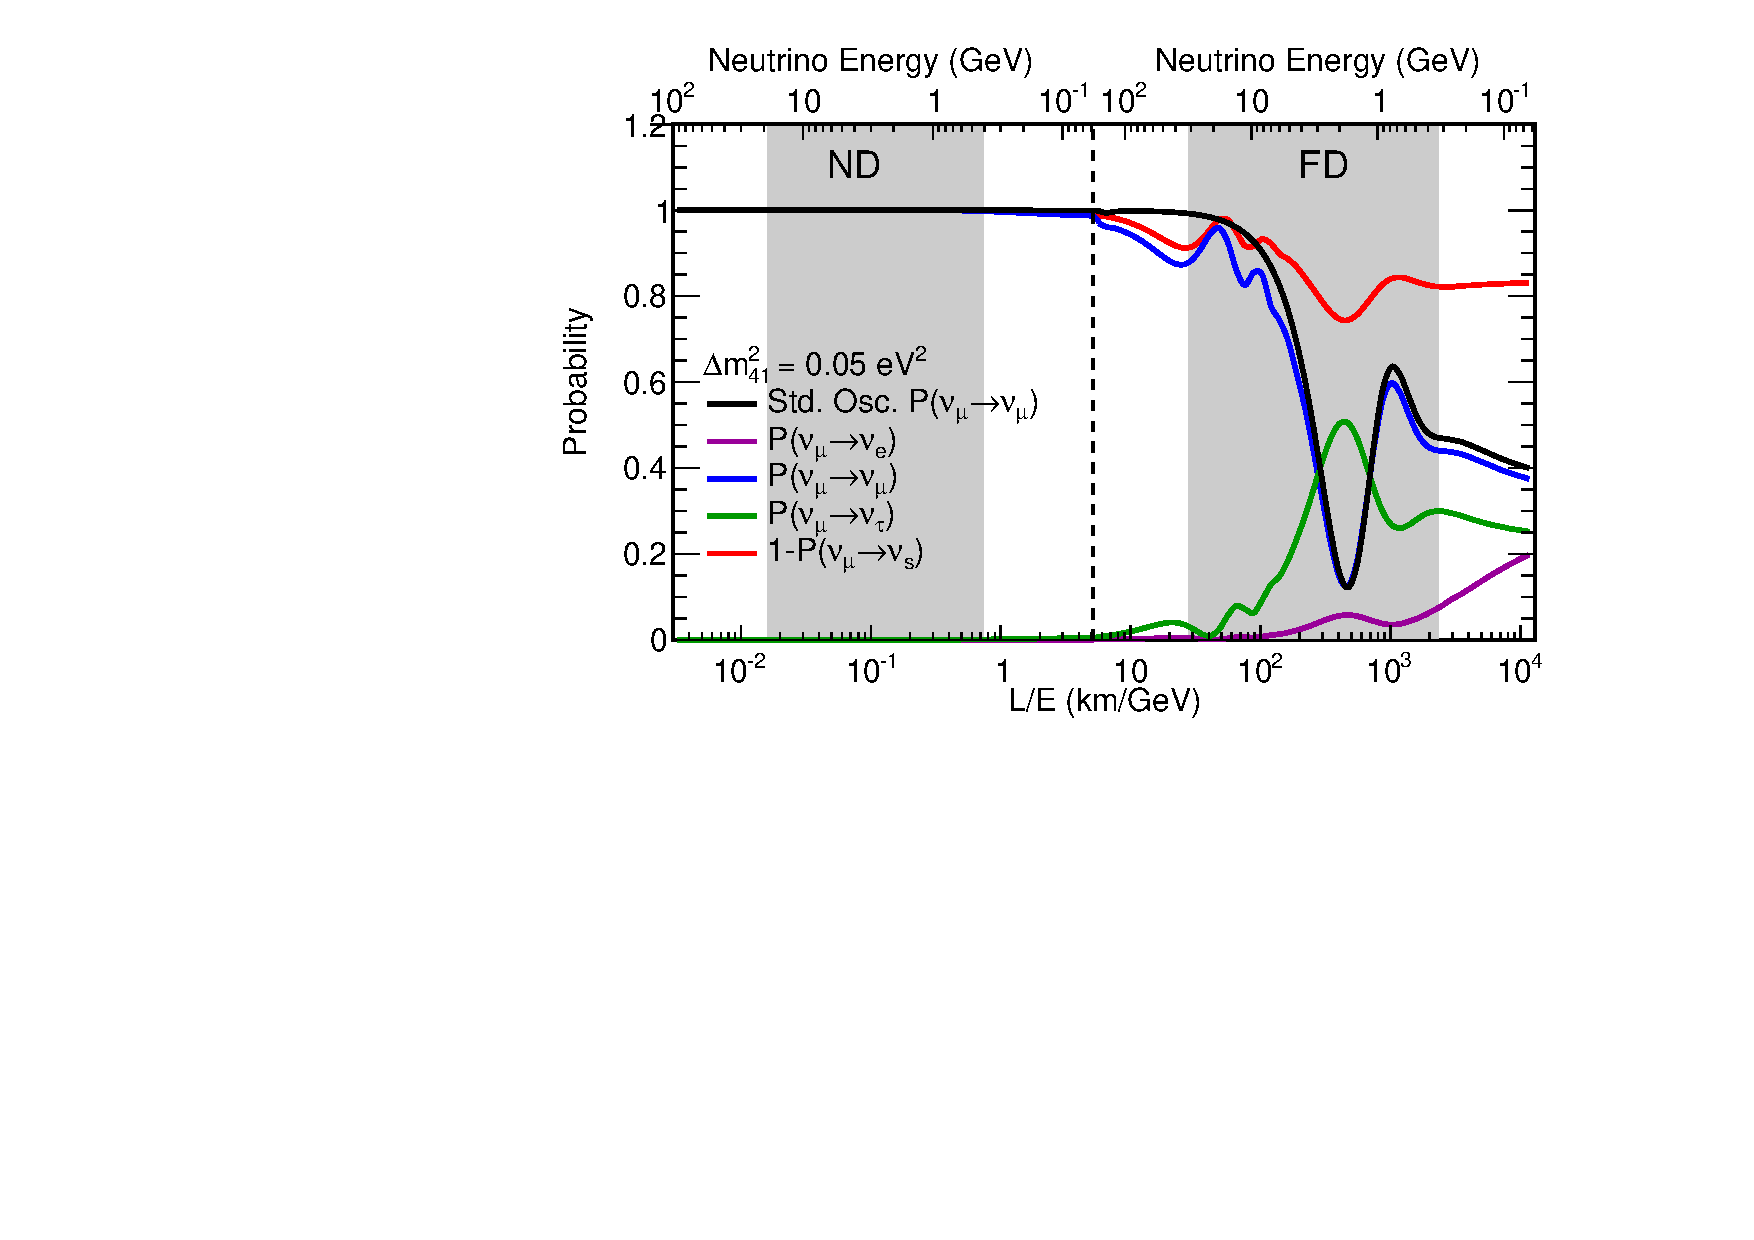
\includegraphics[width=0.49\textwidth]{DUNE_SterileSensi_dm0_05.pdf}
        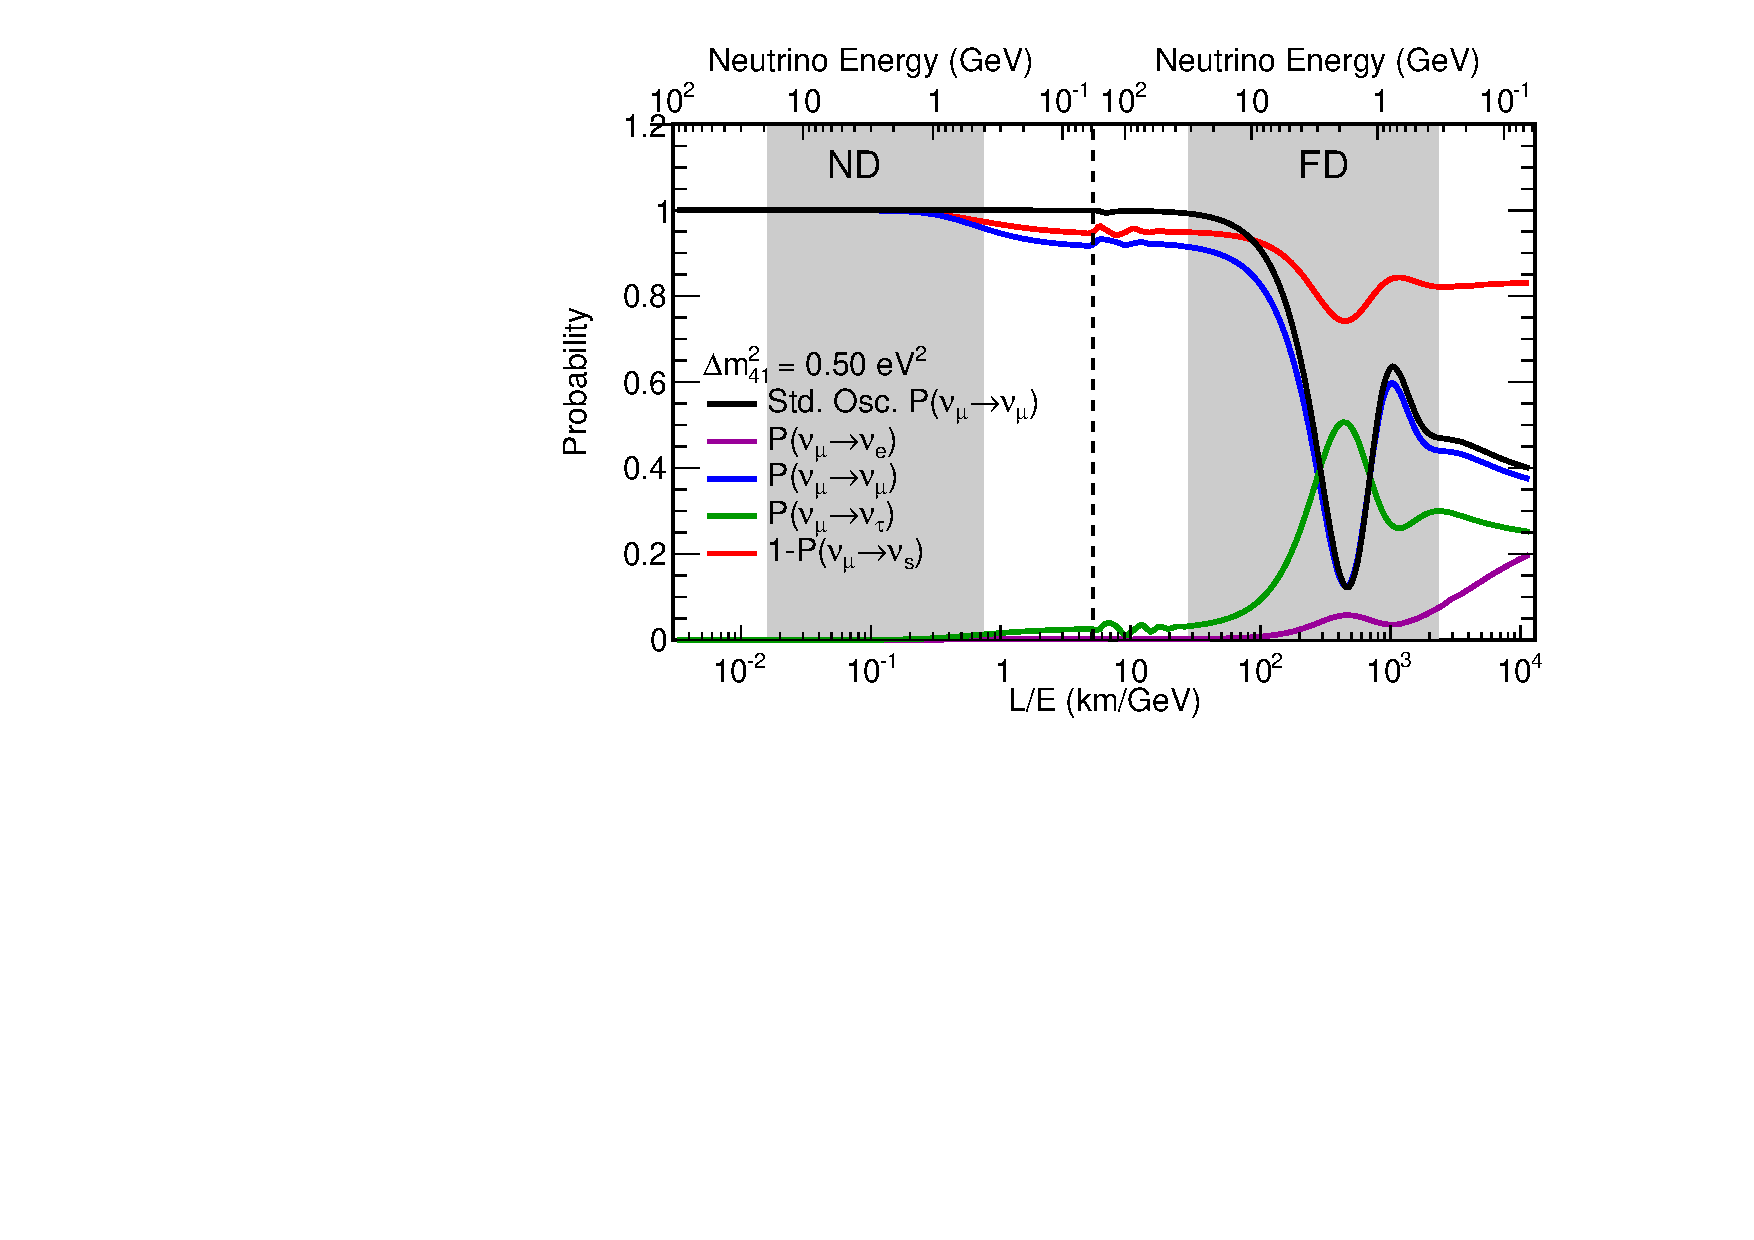
\includegraphics[width=0.49\textwidth]{DUNE_SterileSensi_dm0_5.pdf}
        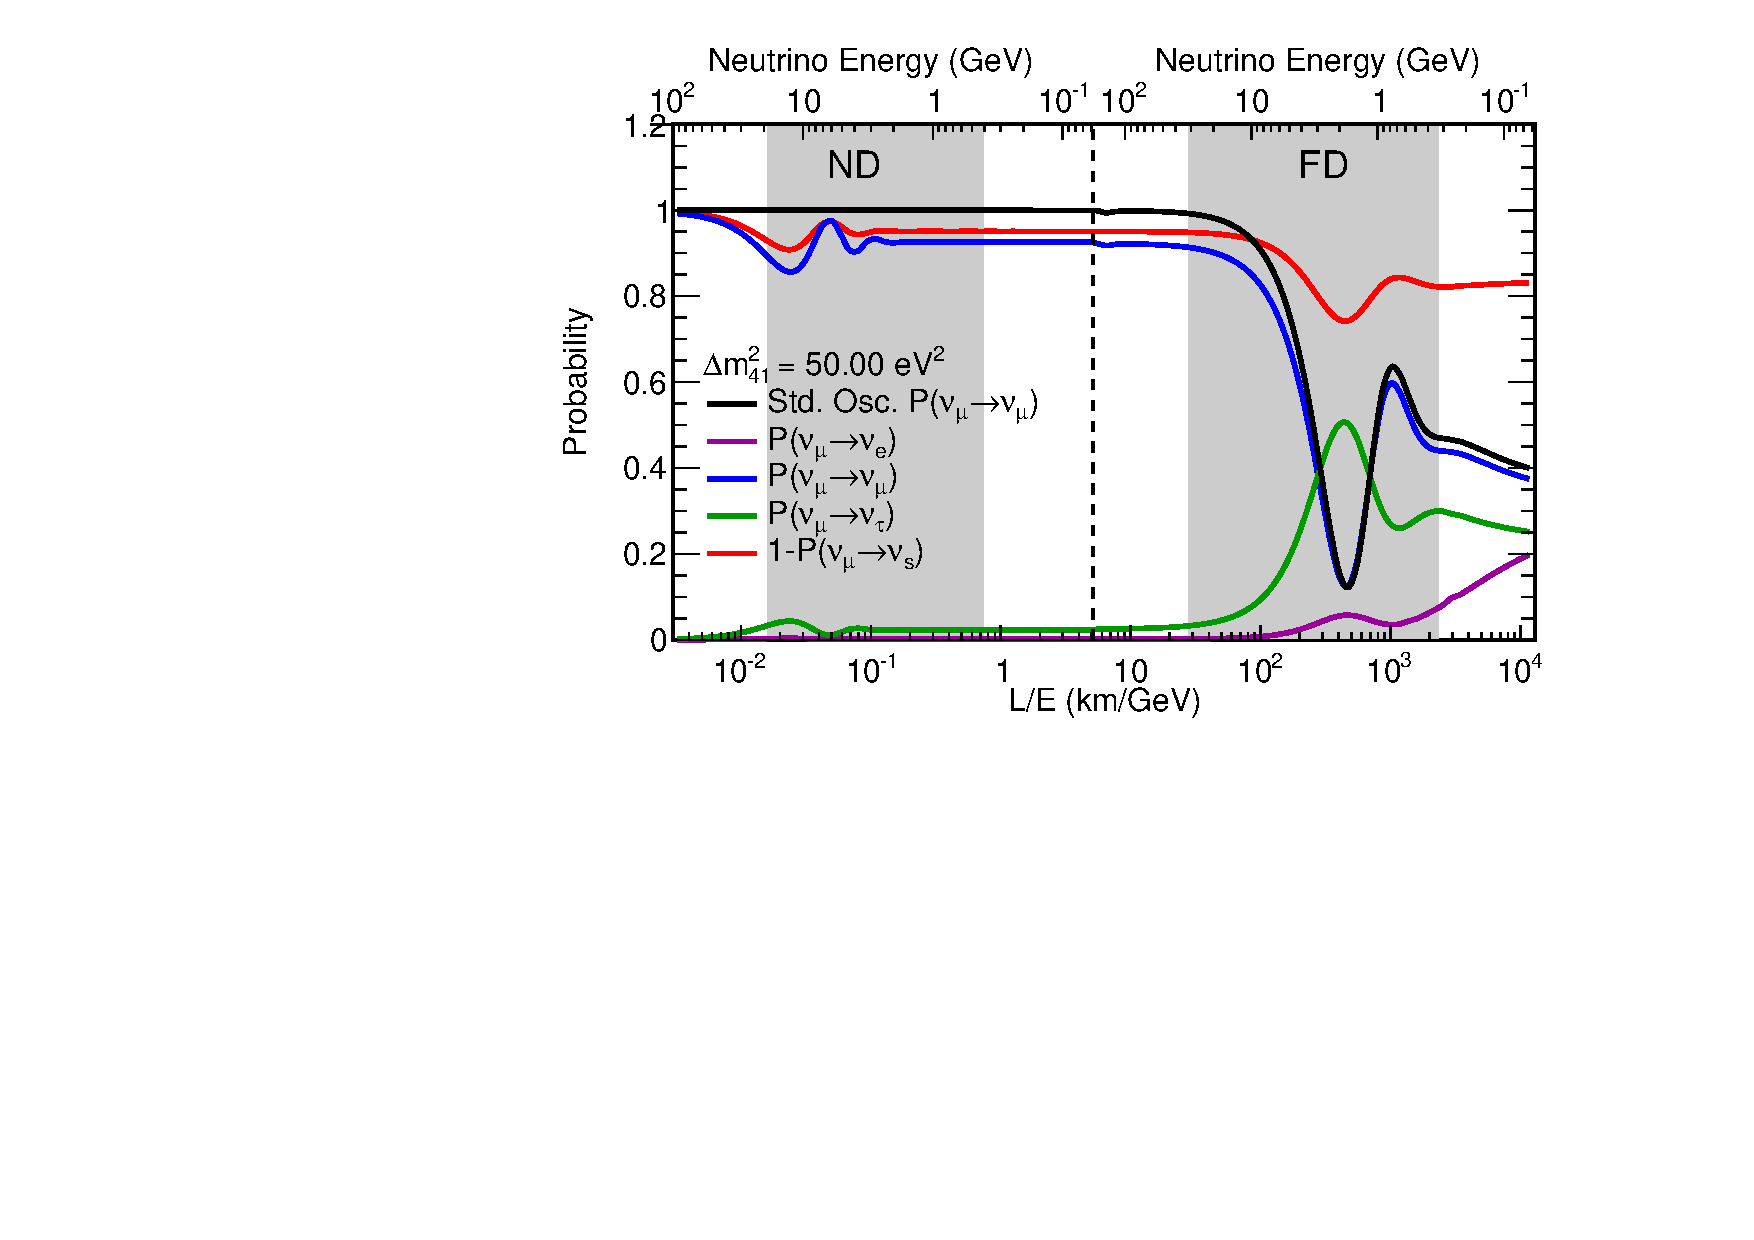
\includegraphics[width=0.49\textwidth]{DUNE_SterileSensi_dm50.pdf}
	\end{center}
\vspace{0pt}
\caption[Regions of $L/E$ probed by DUNE compared to 3-flavor and 3+1-flavor $\nu$ (dis)appearance probabilities]{Regions of $L/E$ probed by the DUNE detector compared to 3-flavor and 3+1-flavor neutrino disappearance and appearance probabilities. The gray-shaded areas show the range of true neutrino energies probed by the \dword{nd} and \dword{fd}. The top axis shows true neutrino energy, increasing from right to left. The top-left plot shows the probabilities assuming mixing with one sterile neutrino with $\Delta m^2_{\rm{41}}=0.05$~eV$^2$, corresponding to the slow oscillations regime. The top-right plot assumes mixing with one sterile neutrino with $\Delta m^2_{\rm{41}}=0.5$~eV$^2$, corresponding to the intermediate oscillations regime. The bottom plot includes mixing with one sterile neutrino with $\Delta m^2_{\rm{41}}=50$~eV$^2$, corresponding to the rapid oscillations regime. As an example, the slow sterile oscillations cause visible distortions in the three-flavor \numu~survival probability (blue curve) for neutrino energies $\sim10$\,GeV, well above the three-flavor oscillation minimum.}
  \label{fig:regimes}
 \vspace{0pt}
\end{figure}

%%%%%%%%%%%%%%%%%%%%%%%%%
\subsection{Setup and Methods}
The simulation of the DUNE experimental setup was performed with the  \dword{globes} software~\cite{Huber:2004ka,Huber:2007ji} using the DUNE \dword{cdr} configuration presented in Ref.~\cite{Alion:2016uaj} as a starting point. The sterile neutrino effects have been implemented in  \dword{globes} via the existing plug-in for sterile neutrinos and \dword{nsi}~\cite{Joachim}. As described above, the \dword{nd} will play a very important role in the sensitivity to sterile neutrinos both directly, for rapid oscillations with $\Delta m_{41}^2 > 1$~eV$^2$ where the sterile oscillation matches the \dword{nd} baseline, and indirectly, at smaller values of $\Delta m_{41}^2$ where the \dword{nd} is crucial to reduce the systematics affecting the \dword{fd} to increase its sensitivity. To include these \dword{nd} effects in these studies, the  \dword{globes} DUNE \dword{cdr} configuration was modified by adding a \dword{nd} with correlated systematic errors with the \dword{fd}. As a first approximation, the \dword{nd} was assumed to be an identical scaled-down version of the \dword{fd} where the same efficiencies, backgrounds and energy reconstruction from Ref.~\cite{Alion:2016uaj} have been assumed. Only the LArTPC portion of the detector is considered, and a mass of $83.76$~tons and a baseline of $0.575$~km are assumed. The systematic uncertainties defined in the  \dword{globes} DUNE \dword{cdr} configuration already take into account the effect of the \dword{nd} reducing their impact. Thus, since we are now explicitly simulating the \dword{nd}, larger uncertainties have been adopted but partially correlated between the different channels in the \dword{nd} and \dword{fd}, so that their impact is now reduced by the combination of both datasets. The full list of systematic uncertainties considered and their values is summarized in a technical note~\cite{ref:dune-sterile-note}.

Finally, for oscillations observed at the \dword{nd}, the uncertainty on the production point of the neutrinos can play an important role. We have included an additional $20\%$ energy smearing, which produces a similar effect given the $L/E$ dependence of oscillations. We implemented this smearing in the \dword{nd} through multiplication of the migration matrices from Ref.~\cite{Alion:2016uaj} by an additional matrix with the $20\%$ energy smearing obtained by integrating the Gaussian
\begin{equation}
R^c(E,E')\equiv\frac{1}{\sigma(E)\sqrt{2\pi}}e^{-\frac{(E-E')^2}{2\sigma(E)}},
\label{R_mat}
\end{equation}
with $\sigma(E)=0.2 E$ in reconstructed energy $E'$.

%%%%%%%%%%%%%%%%%%%%%%%%%
\subsection{Results}
Studying the sensitivity to $\theta_{14}$, the dominant channels are those regarding $\nu_e$ disappearance. Therefore, only the $\nu_e$ \dword{cc} sample is analyzed and the channels for \dword{nc} and $\nu_{\mu}$ \dword{cc} disappearance are not taken into account, as they do not influence greatly the sensitivity and they slow down the simulations. The sensitivity at $2\sigma$ level (2 d.o.f), 
\fixme{dof?} taking into account the systematics mentioned above is shown in Figure~\ref{th_14}, along with a comparison to current constraints.
\begin{figure}
\centering
%$\vcenter{\hbox{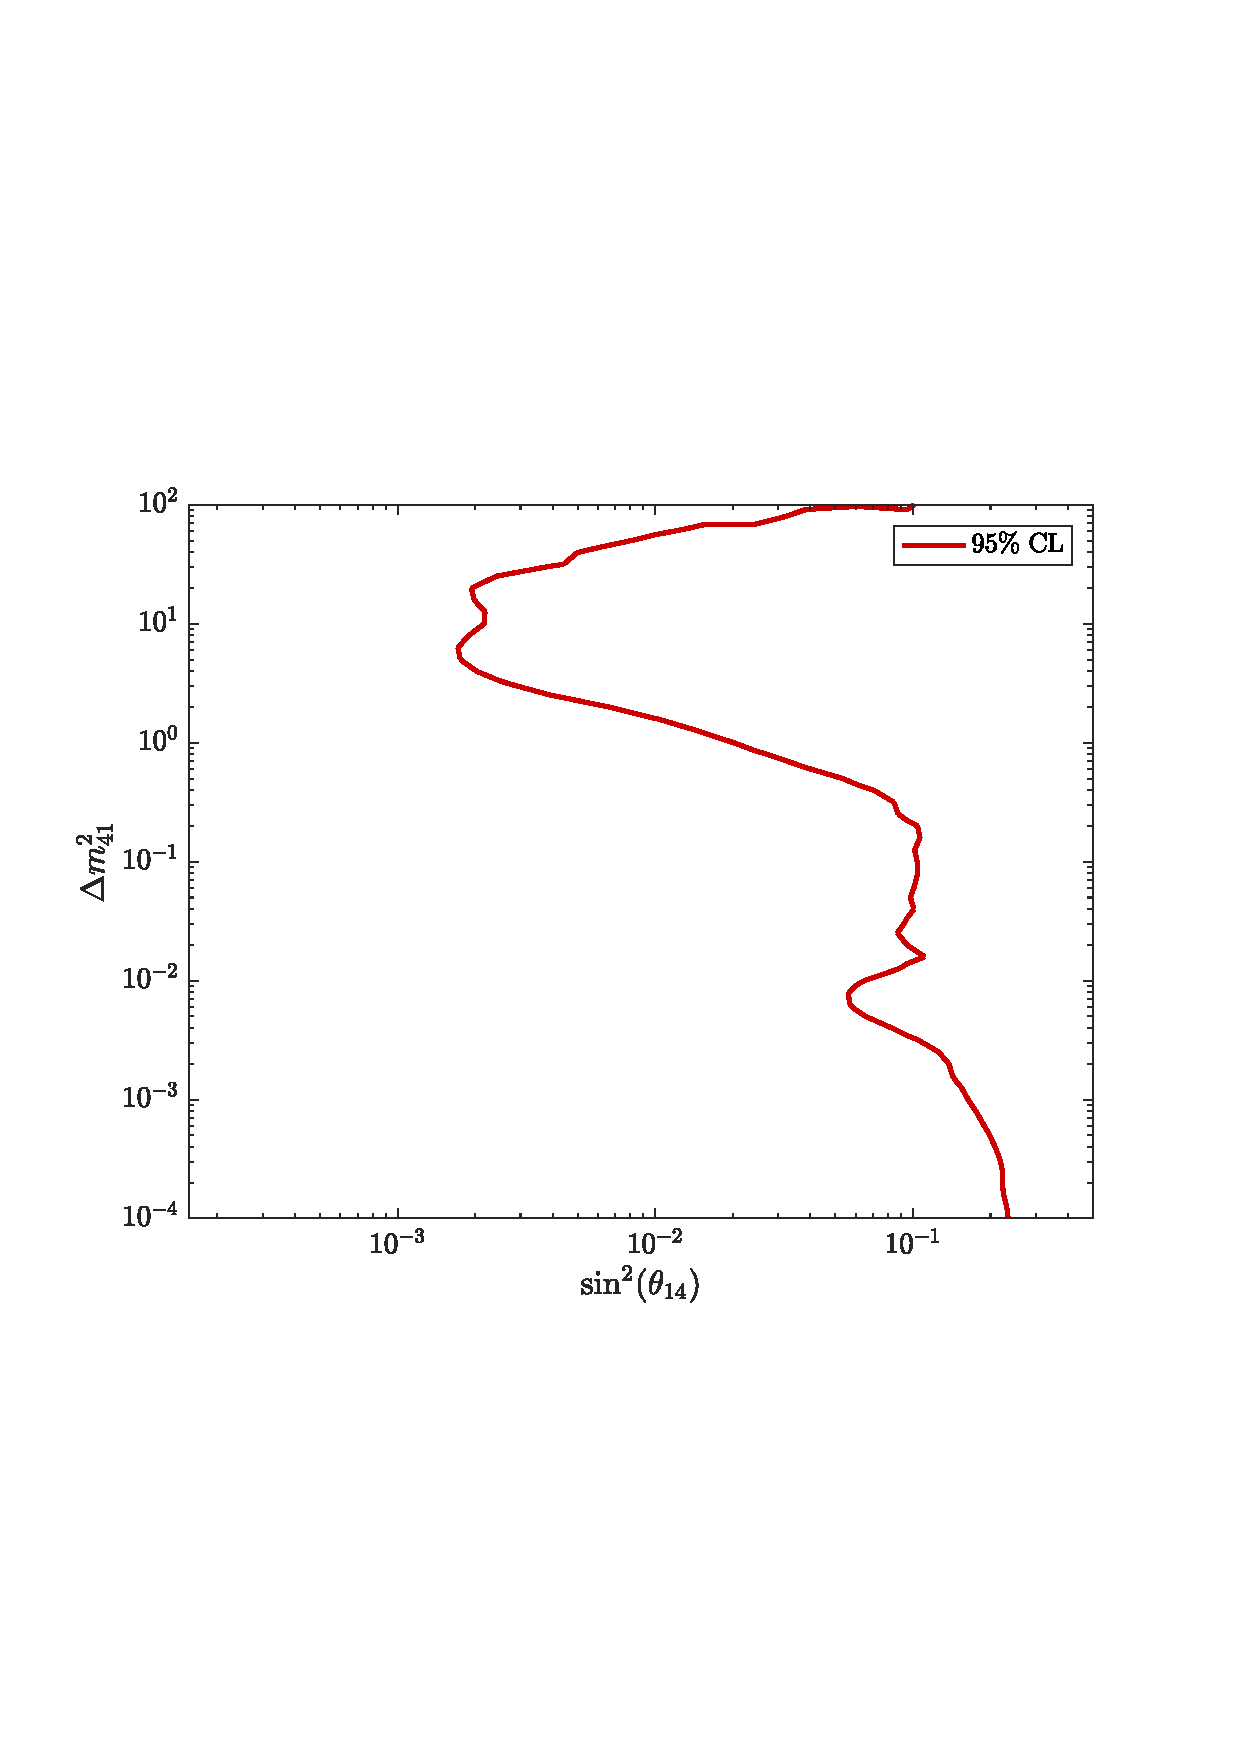
\includegraphics[width=0.45\columnwidth]{th_14_SMR_EOf}}}$
$\vcenter{\hbox{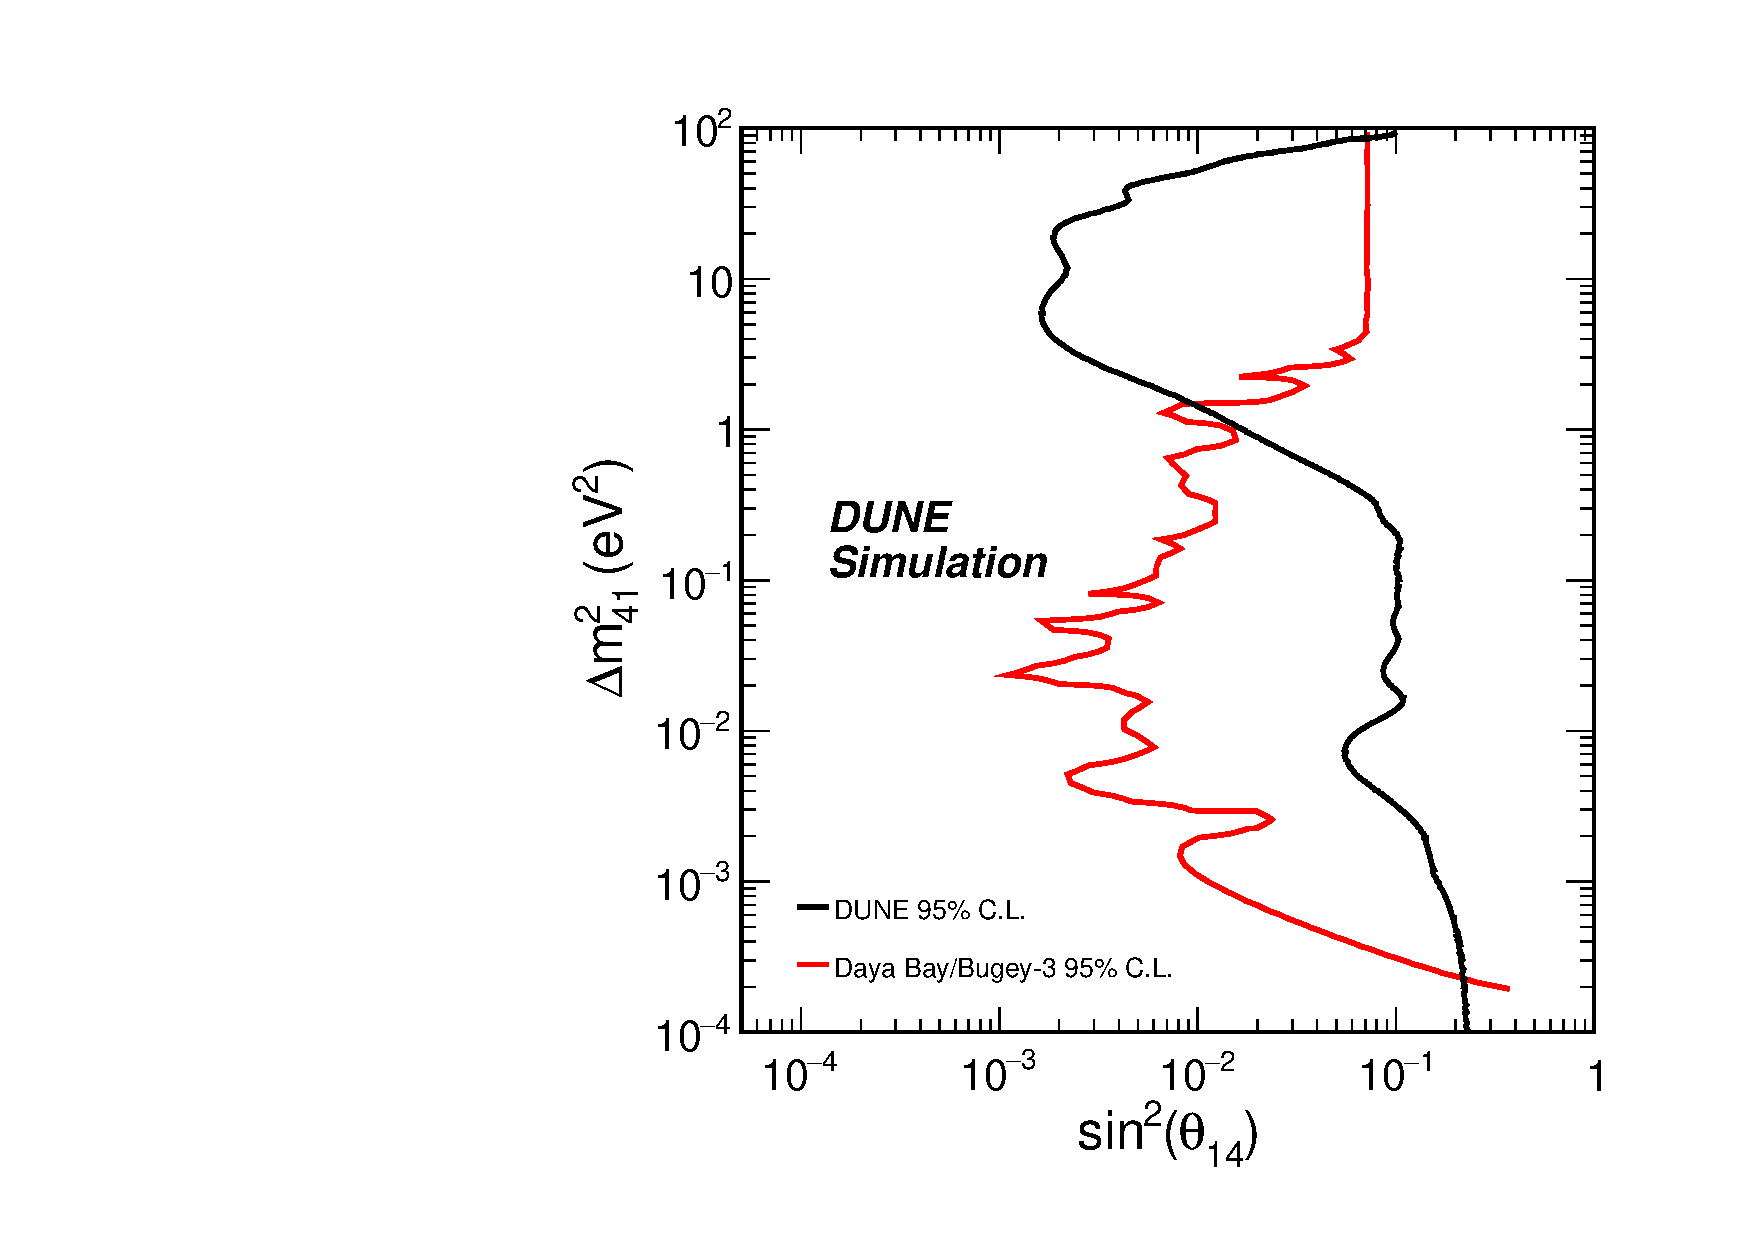
\includegraphics[width=0.45\columnwidth]{MultiPlots_DUNE_th14_prelim}}}$
%\setlength{\abovecaptionskip}{-40pt plus 1pt minus 1pt}
\caption[Sensitivity to $\theta_{14}$ from the $\nu_e$ \dword{cc} samples at near and \dword{fd}s]{The DUNE sensitivity to $\theta_{14}$ from the $\nu_e$ \dword{cc} samples at the near and \dword{fd}s is shown on the left-hand plot. Comparison with the combined reactor result from Daya Bay and Bugey-3 is shown on the right-hand plot. Regions to the right of the contour are excluded.}
\label{th_14}
\end{figure}

For the $\theta_{24}$ mixing angle, we analyze the $\nu_{\mu}$ \dword{cc} disappearance, as well as the \dword{nc} samples, which mainly contribute to the sensitivity. 
\fixme{the samples contribute mainly to the sensitivity (as opposed to contributing to other things)? or they are the main contributors to the sensitivity? anne}
The results are shown in Figure~\ref{th_24}, along with comparisons with present constraints.
\begin{figure}[!htbp]
\centering
%$\vcenter{\hbox{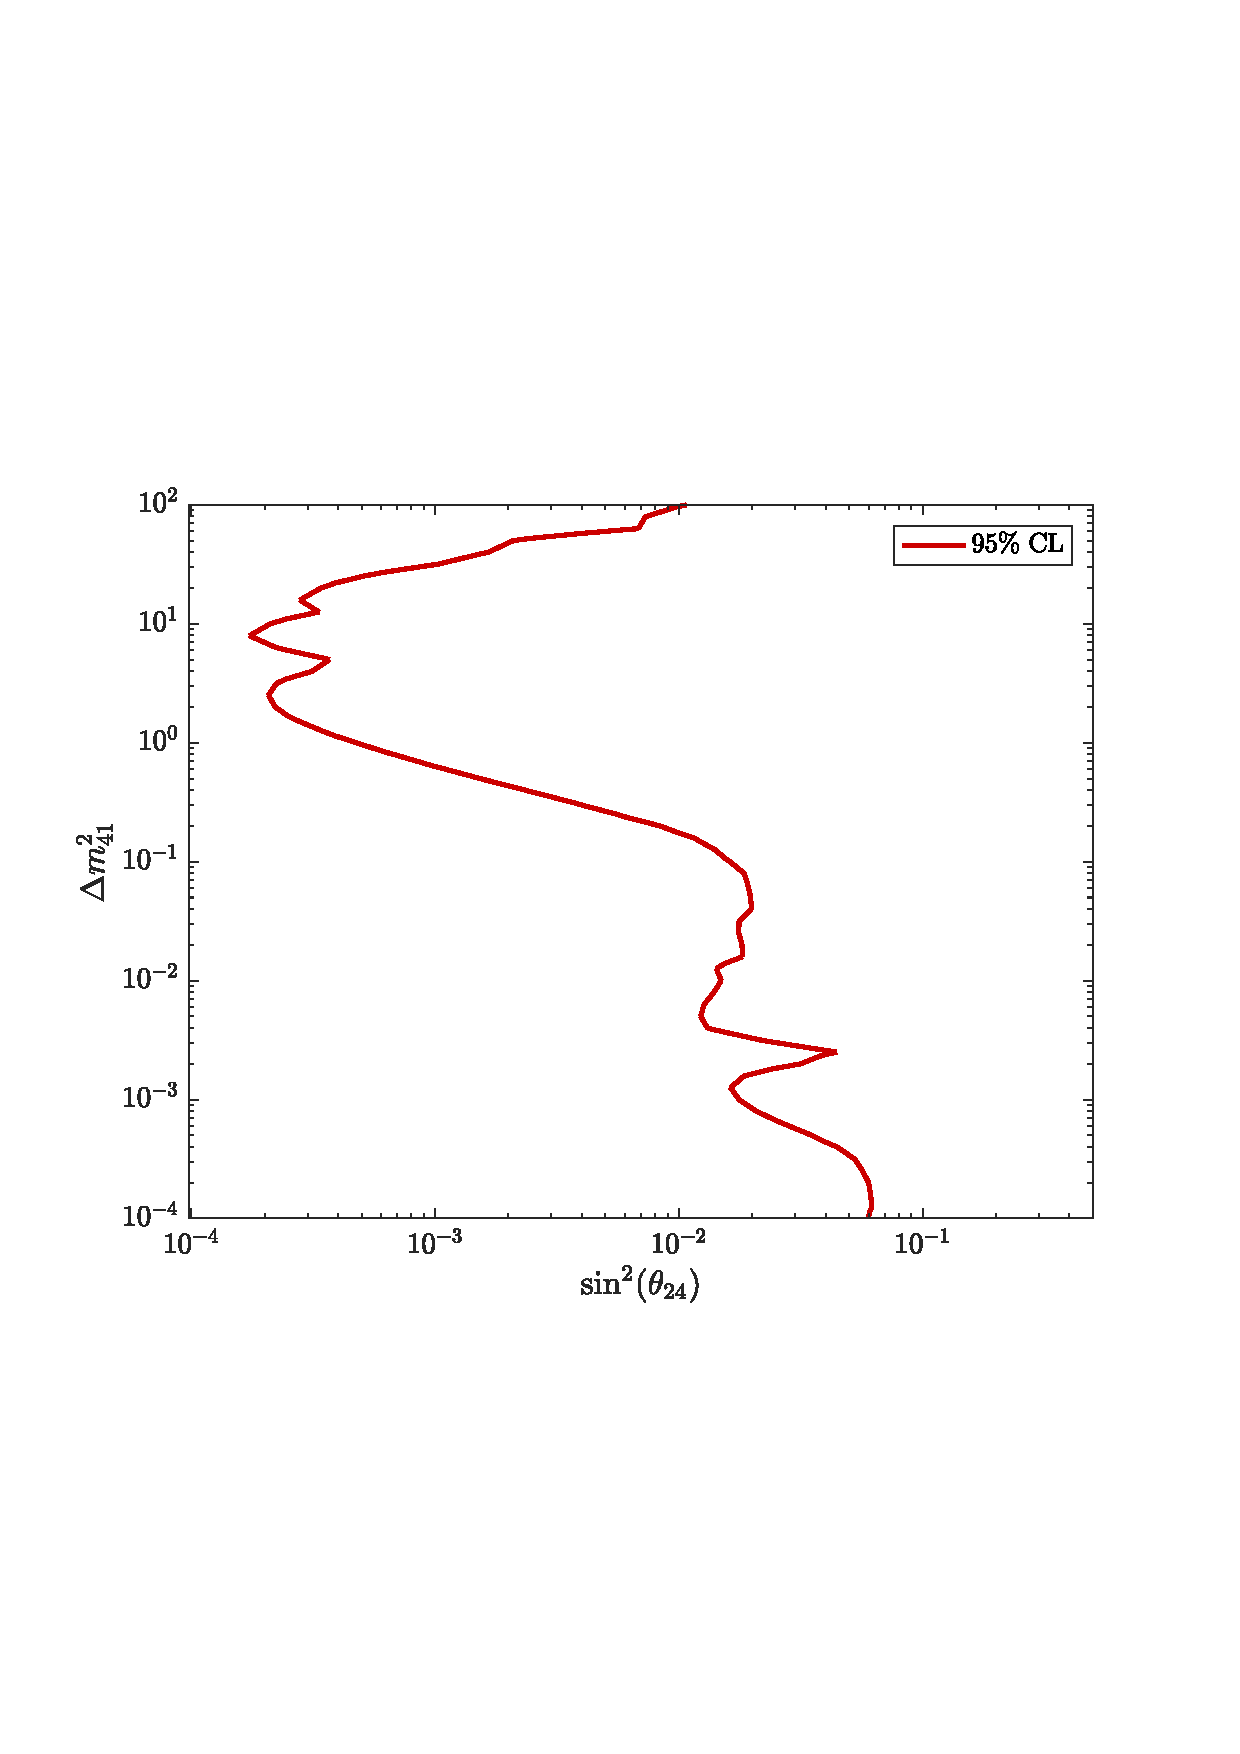
\includegraphics[width=0.45\columnwidth]{th_24_SMR_EOf}}}$
$\vcenter{\hbox{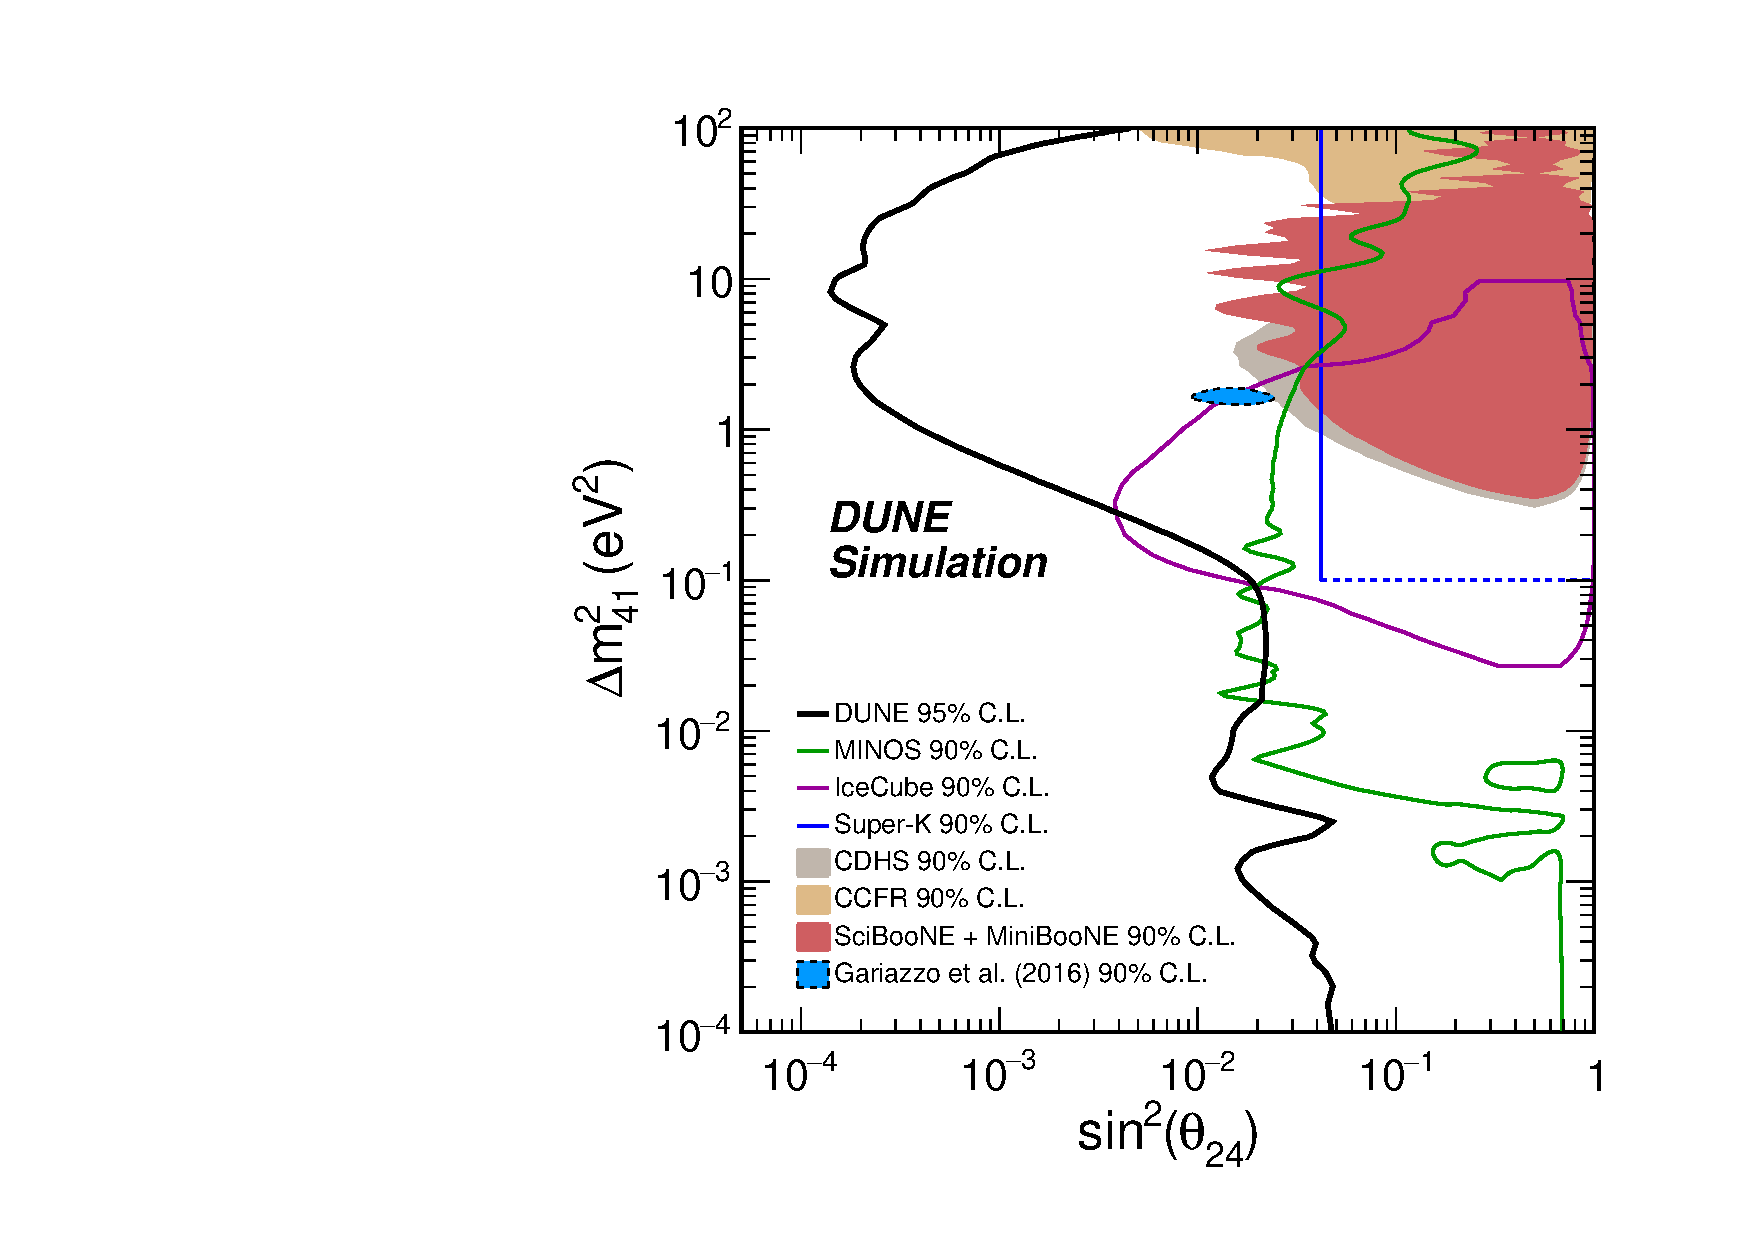
\includegraphics[width=0.45\columnwidth]{MultiPlots_DUNE_MINOS_IceCube_globAppF_prelim.pdf}}}$
%\setlength{\abovecaptionskip}{-40pt plus 1pt minus 1pt}
\caption[Sensitivity to $\theta_{24}$ using the $\nu_\mu$ \dword{cc} and \dword{nc} samples at near and \dword{fd}s]{DUNE sensitivity to $\theta_{24}$ using the $\nu_\mu$ \dword{cc} and \dword{nc} samples at the near and \dword{fd}s is shown on the left-hand plot. A comparison with previous and existing experiments is shown on the right-hand plot. Regions to the right of the contour are excluded.}
\label{th_24}
\end{figure}
    In the case of the $\theta_{34}$ mixing angle, we analyze the \dword{nc} sample, which exclusively contributes to the sensitivity. 
    \fixme{exclusively contributes: it is the only thing that contributes to the sensitivity; contributes exclusively: it contributes to nothing else, but other things may also contribute to the sensitivity. Which?}
    The results are shown in Figure~\ref{th_34}. Further, a comparison with previous experiments sensitive to \numu, \nutau~mixing with large mass-squared splitting is possible by considering an effective mixing angle $\theta_{\mu\tau}$, such that $\sin^2{2\theta_{\mu\tau}}\equiv 4|U_{\tau4}|^2|U_{\mu 4}|^2=\cos^4\theta_{14}\sin^22\theta_{24}\sin^2\theta_{34}$, and assuming conservatively that $\cos^4\theta_{14}=1$, and $\sin^22\theta_{24}=1$. This comparison with previous experiments is also shown in Figure~\ref{th_34}.
\begin{figure}
\centering
%$\vcenter{\hbox{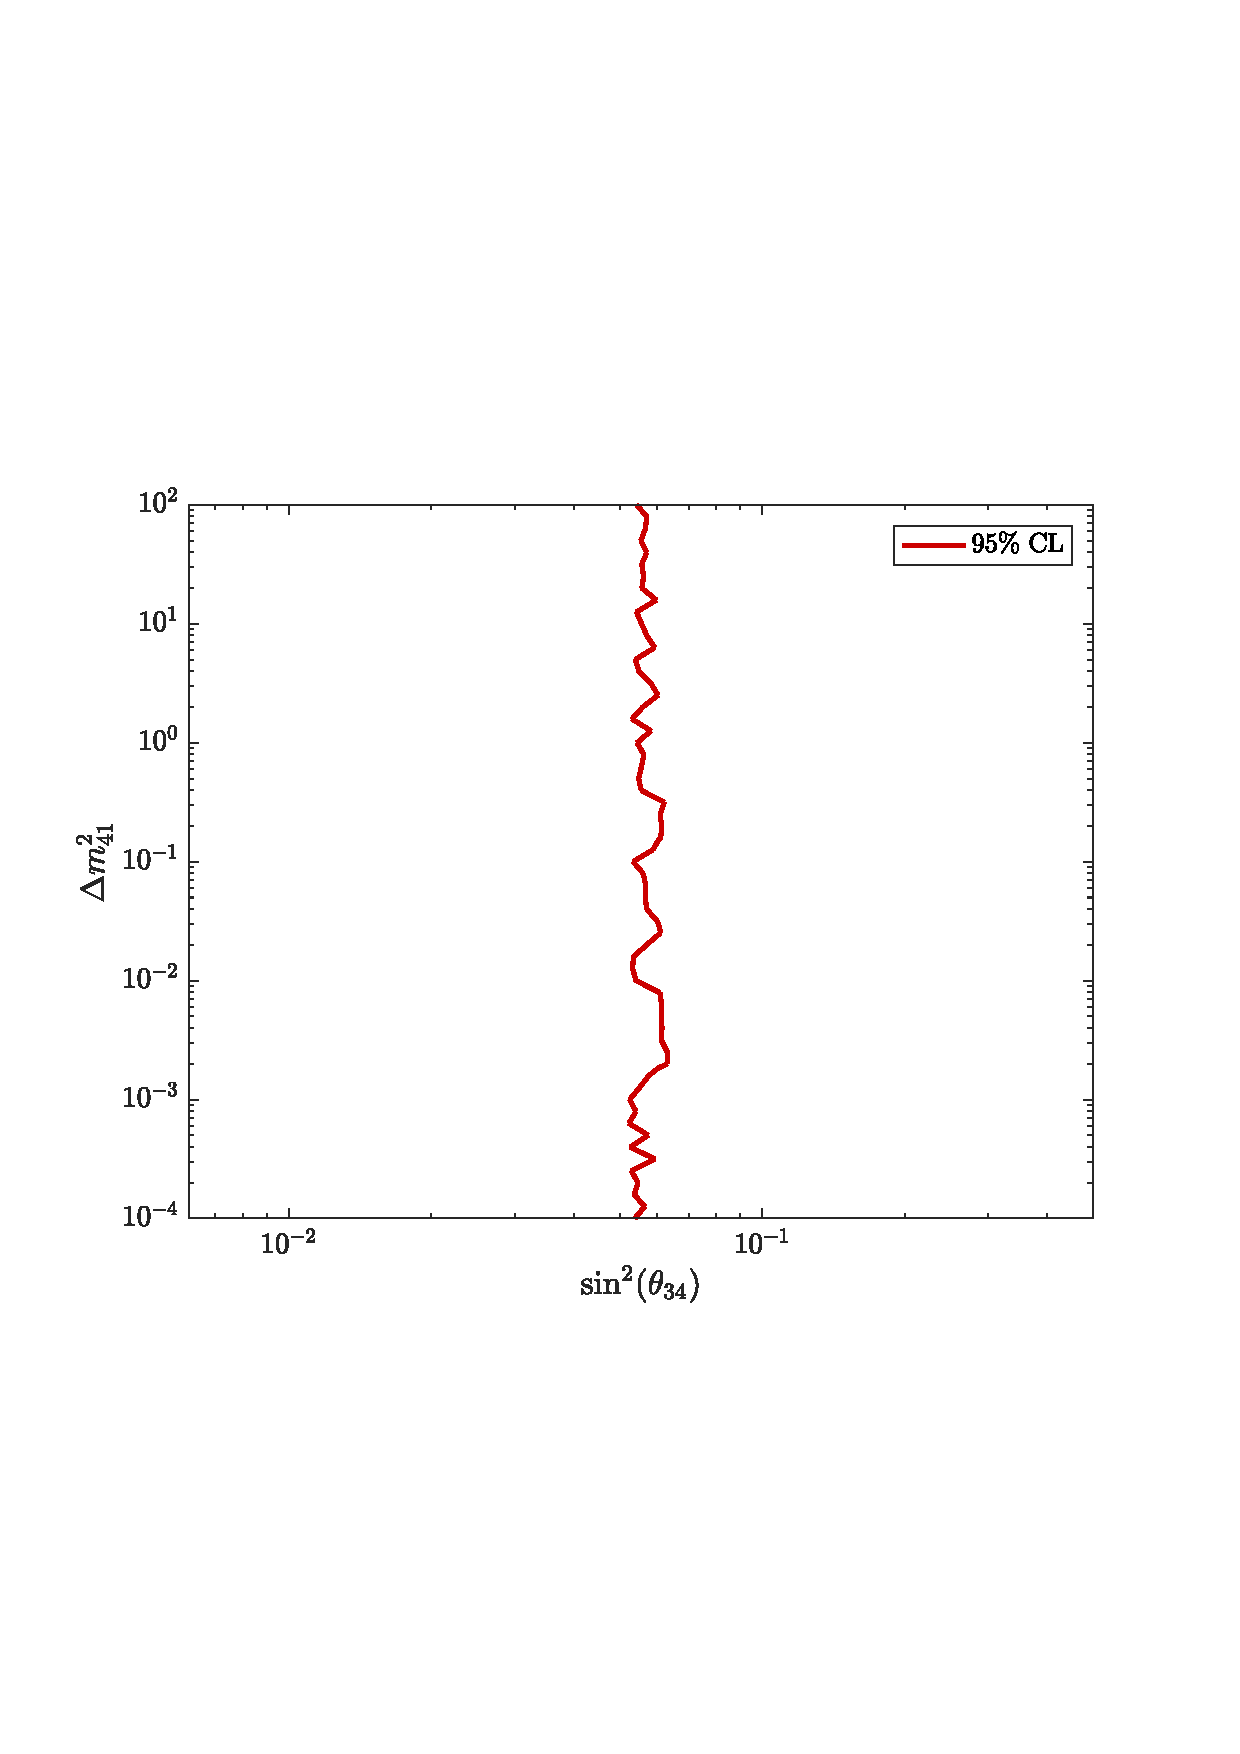
\includegraphics[width=0.45\columnwidth]{th_34_SMR_EOf}}}$
$\vcenter{\hbox{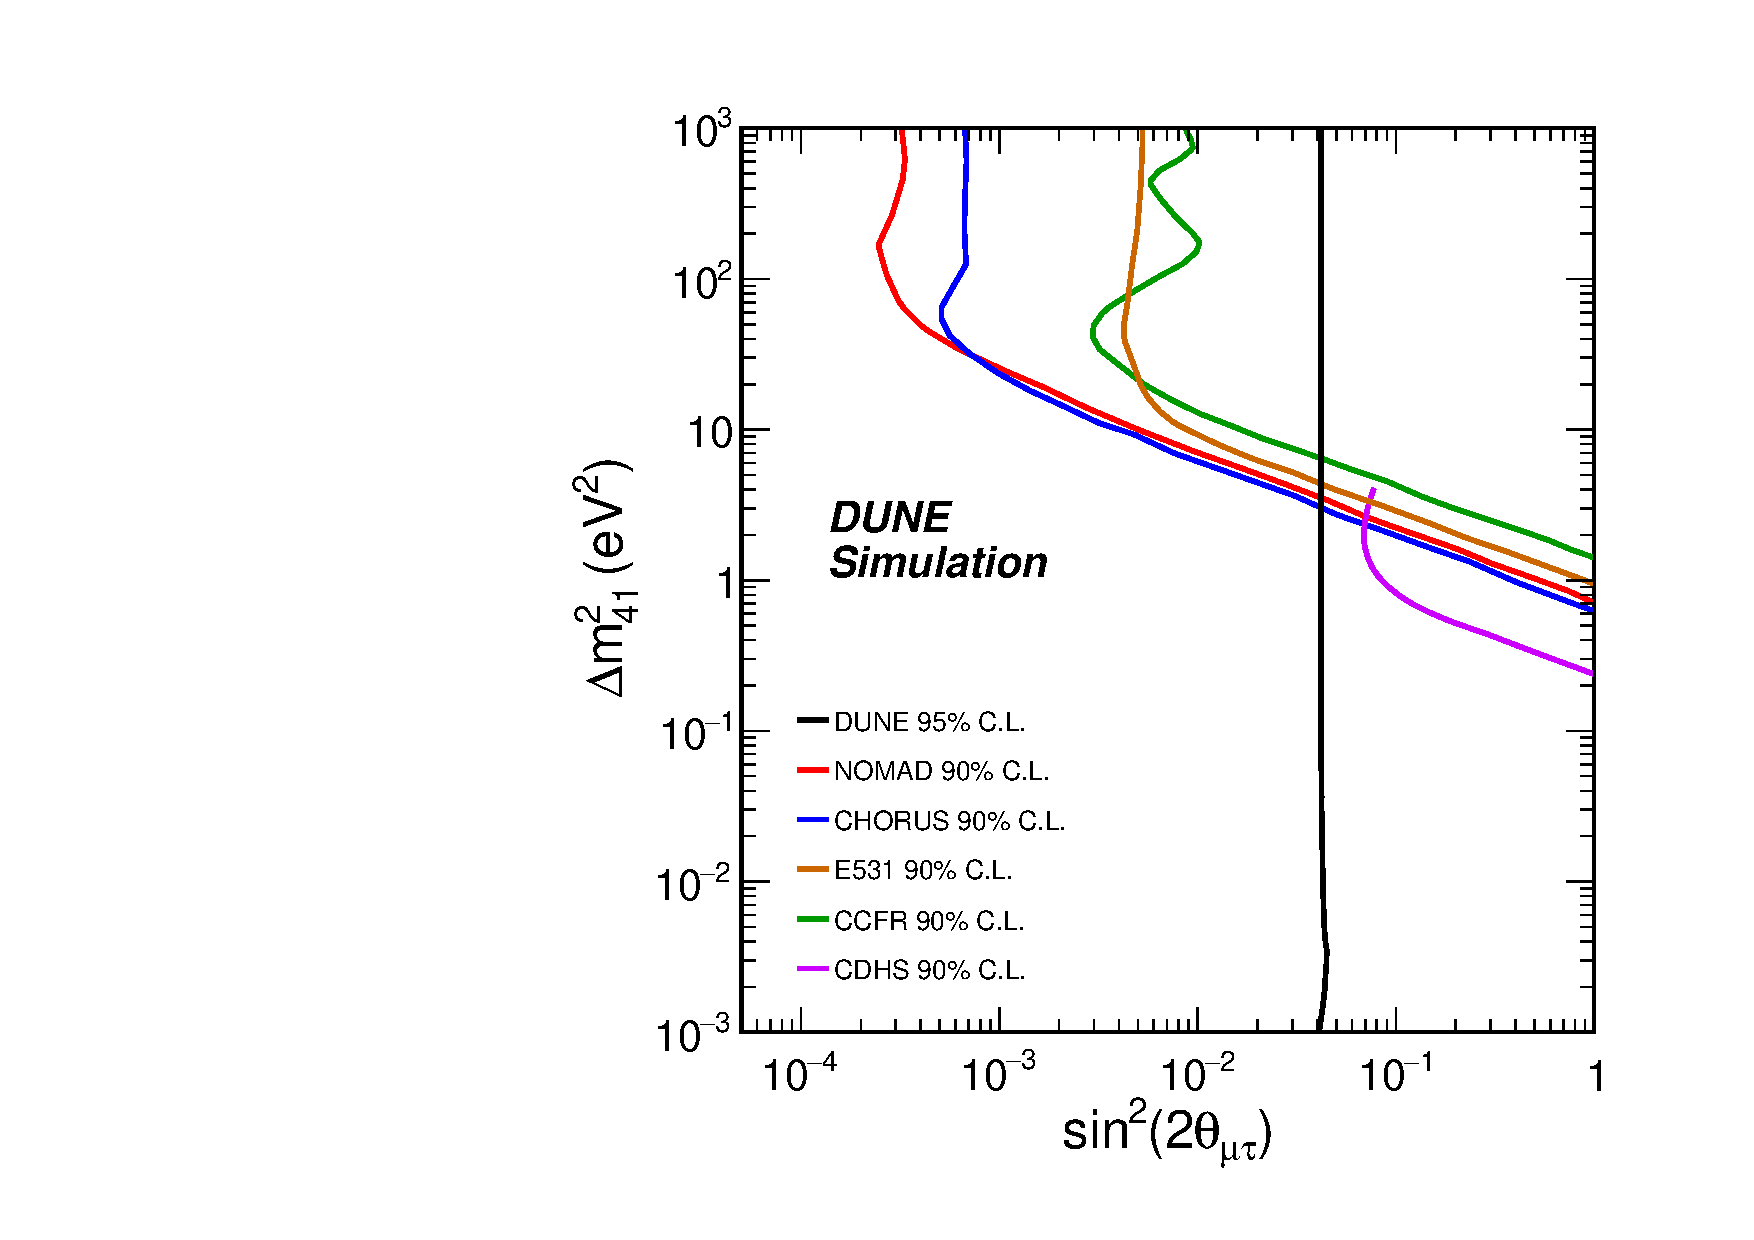
\includegraphics[width=0.45\columnwidth]{MultiPlots_DUNE_th34_prelim}}}$
%\setlength{\abovecaptionskip}{-40pt plus 1pt minus 1pt}
\caption[Sensitivity to $\theta_{34}$ using the \dword{nc} samples at the  \dword{nd} and \dword{fd}]{DUNE sensitivity to $\theta_{34}$ using the \dword{nc} samples at the \dword{nd} and \dword{fd} is shown on the left-hand plot. A comparison with previous and existing experiments is shown on the right-hand plot. Regions to the right of the contour are excluded.}
\label{th_34}
\end{figure}

Another quantitative comparison of our results for $\theta_{24}$ and $\theta_{34}$ with existing constraints can be made for projected upper limits on the sterile mixing angles assuming no evidence for sterile oscillations is found, and picking the value of  $\Delta m^2_{41} = 0.5$~eV$^2$ corresponding to the simpler counting experiment regime. For the $3+1$ model, upper limits of $\theta_{24}$\,$<$\,$2.6^{\circ}$ and $\theta_{34}$\,$<$\,$14.2^{\circ}$ are obtained at the $2\sigma$ or 95\% \dword{cl} from the presented DUNE sensitivities. If expressed in terms of the relevant matrix elements
\begin{align}
|U_{\mu4}|^2 =&\,\,\cos^2\theta_{14}\sin^2\theta_{24} \\
|U_{\tau4}|^2= & \,\,\cos^2\theta_{14}\cos^2\theta_{24}\sin^2\theta_{34},
\label{eq:DisapToApp}
\end{align}
these limits become $|U_{\mu4}|^{2}$\,$<$\,0.002 and $|U_{\tau4}|^{2}$\,$<$\,0.06 at the 95\% \dword{cl}, where we conservatively assume $\cos^2\theta_{14}$\,=\,1 in both cases, and additionally $\cos^2\theta_{24}$\,=\,1 in the second case.
\begin{table}[!ht]
  \centering
  \begin{tabular}{c c c c c }
    \hline\hline
    & $\theta_{24}$ & $\theta_{34}$ & $|U_{\mu4}|^2$ & $|U_{\tau4}|^2$  \\
    \hline
    DUNE  & $2.6^{\circ}$ & $14.2^{\circ}$ & 0.002 & 0.06  \\
    NOvA  & $20.8^{\circ}$ & $31.2^{\circ}$ & 0.126 & 0.268  \\
    %NOvA 2017  & $16.2^{\circ}$ & $29.8^{\circ}$ & 0.078 & 0.220 \\
    MINOS & $7.3^{\circ}$ & $26.6^{\circ}$ & 0.016 & 0.20  \\
    \superk & $11.7^{\circ}$ & $25.1^{\circ}$ & 0.041 & 0.18  \\
    IceCube & $4.1^{\circ}$ & \-- & 0.005 & \--   \\
    IceCube-DeepCore & $19.4^{\circ}$ & $22.8^{\circ}$ & 0.11 & 0.15  \\
    \hline\hline
  \end{tabular}%
    \caption[Projected 95\% \dword{cl} upper limits on sterile mixing angles and matrix elements]{The projected DUNE 95\% \dword{cl} upper limits on sterile mixing angles and matrix elements compared to the equivalent 90\% \dword{cl} upper limits from \nova~\cite{ref:novasterile}, MINOS~\cite{ref:minossterile}, \superk~\cite{ref:superksterile}, IceCube~\cite{ref:IceCube}, and IceCube-DeepCore~\cite{ref:DeepCore}. The limits are shown for $\Delta m^2_{41} = 0.5$~eV$^2$ for all experiments, except for IceCube-DeepCore, where the results are reported for $\Delta m^2_{41} = 1.0$~eV$^2$.}
  \label{tab:limits}
\end{table}  
  
  
Finally, sensitivity to the $\theta_{\mu e}$ effective mixing angle, defined above as $\sin^2{2\theta_{\mu e}}\equiv 4|U_{e4}|^2|U_{\mu 4}|^2=\sin^22\theta_{14}\sin^2\theta_{24}$, is shown in Figure~\ref{th_me}, which also displays a comparison with the allowed regions from \dword{lsnd} and MiniBooNE, as well as with present constraints and projected constraints from the \fnal \dword{sbn} program.
\begin{figure}[!htbp]
\centering
%$\vcenter{\hbox{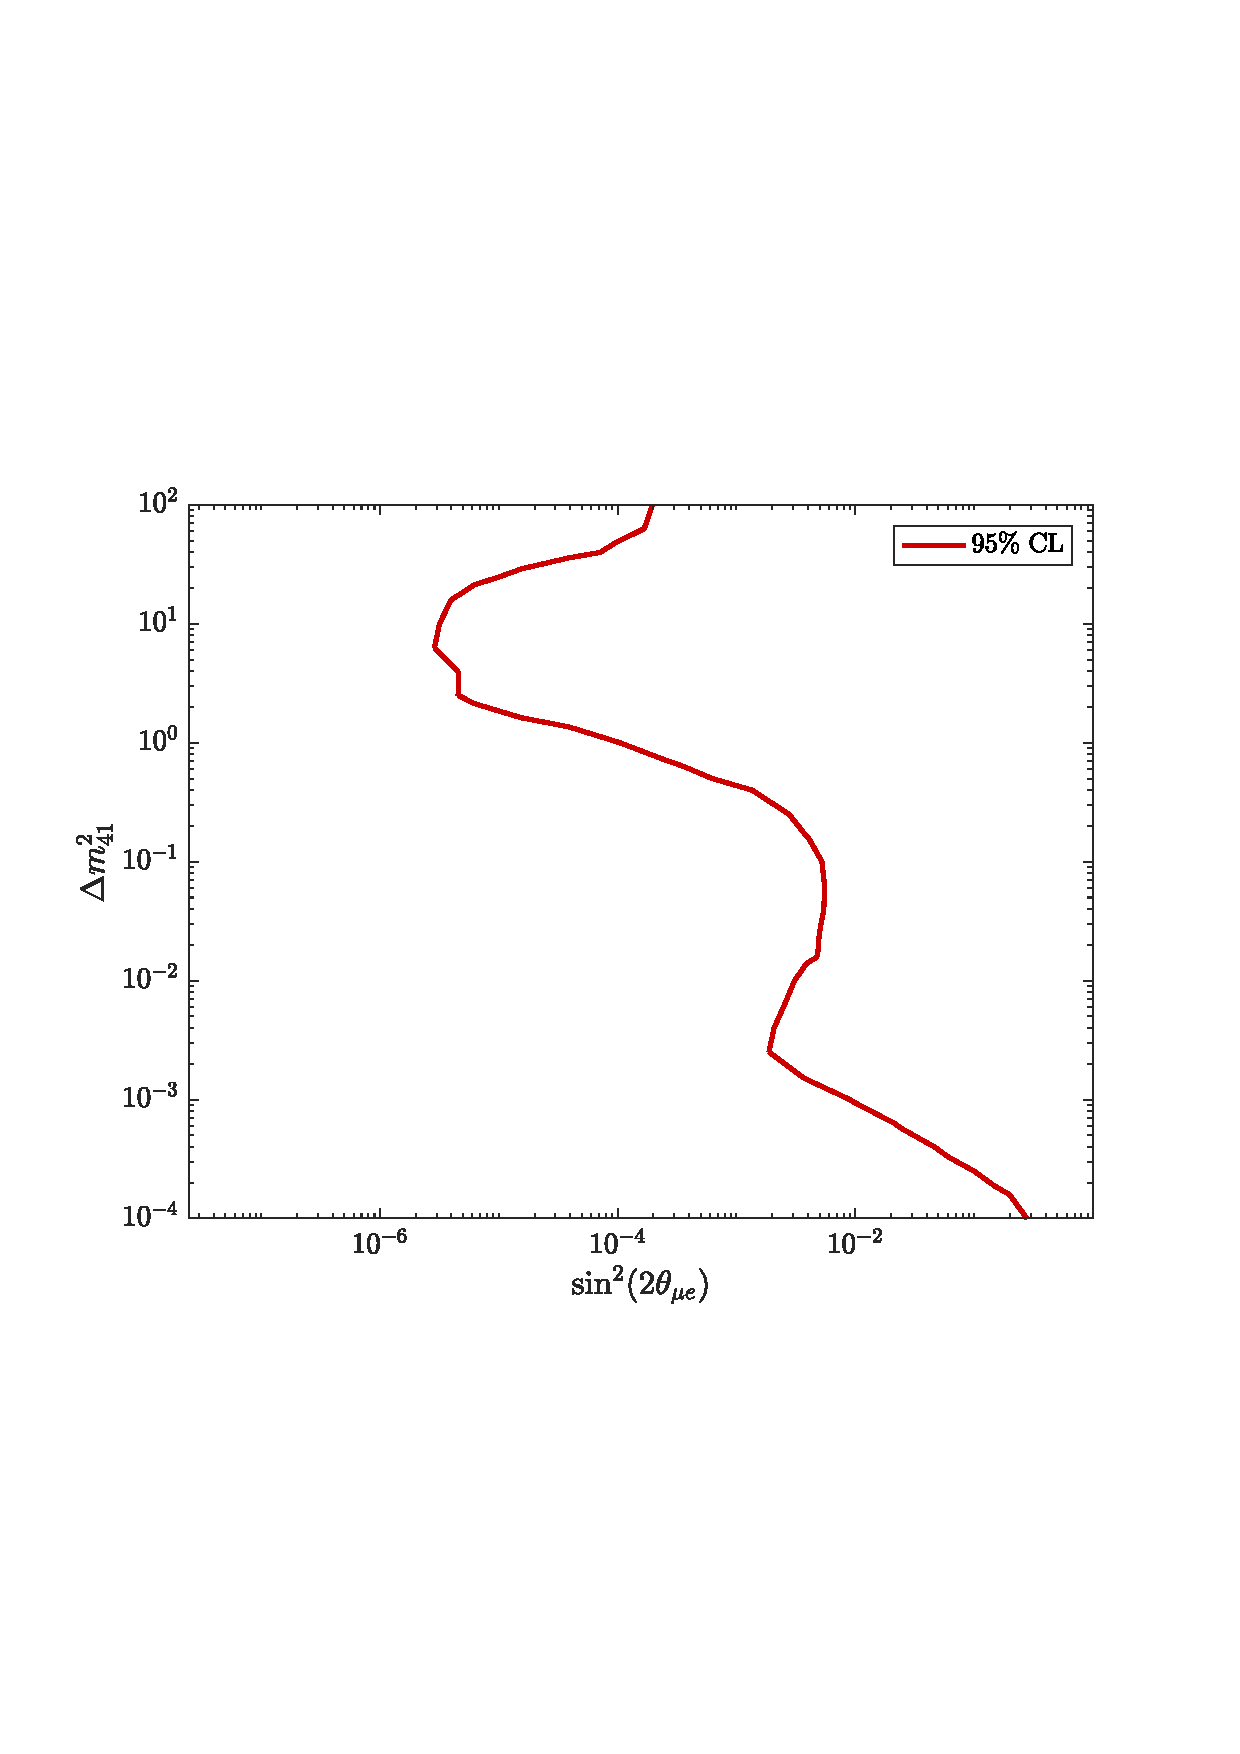
\includegraphics[width=0.45\columnwidth]{th_me_SMR_EOf}}}$
$\vcenter{\hbox{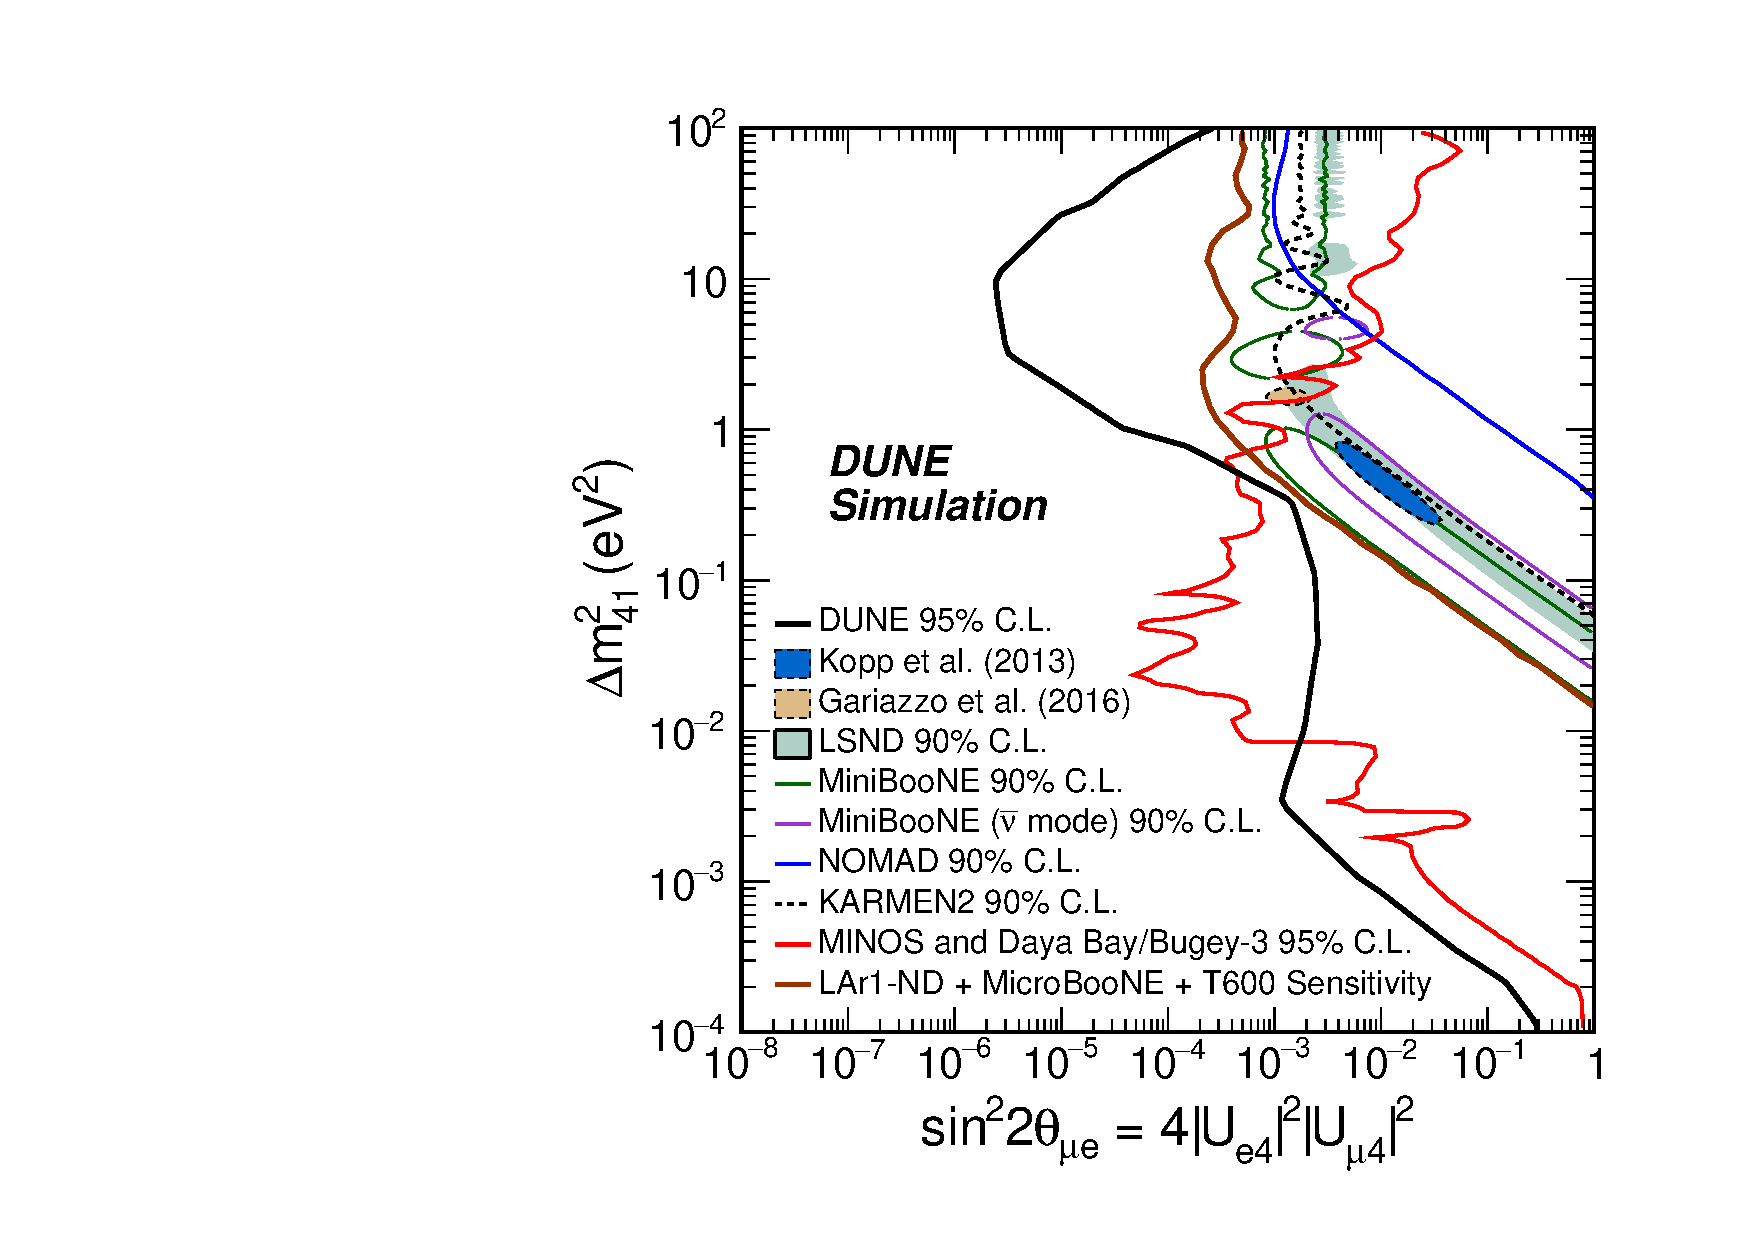
\includegraphics[width=0.45\columnwidth]{ComboLimit95_dune_sbn.pdf}}}$
%\setlength{\abovecaptionskip}{-40pt plus 1pt minus 1pt}
\caption[Sensitivity to $\theta_{\mu e}$ from the appearance and disappearance samples]{DUNE sensitivity to $\theta_{\mu e}$ from the appearance and disappearance samples at the Near and \dword{fd}s is shown on the left-hand plot. A comparison with previous existing experiments and the sensitivity from the future \dword{sbn} program is shown on the right-hand plot. Regions to the right of the contour are excluded.}
\label{th_me}
\end{figure}

To illustrate that DUNE would not be limited to constraining regions of parameter space describing active-sterile neutrino mixing, we have produced a discovery potential plot, for a scenario with one sterile neutrino governed by the \dword{lsnd} best-fit parameters $\left(\Delta m_{14}^2= 1.2\;\text{eV}^2;\,\,\sin^2{2\theta_{\mu e}}=0.003\right)$~\cite{LSNDSterile}. A small $2\sigma$ allowed region, shown in Figure~\ref{Dis_plot_me}, is obtained, which can be compared with the \dword{lsnd} allowed region in Figure~\ref{th_me}. 
\begin{figure}[!h]
\centering
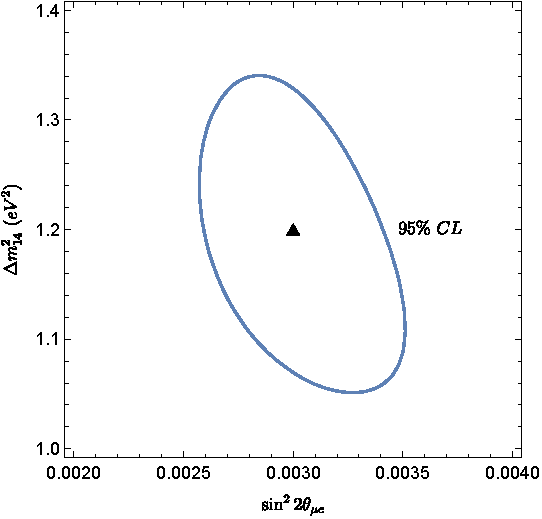
\includegraphics[scale=0.8]{dpme}
\caption[Discovery plot assuming $\theta_{\mu e}$ and $\Delta m_{41}^2$ are at the \dword{lsnd} anomaly best-fit point]{Discovery plot assuming $\theta_{\mu e}$ and $\Delta m_{41}^2$ are at the \dword{lsnd} anomaly best-fit point~\cite{LSNDSterile}.}
\label{Dis_plot_me}
\end{figure}

The physics reach plots shown above illustrate the excellent potential of DUNE to discover or constrain mixing with sterile neutrinos. Notably, in the case of sterile-mediated \numu~to \nue~transistions, DUNE can place very competitive constraints on its own, without requiring a combination with reactor experiments. 

%\subsection{Discussion of potential enhancements from hardware improvements}
These studies show compelling motivation for DUNE to deploy a highly-capable \dword{nd}  given its high potential for discovery or constraining of new physics, including mixing with sterile neutrino species.


%%% NEUTRINO TRIDENTS %%%%%%%%%%%%%%%%%%%%%%%%
\section{Search for Neutrino Tridents at the Near Detector}


Neutrino trident production is a weak process in which a neutrino, scattering off the Coulomb field of a heavy nucleus, generates a pair of charged leptons ~\cite{Czyz:1964zz,Lovseth:1971vv,Fujikawa:1971nx,Koike:1971tu,Koike:1971vg,Brown:1973ih,Belusevic:1987cw}. Measurements of muonic neutrino tridents ($\nu_\mu \to \nu_\mu \mu^+\mu^-$) were carried out at the CHARM-II~\cite{Geiregat:1990gz}, CCFR~\cite{Mishra:1991bv} and NuTeV~\cite{Adams:1999mn} experiments:


\[
\frac{\sigma(\nu_\mu \to \nu_\mu \mu^+\mu^-)_\text{exp}}{\sigma(\nu_\mu \to \nu_\mu \mu^+\mu^-)_\text{SM}} = 
\begin{cases}
1.58 \pm 0.64         & \text{(CHARM-II)} \\ 
0.82 \pm 0.28         & \text{(CCFR)} \\
0.72 ^{+1.73}_{-0.72} & \text{(NuTeV)} 
\end{cases}
\]
%%%%%%%%%%
The high-intensity muon-neutrino beam at the DUNE \dword{nd}  will lead to a sizable production rate of trident events (see Table~\ref{tab:trident_rates}), offering excellent prospects to improve the above measurements. A deviation from the event rate predicted by the \dword{sm} could be an indication of new interactions mediated by the corresponding new gauge bosons~\cite{Altmannshofer:2014pba}. 

%%%%%%%%%%%%%%%%%%%%%%%%%%%%%%
\begin{table}[!b]
\begin{center}
\begin{tabular}{lcccc}
\toprule
& \multicolumn{2}{c}{Reference beam, 80~GeV} & \multicolumn{2}{c}{Optimized beam, 120~GeV} \\
& coherent & incoherent & coherent & incoherent \\
\midrule
$\nu_\mu \to \nu_\mu \mu^+\mu^-$ & $2.05 \pm 0.12$ & $0.87 \pm 0.27$ & $1.17 \pm 0.07$ & $0.49 \pm 0.15$ \\
$\nu_\mu \to \nu_\mu e^+e^-$ & $4.92 \pm 0.29$ & $0.32 \pm 0.10$ & $2.84 \pm 0.17$ & $0.18 \pm 0.06$\\
$\nu_\mu \to \nu_e e^+\mu^-$ & $17.4 \pm 1.0$ & $2.2 \pm 0.7$ & $9.8 \pm 0.6$ & $1.2 \pm 0.4$ \\
$\nu_\mu \to \nu_e \mu^+e^-$ & $0$ & $0$ & $0$ & $0$ \\
\midrule
$\bar\nu_\mu \to \bar\nu_\mu \mu^+\mu^-$ & $1.54 \pm 0.09$ & $0.67 \pm 0.21$ & $0.72 \pm 0.04$ & $0.32 \pm 0.10$ \\
$\bar\nu_\mu \to \bar\nu_\mu e^+e^-$ & $4.03 \pm 0.24$ & $0.26 \pm 0.08$ & $2.21 \pm 0.13$ & $0.13 \pm 0.04$ \\
$\bar\nu_\mu \to \bar\nu_e e^+\mu^-$ & $0$ & $0$ & $0$ & $0$ \\
$\bar\nu_\mu \to \bar\nu_e \mu^+e^-$ & $13.8 \pm 0.8$ & $1.7 \pm 0.5$ & $7.0 \pm 0.4$ & $0.9 \pm 0.3$ \\
\bottomrule
\end{tabular}
\end{center}
\caption[Expected number of \dword{sm} $\nu_\mu$ and $\bar\nu_\mu$-induced trident events at \dword{nd} per ton of argon and year of operation]{Expected number of \dword{sm}  $\nu_\mu$ and $\bar\nu_\mu$-induced trident events at the DUNE \dword{nd}  per metric on of argon and year of operation, and for two neutrino beam configurations, the 80~GeV reference beam from the DUNE \dword{cdr}~\cite{cdr-vol-2} and the engineered optimized 120~GeV beam from~\cite{fields_doc_2901}. We assume $1.47 \times 10^{21}$~POT per year for the 80~GeV beam~\cite{cdr-vol-2} and  $1.1 \times 10^{21}$~POT per year for the 120~GeV beam~\cite{fields_doc_2901}.}
\label{tab:trident_rates}
\end{table}
%%%%%%%%%%%%%%%%%%%%%%%%%%%%%%

The main challenge in obtaining a precise measurement of the muonic trident cross section will be the copious backgrounds, mainly consisting of \dword{cc} single-pion production events, $\nu_\mu N \to \mu \pi N^\prime$, as muon and pion tracks can be easily confused in LArTPC detectors. The discrimination power of the DUNE \dword{nd} LArTPC was evaluated using large simulation datasets of signal and background. Each simulation event represents a different neutrino-argon interaction in the active volume of the detector. Signal events were generated using a standalone code \cite{} that simulates trident production of muons and electrons through the scattering of $\nu_{mu}$ and $\nu_e$ on argon or iron nuclei. The generator considers both the coherent scattering on the full nucleus (the dominant contribution) and the incoherent scattering on individual nucleons. Background events, consisting of several \dword{sm} neutrino interactions, were generated using \dword{genie}. Roughly $30\%$ of the generated events have a charged pion in the final state, leading to two charged tracks with muon-like energy deposition pattern ($\mathrm{d}E/\mathrm{d}x$), as in our trident signal. All final-state particles produced in the interactions were propagated through the detector geometry using the Geant4-based \cite{Agostinelli:2002hh,Allison:2006ve,Allison:2016lfl} simulation of the DUNE \dword{nd}. Charge collection and readout were not simulated, and possible inefficiencies due to mis-reconstruction effects or event pile-up were disregarded for simplicity.

%%%%%%%%%%%%%%%%%%%%%%%%%%%%%%
\begin{figure}[!tb]
\centering
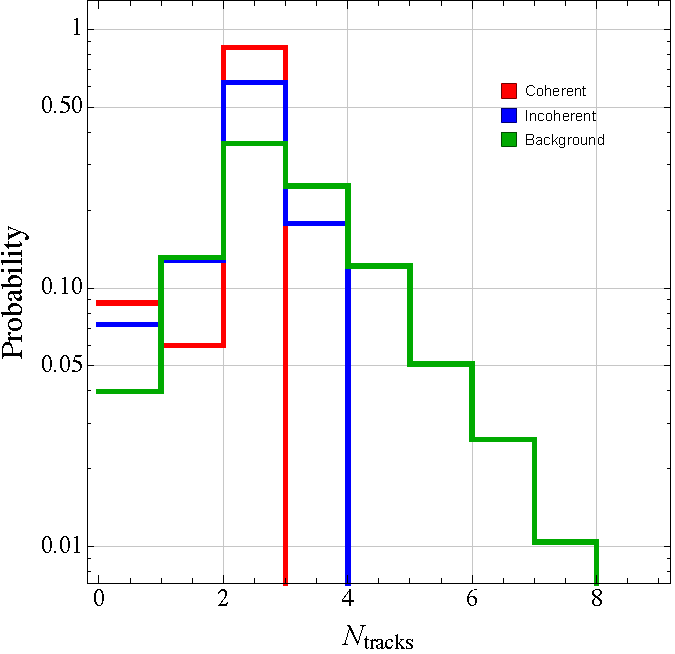
\includegraphics[height=5cm]{NTracksHistogram.pdf}
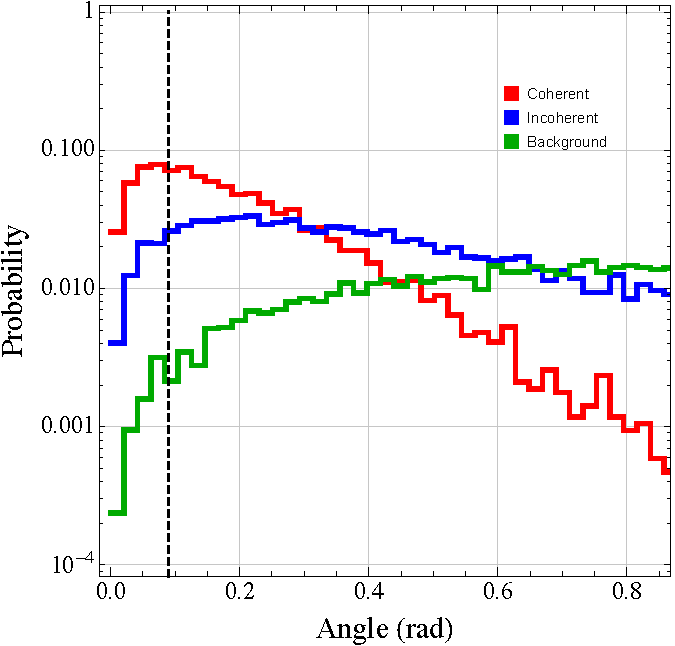
\includegraphics[height=5cm]{AngleHistogram.pdf} \\[0.75\baselineskip]
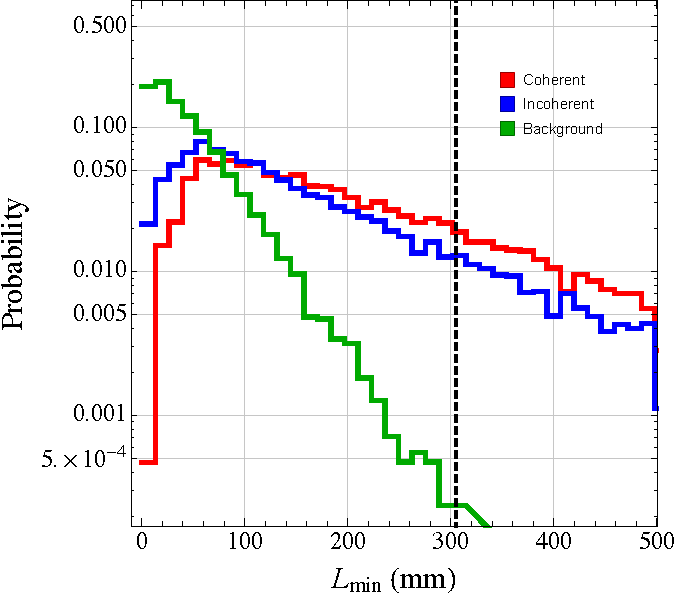
\includegraphics[height=5cm]{LengthHistogram.pdf}
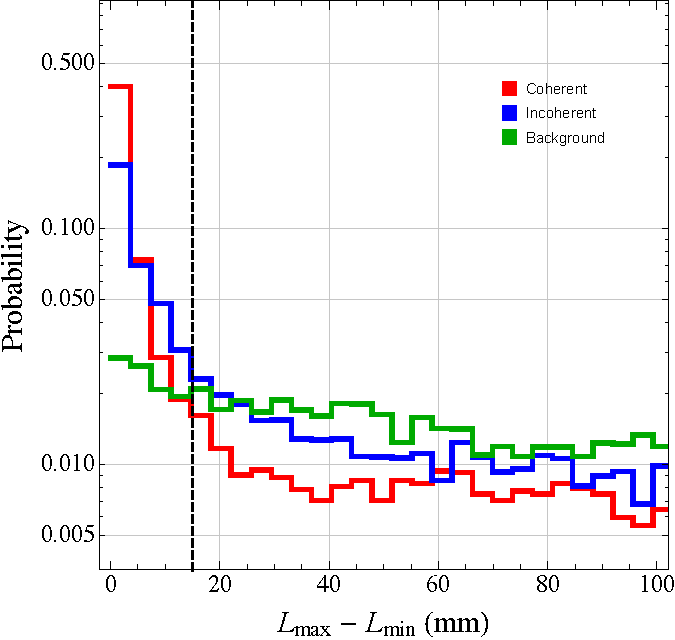
\includegraphics[height=5cm]{DeltaLHistogram.pdf}
\caption[Kinematic distributions of signal and background considered for the selection of muonic trident interactions in the \dword{nd} LArTPC]{Event kinematic distributions of signal and background considered for the selection of muonic trident interactions in the \dword{nd} LArTPC: number of tracks (top left), angle between the two main tracks (top right), length of the shortest track (bottom left), and the difference in length between the two main tracks (bottom right). The dashed, black vertical lines indicate the optimal cut values used in the analysis.} \label{fig:trident_kinematics}
\end{figure}
%%%%%%%%%%%%%%%%%%%%%%%%%%%%%%

Figure~\ref{fig:trident_kinematics} shows the distribution (area normalized) for signal and background of the different kinematic variables used in our analysis for the discrimination between signal and background. As expected, background events tend to contain a higher number of tracks than the signal. The other distributions also show a clear discriminating power: the angle between the two tracks is typically much smaller in the signal than in the background. Moreover, the signal tracks (two muons) tend to be longer than tracks in the background (mainly one muon plus one pion).

%%%%%%%%%%%%%%%%%%%%%%%%%%%%%%%%%%%%%%%%
\section{Sensitivity to New Physics} %Anne changed from sub to section; can't have just one 

The sensitivity of neutrino tridents to heavy new physics (i.e., heavy compared to the momentum transfer in the process) can be parametrized in a model-independent way using a modification of the effective four-fermion interaction Hamiltonian. Focusing on the case of muon-neutrinos interacting with muons, the vector and axial-vector couplings can be written as
%%%%%%%%%%
\begin{equation}
g_{\mu\mu\mu\mu}^V = 1 + 4 \sin^2\theta_W + \Delta g_{\mu\mu\mu\mu}^V \quad \mathrm{and} \quad g_{\mu\mu\mu\mu}^A = -1 + \Delta g_{\mu\mu\mu\mu}^A ~,
\end{equation}
%%%%%%%%%%
where $\Delta g_{\mu\mu\mu\mu}^V$ and $\Delta g_{\mu\mu\mu\mu}^A$ parameterize possible new physics contributions. Couplings involving other combinations of lepton flavors can be modified analogously. Note, however, that for interactions that involve electrons, very strong constraints can be derived from LEP bounds on electron contact interactions~\cite{Schael:2013ita}. The modified interactions of the muon-neutrinos with muons alter the cross section of the $\nu_\mu N \to \nu_\mu \mu^+\mu^- N$ trident process. In Figure~\ref{fig:trident_gVgA} we show the regions in the $\Delta g^V_{\mu\mu\mu\mu}$ vs.\ $\Delta g^A_{\mu\mu\mu\mu}$ plane that are excluded by the existing CCFR measurement $\sigma_\text{CCFR} / \sigma_\text{CCFR}^\text{SM} = 0.82 \pm 0.28$~\cite{Mishra:1991bv} at the 95\% \dword{cl} in gray. A measurement of the $\nu_\mu N \to \nu_\mu \mu^+\mu^- N$ cross section with $25\%$ uncertainty at the DUNE \dword{nd}  could cover the blue hashed regions. We see that the DUNE measurement could extend the coverage of new physics parameter space substantially.

%%%%%%%%%%%%%%%%%%%%%%%%%%%%%%%%%%%%%%%%%%%%%%%%%%%%%%%%%%%%%%%
\begin{figure}[tb!]
\centering
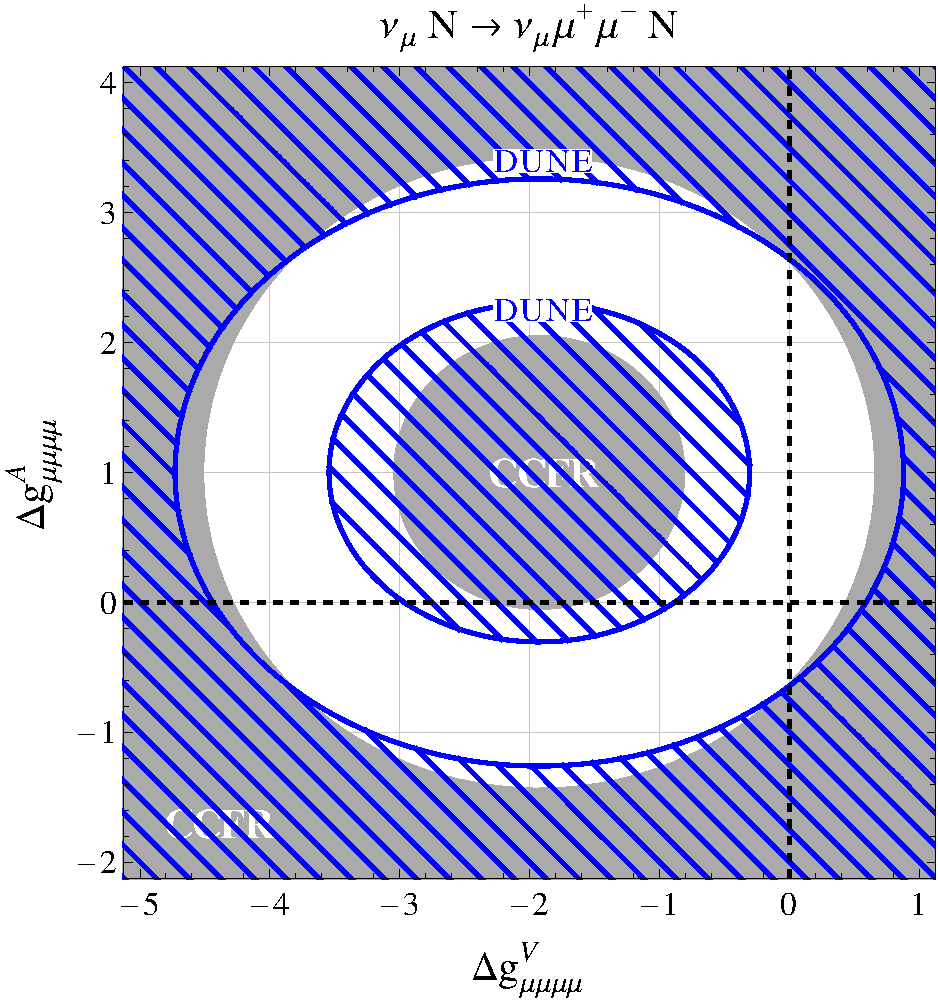
\includegraphics[width=0.4\textwidth]{model_independent.pdf}
\caption[Projected sensitivity of $\nu_\mu N \to \nu_\mu \mu^+\mu^- N$ cross section at the \dword{nd} to modifications of the vector and axial-vector couplings of \numu{}s to muons]{Projected sensitivity (95\% \dword{cl}) of a measurement of the $\nu_\mu N \to \nu_\mu \mu^+\mu^- N$ cross section at the DUNE \dword{nd}  to modifications of the vector and axial-vector couplings of muon-neutrinos to muons (blue hashed regions). The gray regions are excluded at 95\% \dword{cl} by existing measurements of the cross section by the CCFR collaboration. The intersection of the dashed lines indicates the \dword{sm} point.}
\label{fig:trident_gVgA}
\end{figure}
%%%%%%%%%%%%%%%%%%%%%%%%%%%%%%%%%%%%%%%%%%%%%%%%%%%%%%%%%%%%%%%

A class of models that modify the trident cross section are those that contain an additional neutral gauge boson, $Z'$, that couples to neutrinos and charged leptons. A consistent way of introducing such a $Z'$ is to gauge an anomaly-free global symmetry of the \dword{sm}. Of particular interest is the $Z'$ that is based on gauging the difference of muon-number and tau-number, $L_\mu - L_\tau$~\cite{He:1990pn,He:1991qd}. Such a $Z'$ is relatively weakly constrained and can for example address the longstanding discrepancy between \dword{sm} prediction and measurement of the anomalous magnetic moment of the muon, $(g-2)_\mu$~\cite{Baek:2001kca,Harigaya:2013twa}. The $L_\mu - L_\tau$ $Z'$ has also been used in models to explain $B$ physics anomalies~\cite{Altmannshofer:2014cfa} and as a portal to \dword{dm}~\cite{Baek:2008nz,Altmannshofer:2016jzy}. The $\nu_\mu N \to \nu_\mu \mu^+\mu^- N$ trident process has been identified as important probe of gauged $L_\mu - L_\tau$ models over a broad range of $Z^\prime$ masses~\cite{Altmannshofer:2014cfa,Altmannshofer:2014pba}.

%%%%%%%%%%%%%%%%%%%%%%%%%%%%%%%%%%%%%%%%%%%%%%%%%%%%%%%%%%%%%%%
\begin{figure}[tb!] \centering
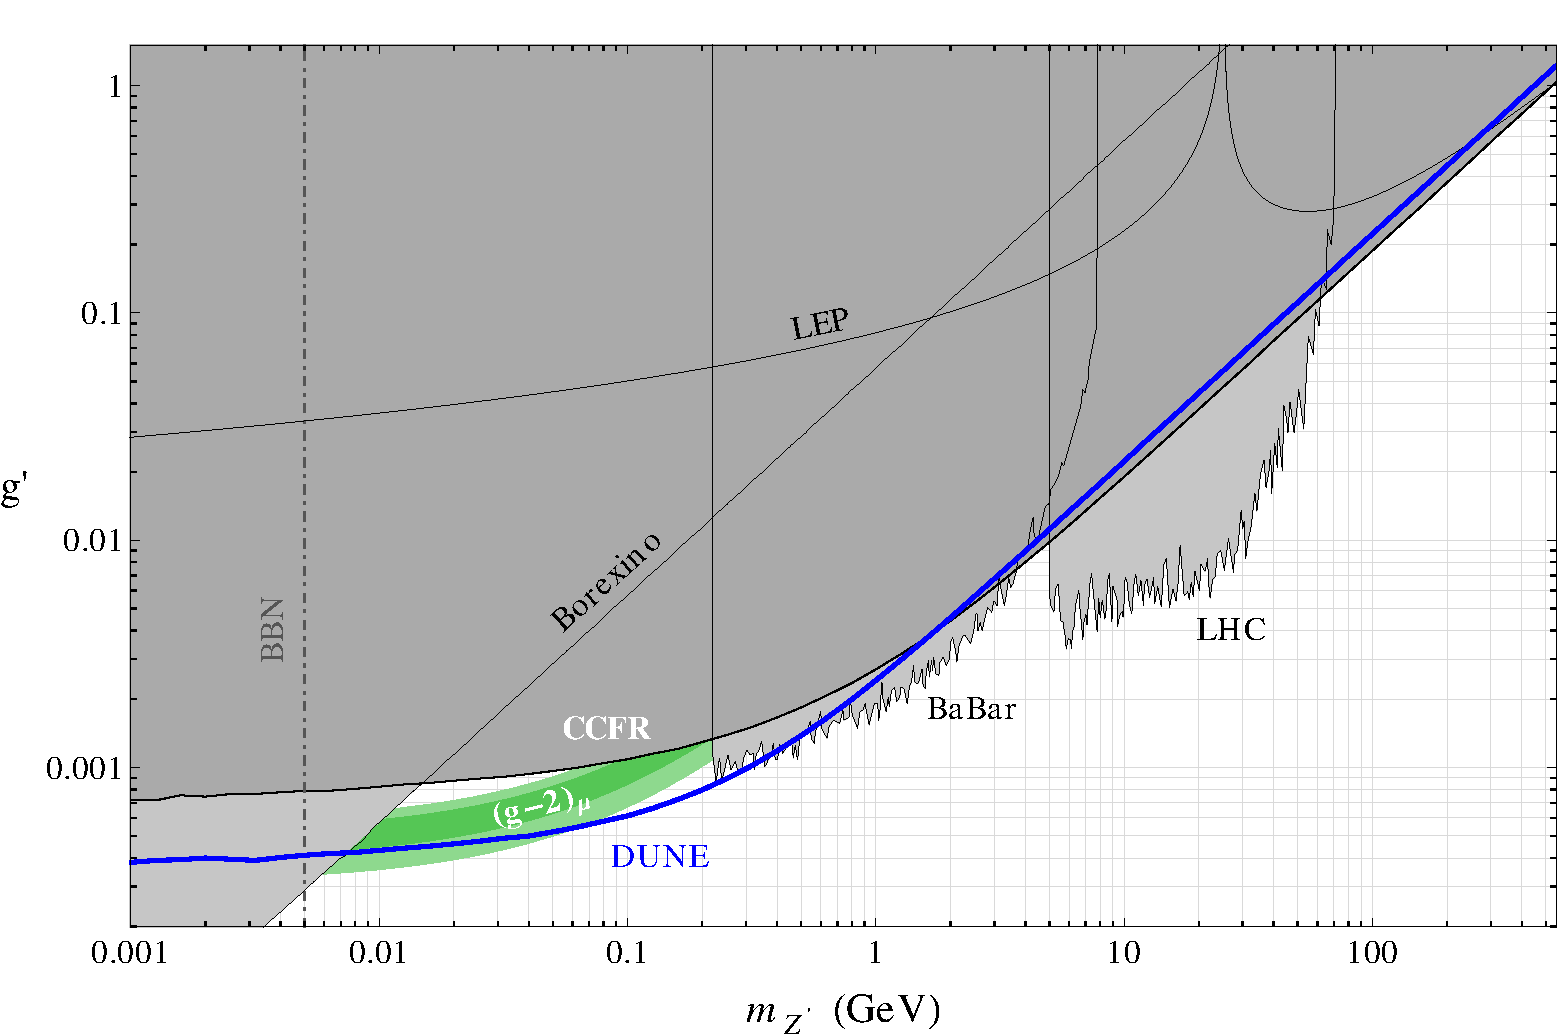
\includegraphics[width=0.55\textwidth]{LmuLtau.pdf}
\caption[Existing constraints and projected sensitivity in the $L_\mu - L_\tau$ parameter space]{Existing constraints and projected DUNE sensitivity in the $L_\mu - L_\tau$ parameter space. Shown in green is the region where the $(g-2)_\mu$ anomaly can be explained at the $2\sigma$ level. The parameter regions already excluded by existing constraints are shaded in gray and correspond to a CMS search for $pp \to \mu^+\mu^- Z' \to \mu^+\mu^-\mu^+\mu^-$~\cite{Sirunyan:2018nnz} (``LHC''), a BaBar search for $e^+e^- \to \mu^+\mu^- Z' \to \mu^+\mu^-\mu^+\mu^-$~\cite{TheBABAR:2016rlg} (``BaBar''), precision measurements of $Z \to \ell^+ \ell^-$ and $Z \to \nu\bar\nu$ couplings~\cite{ALEPH:2005ab,Altmannshofer:2014cfa} (``LEP''), a previous measurement of the trident cross section~\cite{Mishra:1991bv,Altmannshofer:2014pba} (``CCFR''), a measurement of the scattering rate of solar neutrinos on electrons~\cite{Bellini:2011rx,Harnik:2012ni,Agostini:2017ixy} (``Borexino''), and bounds from Big Bang Nucleosynthesis~\cite{Ahlgren:2013wba,Kamada:2015era} (``BBN''). The DUNE sensitivity shown by the solid blue line assumes a measurement of the trident cross section with $25\%$ precision.}
\label{fig:LmuLtau}
\end{figure}
%%%%%%%%%%%%%%%%%%%%%%%%%%%%%%%%%%%%%%%%%%%%%%%%%%%%%%%%%%%%%%%

In Figure~\ref{fig:LmuLtau} we show the existing CCFR constraint on the model parameter space in the $m_{Z'}$ vs. $g'$ plane and compare it to the region of parameter space where the anomaly in $(g-2)_\mu = 2 a_\mu$ can be explained. The green region shows the $1\sigma$ and $2\sigma$ preferred parameter space corresponding to a shift $\Delta a_\mu = a_\mu^\text{exp}-a_\mu^\text{SM} = (2.71 \pm 0.73) \times 10^{-9}$~\cite{Keshavarzi:2018mgv}.
Shown are in addition constraints from LHC searches for the $Z'$ in the $pp \to \mu^+\mu^- Z' \to \mu^+\mu^-\mu^+\mu^-$ process~\cite{Sirunyan:2018nnz} (see also~\cite{Altmannshofer:2014pba}), direct searches for the $Z'$ at BaBar using the $e^+e^- \to \mu^+\mu^- Z' \to \mu^+\mu^-\mu^+\mu^-$ process~\cite{TheBABAR:2016rlg}, and constraints from LEP precision measurements of leptonic $Z$ couplings~\cite{ALEPH:2005ab,Altmannshofer:2014cfa}.  
Also a Borexino bound on non-standard contributions to neutrino-electron scattering~\cite{Harnik:2012ni,Bellini:2011rx,Agostini:2017ixy} has been used to constrain the $L_\mu - L_\tau$ gauge boson~\cite{Kamada:2015era,Araki:2015mya,Kamada:2018zxi}. Our reproduction of the Borexino constraint is shown. 
For very light $Z'$ masses of $O$(few MeV) and below, strong constraints from measurements of the effective number of relativistic degrees of freedom during Big Bang Nucleosynthesis (BBN) apply~\cite{Ahlgren:2013wba,Kamada:2015era}.
Taking into account all relevant constraints, parameter space to explain $(g-2)_\mu$ is left below the di-muon threshold $m_{Z'} \lesssim 210$~MeV.

%%% NEUTRINO TRIDENTS %%%%%%%%%%%%%%%%%%%%%%%%%%%%%%%

%%%%%%%%%%%%%%%%%%%%%%%%%%%%%%%%%%%%%%%%
\section{Searches for NSI, Non-Unitarity, and \dword{cpt} Symmetry Violation}
%%%%%%%%%%%%%%%%%%%%%%%%%
\subsection{Non-Standard Interactions (NSI)}
\label{sec:nsi}
\dword{nsi} %Non-standard neutrino interactions 
can significantly modify the data to be collected by DUNE as long as the new physics parameters are large enough. \dword{nsi} may impact the determination of current unknowns such as \dword{cpv}~\cite{Masud:2015xva,Masud:2016bvp}, mass hierarchy~\cite{Masud:2016gcl} and octant of $\theta_{23}$~\cite{Agarwalla:2016fkh}. If the DUNE data are consistent with the standard oscillation for three massive neutrinos, \dword{nc} \dword{nsi}effects of order 0.1 $G_F$, affecting neutrino propagation through the Earth, can be ruled out at DUNE~\cite{deGouvea:2015ndi,Coloma:2015kiu}. We notice that DUNE might improve current constraints on $|\epsilon^m_{e \tau}|$ and $|\epsilon^m_{e \mu}|$ by a factor 2-5~\cite{Ohlsson:2012kf,Miranda:2015dra,Farzan:2017xzy}. New  \dword{cc}  interactions can also lead to modifications in the production and the detection of neutrinos. The findings on source and detector \dword{nsi} studies at DUNE are presented in~\cite{Blennow:2016etl,Bakhti:2016gic}. In particular, the simultaneous impact on the measurement of $\delta_{\rm CP}$ and $\theta_{23}$ is investigated in detail. Depending on the assumptions, such as the use of the \dword{nd}  and whether \dword{nsi} at production and detection are the same, the impact of source/detector \dword{nsi} at DUNE may be relevant. In this report we are assuming the results from~\cite{Blennow:2016etl} in which DUNE does not have sensitivity to discover or to improve bounds on source/detector \dword{nsi} to focus our attention in the propagation.

\subsubsection{NSI in propagation at DUNE}
%%%%%%%%%%%%%%%%%%%%%%%%%%%%%%%%%
%{\bf Authors: Chatterjee, Fernandez-Martinez, Forero, Guzzo, Kamiya, Miranda, Moura, Peres, Tortola, et al.}
\dword{nc} \dword{nsi} can be understood as non-standard
matter effects that are visible only in a \dword{fd} at a sufficiently long baseline. They can be parameterized as new contributions
to the \dword{msw} matrix in the neutrino-propagation Hamiltonian:
\begin{equation}
  H = U \left( \begin{array}{ccc}
           0 &                    & \\
             & \Delta m_{21}^2/2E & \\
             &                    & \Delta m_{31}^2/2E
         \end{array} \right) U^\dag + \tilde{V}_{\rm MSW} \,,
\end{equation}
with
\begin{equation}
  \tilde{V}_{\rm MSW} = \sqrt{2} G_F N_e
\left(
  \begin{array}{ccc}
    1 + \epsilon^m_{ee}       & \epsilon^m_{e\mu}       & \epsilon^m_{e\tau}  \\
        \epsilon^{m*}_{e\mu}  & \epsilon^m_{\mu\mu}     & \epsilon^m_{\mu\tau} \\
        \epsilon^{m*}_{e\tau} & \epsilon^{m*}_{\mu\tau} & \epsilon^m_{\tau\tau}
  \end{array} 
\right)
\label{eq:epsmatrix}
\end{equation}
Here, $U$ is the standard \dword{pmns} leptonic mixing matrix, for which we use the standard parameterization found, e.g., in~\cite{Agashe:2014kda}, and the $\epsilon$-parameters give the
magnitude of the \dword{nsi} relative to standard weak interactions.  For new physics
scales of a few hundred GeV,  a value of $|\epsilon|$ of the order
%%%\lesssim 
0.01 or less is
expected~\cite{Davidson:2003ha,GonzalezGarcia:2007ib,Biggio:2009nt}. DUNE
%%%\kmadj{1300} 
baseline provides an advantage in the detection of  \dword{nsi} relative
to existing beam-based experiments with shorter baselines.
Only atmospheric-neutrino experiments have longer baselines, but the sensitivity
of these experiments to  \dword{nsi} is limited by systematic effects~\cite{Adams:2013qkq}.

To assess DUNE sensitivity to \dword{nc}  \dword{nsi}, the  \dword{nsi} discovery reach
is defined in the following way: the expected event spectra are
simulated using  \dword{globes}~\cite{Huber:2004ka,Huber:2007ji}, assuming \textit{true} values for the  \dword{nsi} 
parameters, and a fit is then attempted assuming no  \dword{nsi}. If the fit is
incompatible with the simulated data at a given confidence level,
the chosen \emph{true} values of the  \dword{nsi} parameters are considered to be within the experimental discovery reach.

In this analysis, we use  \dword{globes} with the Monte Carlo Utility Based Experiment Simulator (MonteCUBES) C library~\cite{Blennow:2009pk}, a plugin that replaces the deterministic  \dword{globes} minimizer by a Markov Chain Monte Carlo (MCMC) method that is able to handle higher dimensional parameter spaces. In the simulations we use the configuration for the DUNE \dword{cdr}~\cite{Alion:2016uaj}. Each point scanned by the MCMC is stored and a frequentist $\chi^2$ analysis is performed with the results.

Considering that  \dword{nsi} exists, conducting the analysis with all the  \dword{nsi} parameters free to vary, we obtain the sensitivity regions in Figure~\ref{fig:nsi}. We omit the superscript $m$ that appears in eq.~\ref{eq:epsmatrix}. 
The credible regions are given in terms of percent \dword{cl}.
\begin{figure}[!htb]
	\centering
    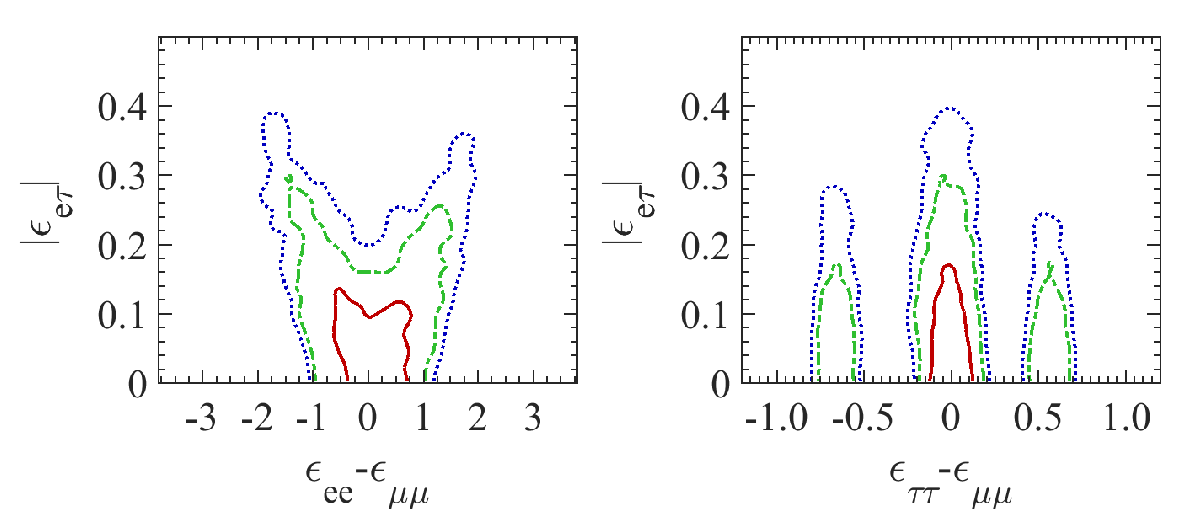
\includegraphics[width=0.6\columnwidth]{TDR12.pdf}
    
    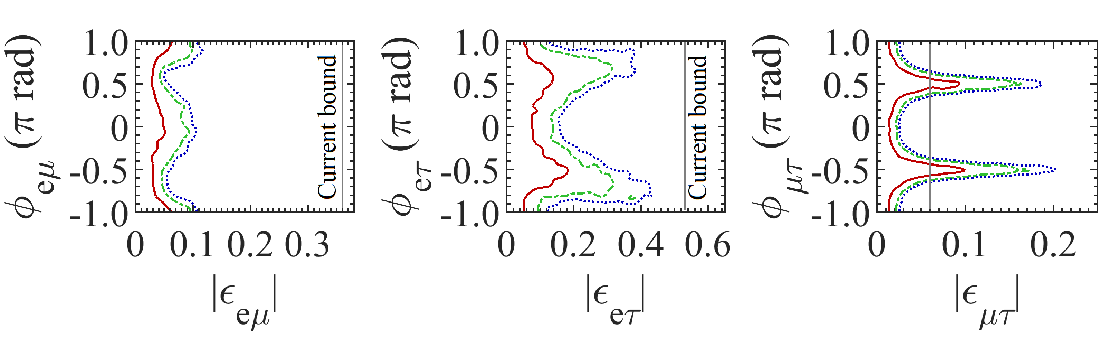
\includegraphics[width=0.75\columnwidth]{TDR4.pdf}
   \caption[NSI parameters. Allowed regions.]{\label{fig:nsi}Allowed regions of the non-standard oscillation parameters in which we see important degeneracies (top) and the complex non-diagonal ones (bottom). We conduct the analysis considering all the  \dword{nsi} parameters non-negligible. The sensitivity regions are for 68\% (red line (left)), 90\% (green dashed line (middle)), and 95\% CL (blue dotted line (right)). Current bounds are taken from~\cite{Gonzalez-Garcia:2013usa}.}
\end{figure}
We note, however, that constraints on $\epsilon_{\tau\tau}-\epsilon_{\mu\mu}$ coming from global fit analysis~\cite{Gonzalez-Garcia:2013usa,Miranda:2015dra,Farzan:2017xzy,Esteban:2018ppq} can remove the left and right solutions of $\epsilon_{\tau\tau}-\epsilon_{\mu\mu}$ in Figure~\ref{fig:nsi}.

In order to constrain the standard oscillation parameters when  \dword{nsi} are %is 
present, we use the fit for three neutrino mixing from~\cite{Gonzalez-Garcia:2013usa} and implement prior constraints to restrict the region sampled by the MCMC. The sampling of the parameter space is explained in~\cite{Coloma:2015kiu} and the priors that we use can be found in table~\ref{tab:priors1}.
\begin{table}[htb]
\caption{Oscillation parameters and priors implemented with the MCMC calculating Figure~\ref{fig:nsi}.} \label{tab:priors1}
\begin{center}
\begin{tabular}{cccc}
\hline
\hline
Parameter&Nominal&1$\sigma$ range ($\pm$)\\ 
\hline
$\theta_{12}$ &0.19$\pi~\textrm{rad}$&2.29\%\\
$\sin^2(2\theta_{13})$ &0.08470&0.00292\\
$\sin^2(2\theta_{23})$ &0.9860&0.0123\\
$\Delta m^2_{21} $ &7.5 $\times10^{-5}\textrm{eV}^2$&2.53\%\\
$\Delta m^2_{31} $ &2.524 $\times10^{-3}\textrm{eV}^2$&free\\
$\delta_{\rm CP} $ &1.45$\pi~\textrm{rad}$&free\\
\hline 
\hline
\end{tabular}
\end{center}
\end{table}

Then we can observe the effects of  \dword{nsi} on the measurements of the standard oscillation parameters at DUNE. In Figure~\ref{fig:standar-nsi}, we superpose the allowed regions with non-negligible  \dword{nsi} and the standard-only credible regions at 90\% \dword{cl}. %There is an important degeneracy that 
An important degeneracy appears in the measurement of the mixing angle $\theta_{23}$. We also see that the sensitivity of the \dword{cp} phase is strongly affected.
\begin{figure}[!htb]
	\centering
    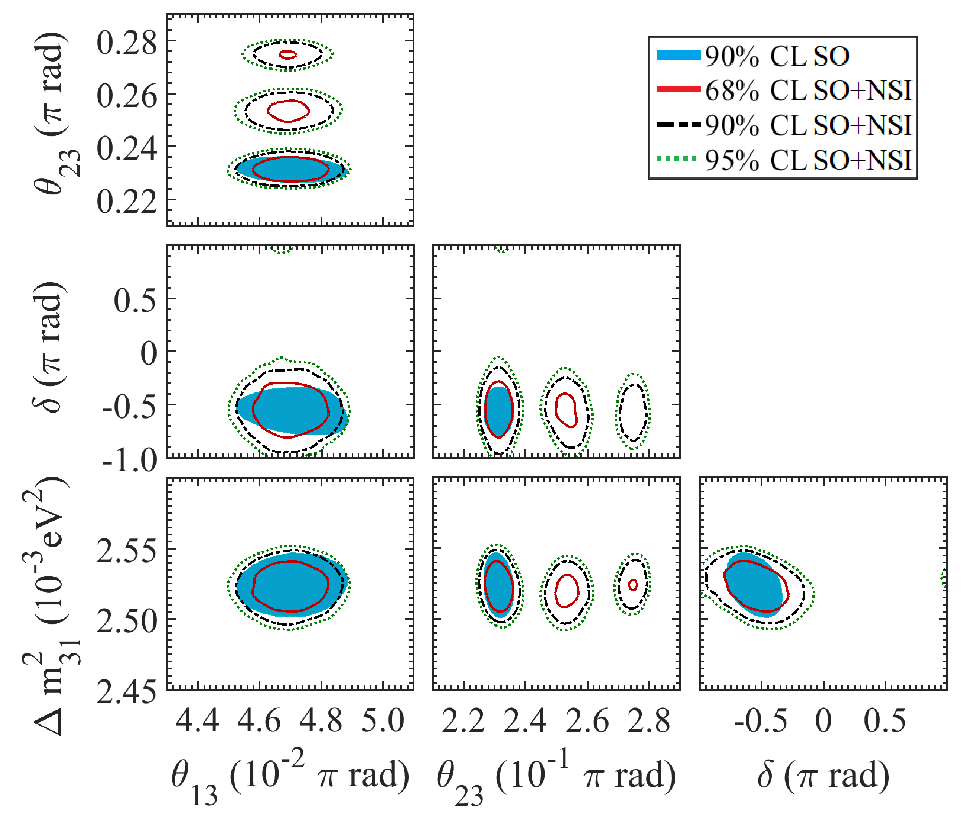
\includegraphics[width=0.6\columnwidth]{TDR10.pdf}
   \caption[Projections of the standard oscillation parameters considering  \dword{nsi} is possible]{\label{fig:standar-nsi}Projections of the standard oscillation parameters considering  \dword{nsi} is possible. The sensitivity regions are for 68\%, 90\%, and 95\% \dword{cl}. The allowed regions considering negligible  \dword{nsi} (standard oscillation (SO)) are superposed to the SO+NSI at 90\% \dword{cl}.}
\end{figure}

%%%%%%%%%%%%%%%%%%%%%%%%%%%%%%%%%%%%%%%%%%%%%%%%%%%%%%%%%%%%%%
\subsubsection{Effects of baseline and matter density variation on  \dword{nsi} measurements}\label{ssec:matter}
%%%%%%%%%%%%%%%%%%%%%%%%%%%%%%%%%%%%%%%%%%%%%%%%%%%%%%%%%%%%%%
The effects of matter density variation and its average along the beam path from \fnal to \surf  were studied considering the standard neutrino oscillation framework with three flavors~\cite{Roe:2017zdw,Kelly:2018kmb}. In order to obtain the results of Figures~\ref{fig:nsi} and~\ref{fig:standar-nsi}, we use a high-precision calculation for the baseline of \SI{1284.9}{km} and the average density of \SI{2.8482}{g/cm^3}~\cite{Roe:2017zdw}.

The DUNE collaboration has been using the so-called PREM~\cite{Dziewonski:1981xy,PREM2} density profile to consider matter density variation. With this assumption, the neutrino beam crosses a few constant density layers.
However, a more detailed density map is available for the USA with more than 50 layers and $0.25 \times 0.25$ degree cells of latitude and longitude: The Shen-Ritzwoller or S.R. profile~\cite{SR:2016,Roe:2017zdw}. Comparing the S.R. with the PREM profiles, Kelly and Parke~\cite{Kelly:2018kmb} show that, in the standard oscillation paradigm, DUNE is not highly sensitive to the density profile and that the only oscillation parameter with its measurement slightly impacted by the average density true value is \deltacp{}.
\dword{nsi}, however, may be sensitive to the profile, particularly considering the phase $\phi_{e\tau}$~\cite{Chatterjee:2018dyd}, to which DUNE will have a high sensitivity~\cite{Ohlsson:2012kf,Miranda:2015dra,deGouvea:2015ndi,Coloma:2015kiu,Farzan:2017xzy}, as we also see in Figure~\ref{fig:nsi}.

\subsubsection{Conclusions and prospects}
\dword{nsi} can significantly impact on the determination of current unknowns such as \dword{cpv} and the octant of $\theta_{23}$. Clean determination of the intrinsic \dword{cp} phase at long-baseline experiments such as DUNE is a formidable task~\cite{Rout:2017udo}. A feasible strategy to extricate physics scenarios at DUNE using high-energy beams was suggested in~\cite{Masud:2017bcf}.

%%%%%%%%%%%%%%%%%%%%%%%%%
\subsection{Non-Unitarity (NU)}
%{\bf Authors: Fernandez-Martinez, Forero, Miranda, Tórtola
%\vspace{0.5cm}
A generic characteristic of most models explaining the neutrino mass
pattern is the presence of heavy neutrino states, beyond the
three light states of the \dword{sm}  of particle
physics~\cite{Minkowski:1977sc,Mohapatra:1979ia,Yanagida:1979as,GellMann:1980vs}. This implies a deviation from unitarity of the $3\times3$ \dword{pmns} matrix, which can be particularly sizable %the lower the mass of the extra states are
as the mass of the extra states becomes lower~\cite{Mohapatra:1986bd,Akhmedov:1995vm,Akhmedov:1995ip,Malinsky:2005bi}.
For values of non-unitarity parameter deviations of order $10^{-2}$, this would decrease the expected reach of DUNE to the standard parameters, although stronger bounds existing from charged leptons would be able to restore its expected performance~\cite{Blennow:2016jkn,Escrihuela:2016ube}.

A generic characteristic of most models explaining the neutrino mass
pattern is the presence of heavy neutrino states, additional to the
three light states of the \dword{sm}  of particle
physics~\cite{Mohapatra:1998rq,Valle:2015pba,Fukugita:2003en}. These
types of models will imply that the $3 \times 3$ \dword{pmns} matrix is not
unitary due to the mixing with the additional states.  Besides the
type-I seesaw
mechanism~\cite{GellMann:1980vs,Yanagida:1979as,Mohapatra:1979ia,Schechter:1980gr},
different low-scale seesaw models include right-handed neutrinos that
are relatively not-so-heavy~\cite{Mohapatra:1986bd} and perhaps
detectable at collider experiments.

These additional heavy leptons would mix with the light neutrino
states and, as a result, the complete unitary mixing matrix will be \fixme{will or would?}
a
squared $n \times n$ matrix, with $n$ the total number of neutrino
states. As a result, the usual $3 \times 3$ \dword{pmns} matrix, which we dub $N$ to stress its non-standard nature, will be
non-unitary. One %of the possible general ways 
possible general way to parameterize these unitarity deviations in $N$ is through a triangular matrix~\cite{Escrihuela:2015wra}\footnote{For a similar parameterization corresponding to a $(3+1)$ and a $(3+3)$-dimensional mixing matrix,  see Refs.~\cite{Xing:2007zj,Xing:2011ur}}
%%
 \begin{equation}
  N = 
 \left\lgroup
 \begin{array}{ccc} 
 1-\alpha_{ee} & 0 & 0 \\
 \alpha_{\mu e} & 1-\alpha_{\mu \mu} & 0 \\
  \alpha_{\tau e} & \alpha_{\tau \mu} & 1-\alpha_{\tau \tau}
 \end{array}
 \right \rgroup U \,,
 \label{eq:triangular}
 \end{equation}
 % 
with $U$ a unitary matrix that tends to the usual \dword{pmns} matrix when the non-unitary parameters $\alpha_{ij} \rightarrow 0$\footnote{The original parameterization in Ref.~\cite{Escrihuela:2015wra} uses $\alpha_{ii}$ instead of $\alpha_{\beta\gamma}$. The equivalence between the two notations is as follows: $\alpha_{ii} = 1-\alpha_{\beta\beta}$ and $\alpha_{ij} = \alpha_{\beta\gamma}$.} .
%
 The triangular
matrix in this equation accounts for the non-unitarity of the $3 \times 3$ matrix for any number of extra neutrino species. This parametrization has been shown to be particularly well-suited for oscillation searches~\cite{Escrihuela:2015wra,Blennow:2016jkn} since, compared to other alternatives, it minimizes the departures of its unitary component $U$ from the mixing angles that are directly measured in neutrino oscillation experiments when unitarity is assumed.

The phenomenological implications of a non-unitary leptonic mixing matrix have been extensively studied in flavor and electroweak precision observables as well as in the neutrino oscillation phenomenon~\cite{Shrock:1980vy,Schechter:1980gr,Shrock:1980ct,Shrock:1981wq,Langacker:1988ur,Bilenky:1992wv,Nardi:1994iv,Tommasini:1995ii,Antusch:2006vwa,FernandezMartinez:2007ms,Antusch:2008tz,Biggio:2008in,Antusch:2009pm,Forero:2011pc,Alonso:2012ji,Antusch:2014woa,Abada:2015trh,Fernandez-Martinez:2015hxa,Escrihuela:2015wra,Parke:2015goa,Miranda:2016wdr,Fong:2016yyh,Escrihuela:2016ube}. For recent global fits to all flavor and electroweak precision data summarizing present bounds on non-unitarity see Refs.~\cite{Antusch:2014woa,Fernandez-Martinez:2016lgt}. 

%%%%%%%%%%%%%%%%%%%%%
\begin{table}[htb]
\caption[Expected $90 \%$~\dword{cl} constraints on the non-unitarity parameters $\alpha$]{\label{tab:bounds} Expected $90 \%$~\dword{cl}  constraints on the non-unitarity parameters $\alpha$ from DUNE. }
\begin{center}
\renewcommand{\arraystretch}{1.6}
\begin{tabular}{  l@{\quad\quad}  c@{\quad\quad}   c@{\quad\quad}   c@{\quad\quad}      }
\hline
$\alpha_{ee}$ & $0.3$ & $\alpha_{\mu e}$ & $0.04$  \\
$\alpha_{\mu\mu}$ & $0.2$ & $\alpha_{\tau e}$ & $0.7$ \\
$\alpha_{\tau\tau}$ & $0.8$ & $\alpha_{\tau\mu}$ & $0.2$  \\ \hline
\end{tabular}
\end{center}
\end{table}
%%%%%%%%%%%%%%%%%%%%%

\subsubsection{NU constraints from DUNE}
Recent studies have shown that DUNE can constrain the non-unitarity parameters~\cite{Blennow:2016jkn, Escrihuela:2016ube}. The summary of the $90 \%$~\dword{cl}  bounds on the different $\alpha_{ij}$ elements profiled over all other parameters is given in Table~\ref{tab:bounds}. 
These bounds are comparable with other constraints from present oscillation experiments, although they are not competitive with those obtained from flavor and electroweak precision data.
For this analysis, and %the ones that will be 
those presented below, we have used the  \dword{globes} software~\cite{Huber:2004ka,Huber:2007ji} with the DUNE \dword{cdr} configuration presented in Ref.~\cite{Alion:2016uaj}. The standard (unitary) oscillation parameters have also been treated as in~\cite{Alion:2016uaj}. The unitarity deviations have been included both by an independent code (used to obtain the results shown in Ref.~\cite{Escrihuela:2016ube}) and via the MonteCUBES~\cite{Blennow:2009pk} plug-in to cross validate our results.

\subsubsection{NU impact on DUNE standard searches}
Conversely, the presence of non-unitarity may affect the determination of the
Dirac \dword{cp}-violating phase $\delta_{CP}$ in long-baseline experiments~\cite{Miranda:2016wdr,Fernandez-Martinez:2016lgt,Escrihuela:2016ube}.
 Indeed, when allowing for unitarity deviations, the expected \dword{cp} discovery potential for DUNE could be significantly reduced.
However, the situation is alleviated when a combined analysis with the constraints on non-unitarity from other experiments is considered. This is illustrated in Figure~\ref{fig:CPsens}. In the left panel, the discovery potential for \dword{cpv} is computed when the non-unitarity parameters introduced in Eq.~(\ref{eq:triangular}) are allowed in the fit. While for the Asimov data all $\alpha_{ij}=0$, the non-unitary parameters are allowed to vary in the fit with $1 \sigma$ priors of $10^{-1}$, $10^{-2}$ and $10^{-3}$ for the dotted green, dashed blue and solid black lines respectively. For the dot-dashed red line no prior information on the non-unitarity parameters has been assumed. As can be observed, without additional priors on the non-unitarity parameters, the capabilities of DUNE to discover \dword{cpv} from $\delta_{CP}$ would be seriously compromised~\cite{Escrihuela:2016ube}. However, with priors of order $10^{-2}$ matching the present constraints from other neutrino oscillation experiments~\cite{Escrihuela:2016ube,Blennow:2016jkn}, the standard sensitivity is almost recovered. If the more stringent priors of order $10^{-3}$ stemming from flavor and electroweak precision observables are added~\cite{Antusch:2014woa,Fernandez-Martinez:2016lgt}, the standard sensitivity is obtained.   

The right panel of Figure~\ref{fig:CPsens} concentrates on the impact of the phase of the element $\alpha_{\mu e}$ in the discovery potential of \dword{cpv} from $\delta_{CP}$, since this element has a very important impact in the $\nu_e$ appearance channel. In this plot the modulus of $\alpha_{ee}$, $\alpha_{\mu \mu}$ and $\alpha_{\mu e}$ have been fixed to $10^{-1}$, $10^{-2}$, $10^{-3}$ and 0 for the dot-dashed red, dotted green, dashed blue and solid black lines respectively. All other non-unitarity parameters have been set to zero and the phase of $\alpha_{\mu e}$ has been allowed to vary both in the fit and in the Asimov data, showing the most conservative curve obtained. As for the right panel, it can be seen that a strong deterioration of the \dword{cp} discovery potential could be induced by the phase of $\alpha_{\mu e}$ (see Ref.~\cite{Escrihuela:2016ube}). However, for unitarity deviations of order $10^{-2}$, as required by present neutrino oscillation data constraints, the effect is not too significant in the range of $\delta_{CP}$ for which a $3 \sigma$ exclusion of \dword{cp} conservation would be possible and it becomes negligible if the stronger $10^{-3}$ constraints from flavor and electroweak precision data are taken into account.  

Similarly, the presence of non-unitarity worsens degeneracies involving $\theta_{23}$, making the determination of the octant or even its maximality challenging.
This situation is shown in Figure~\ref{fig:octant} where an input value of $\theta_{23} = 42.3^\circ$ was assumed. As can be seen, the fit in presence of non-unitarity (solid lines) introduces degeneracies for the wrong octant and even for maximal mixing~\cite{Blennow:2016jkn}. However, these degeneracies are solved upon the inclusion of present priors on the non-unitarity parameters from other oscillation data (dashed lines) and a clean determination of the standard oscillation parameters following DUNE expectations is again recovered.   

\begin{figure}[!t]
\centering
 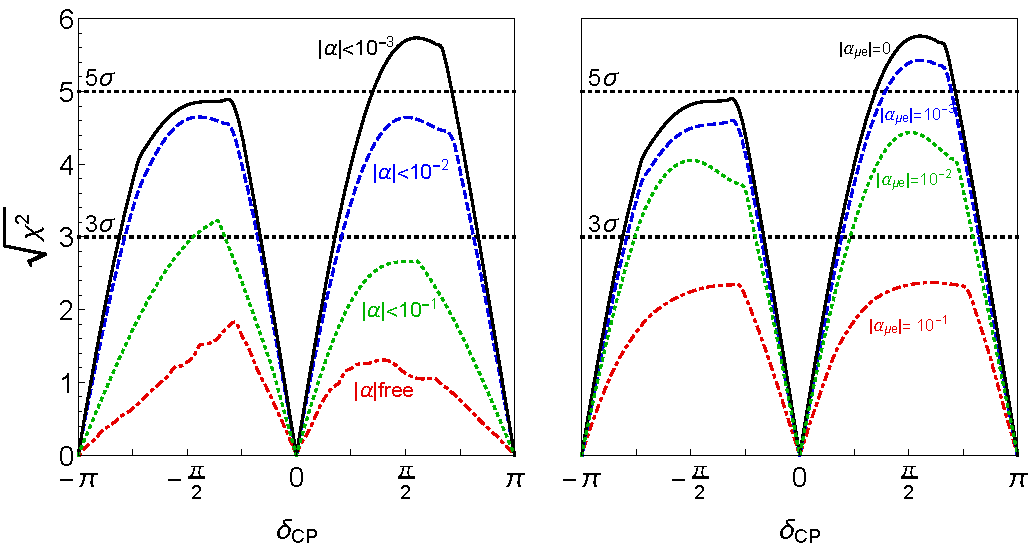
\includegraphics[width=0.8\columnwidth]{cpsens-comb.pdf}
\caption[Impact of non-unitarity on the \dword{cpv} discovery potential]{The impact of non-unitarity on the DUNE \dword{cpv} discovery potential. See the text for details.}
\label{fig:CPsens}
\end{figure}

\begin{figure}
 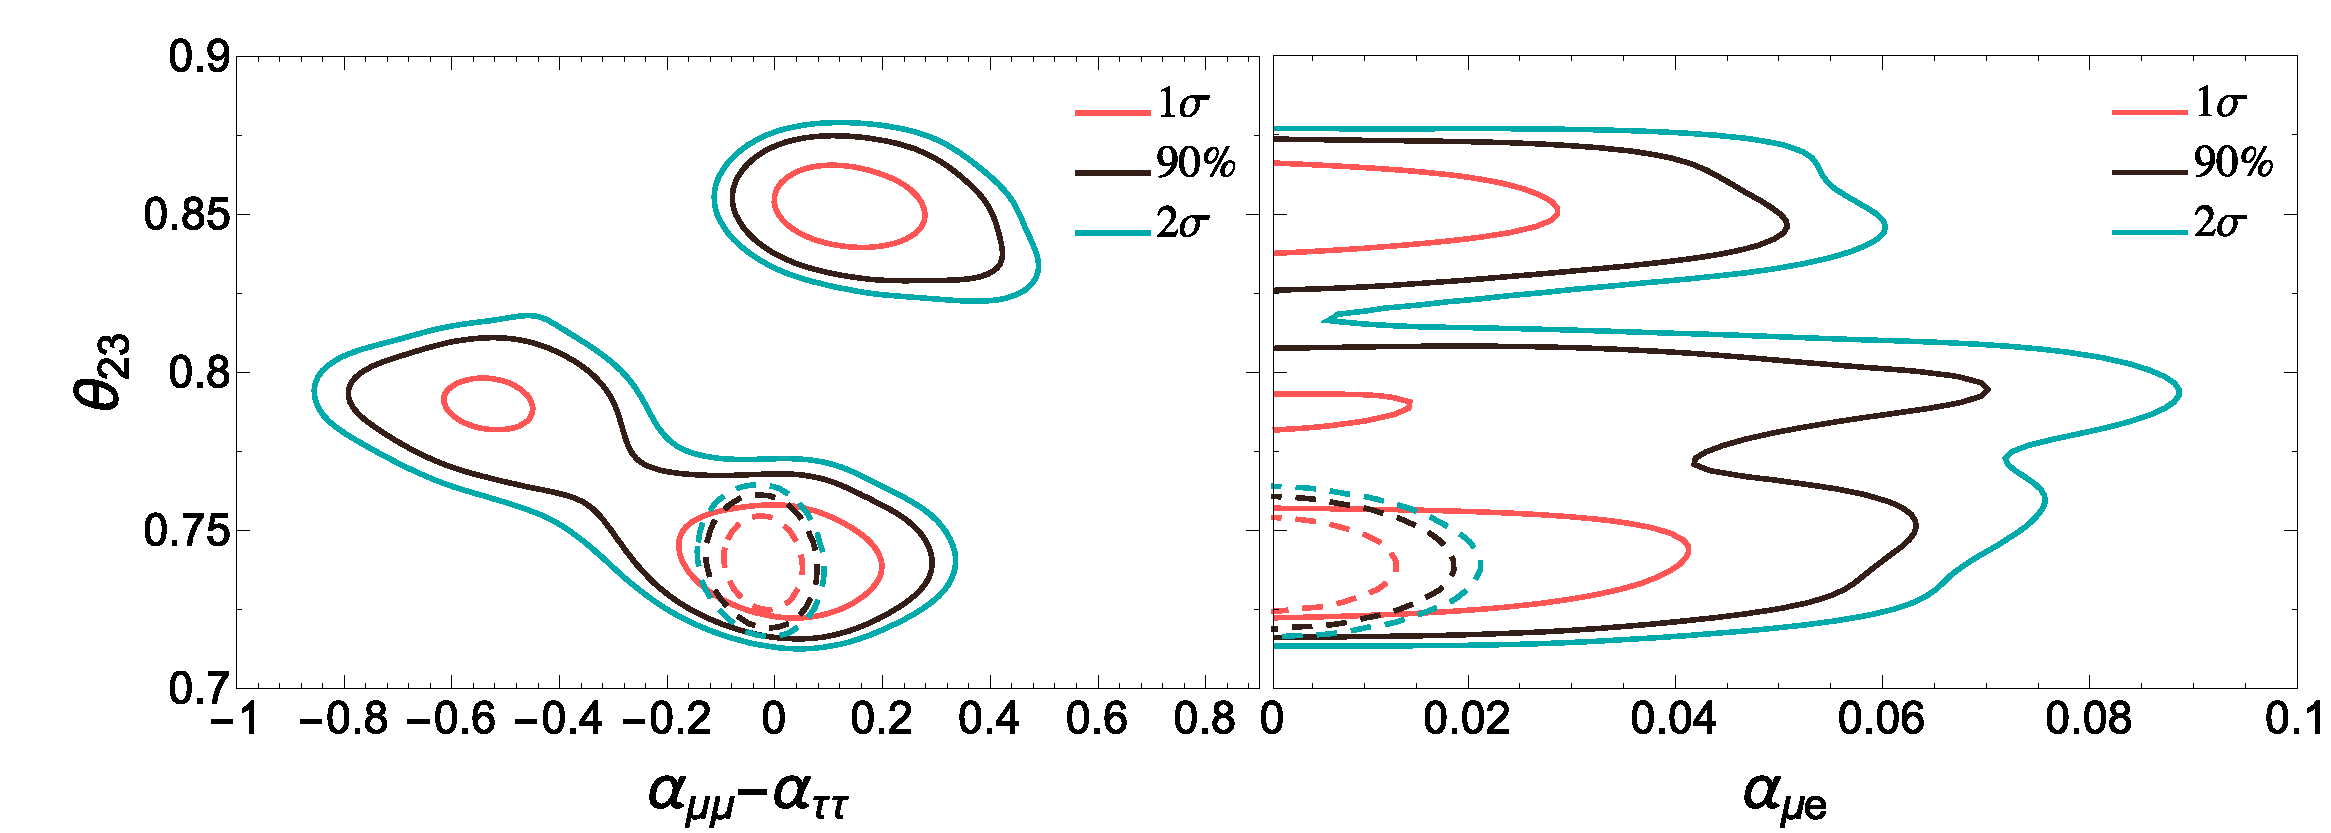
\includegraphics[width=0.8\columnwidth]{combined_pdf.pdf} 
 \begin{center}
  \caption[Expected frequentist allowed regions at the $1 \sigma$,
    $90\%$ and $2 \sigma$ CL\ ]{Expected frequentist allowed regions at the $1 \sigma$,
    $90\%$ and $2 \sigma$ CL\ for DUNE. All new physics parameters
    are assumed to be zero so as to obtain the expected
    non-unitarity sensitivities. The solid
    lines correspond to the analysis of DUNE data alone, while the
    dashed lines include the present constraints on non-unitarity.
\label{fig:octant}}
 \end{center}
\end{figure}

\subsubsection{Conclusions}
A non-unitary lepton mixing matrix, as generally expected from the most common extensions of the \dword{sm}  explaining neutrino masses, would affect the neutrino oscillations to be measured by DUNE. The sensitivity that DUNE would provide to the non-unitarity parameters is comparable to that from present oscillation experiments, while not competitive to that from flavor and electroweak precision observables, which is roughly an order of magnitude more stringent. Conversely, the capability of DUNE to determine the standard oscillation parameters such as \dword{cpv} from $\delta_{CP}$ or the octant or maximality of $\theta_{23}$ would be seriously compromised by unitarity deviations in the \dword{pmns}. This negative impact is however significantly reduced when priors on the size of these deviations from other oscillation experiments are considered and disappears altogether if the more stringent constraints from flavor and electroweak precision data are added instead.

%%%%%%%%%%%%%%%%%%%%%%%%%
\subsection{CPT Symmetry Violation}
%{\bf Authors: Barenboim, Ternes, and Tórtola.}

\dword{cpt} symmetry, the combination of charge conjugation, parity and time reversal, is a cornerstone of our model-building strategy. 
DUNE can improve the present limits on Lorentz and \dword{cpt} violation by several orders of magnitude~\cite{Streater:1989vi,Barenboim:2002tz,Kostelecky:2003cr,Diaz:2009qk,Kostelecky:2011gq,Barenboim:2017ewj}, contributing as a very important experiment to test one of the deepest results of quantum field theory.
%
\dword{cpt} invariance is surely one of the predictions of major importance of local, relativistic quantum field theory. One of the predictions of \dword{cpt} invariance is that particles and antiparticles have the same masses and, if unstable, the same lifetimes. To prove the \dword{cpt} theorem one needs only three ingredients~\cite{Streater:1989vi}: Lorentz invariance, hermiticity of the Hamiltonian, and locality.
%

Experimental bounds on \dword{cpt} invariance can be derived using the neutral kaon system~\cite{Schwingenheuer:1995uf}:
%
\begin{equation}
  \frac{|m(K^0) - m(\overline{K}^0)|}{m_K} < 0.6 \times 10^{-18}\,. 
  \label{eq:mK}
\end{equation}
%
This result, however, should be interpreted very carefully for two reasons. First, we do not have a complete theory of \dword{cpt} violation, and it is therefore rather arbitrary to take the kaon-mass as a scale. Second, since kaons are bosons, the term entering the Lagrangian is the mass squared and not the mass itself. With this in mind, we can rewrite the previous bound as:
%
%\begin{equation}
 $ |m^2(K^0) - m^2(\overline{K}^0)| < 0.3~\mbox{eV}^2 \, $.
%  \label{eq:mK2}
%\end{equation}
%
Here we %will 
see that neutrinos can test the predictions of the \dword{cpt} theorem to an unprecedented extent and could, therefore, provide stronger limits than the ones regarded as the most stringent ones %by now
to date\footnote{\dword{cpt} was tested also using charged leptons. However, these measurements involve a combination
of mass and charge and are not a direct \dword{cpt} test. Only neutrinos can provide \dword{cpt} tests on an elementary mass not contaminated by charge.}. 
%
In the absence of a solid model of flavor, not to mention one of \dword{cpt} violation, the spectrum  of neutrinos and antineutrinos can differ both  in the mass eigenstates themselves as well as in the flavor composition of each of these states. It is important to notice then that neutrino oscillation experiments can  only test \dword{cpt} in the mass differences and mixing angles. An overall shift between the neutrino and antineutrino spectra will be missed by oscillation experiments.  Nevertheless, such a pattern can be bounded by cosmological data~\cite{Barenboim:2017vlc}. Unfortunately direct searches for neutrino mass (past, present, and future) involve only antineutrinos and hence 
cannot be used to draw any conclusion on  \dword{cpt} invariance on the absolute mass scale,  either.
%
Therefore, using neutrino oscillation data, we will compare the mass splittings and mixing angles of  neutrinos with those of antineutrinos. Differences in the neutrino and antineutrino spectrum would imply the violation of the \dword{cpt} theorem.

In Ref.~\cite{Barenboim:2017ewj} the authors derived the most up-to-date bounds on \dword{cpt} invariance from the neutrino sector %. The data used to derive these bounds are the same considered in the global fit to neutrino oscillations in Ref.~\cite{deSalas:2017kay}. 
using the same data that was used in the global fit to neutrino oscillations in Ref.~\cite{deSalas:2017kay}. 
Of course, experiments that cannot distinguish between neutrinos and antineutrinos, such as atmospheric data from \superk~\cite{Abe:2017aap}, IceCube-DeepCore~\cite{Aartsen:2014yll,Aartsen:2017nmd} and ANTARES~\cite{AdrianMartinez:2012ph} were not included. The complete data set used, as well as the parameters to which they are sensitive, are % the following:
%
%\begin{itemize}
 (1) from solar neutrino data~\cite{Cleveland:1998nv,Kaether:2010ag,Abdurashitov:2009tn,hosaka:2005um,Cravens:2008aa,Abe:2010hy,Nakano:PhD,Aharmim:2008kc,Aharmim:2009gd,Bellini:2013lnn}:  $\theta_{12}$, $\Delta m_{21}^2$, and $\theta_{13}$;
 (2) from neutrino mode in long-baseline experiments K2K~\cite{Ahn:2006zza}, MINOS~\cite{Adamson:2013whj,Adamson:2014vgd}, T2K~\cite{Abe:2017uxa,Abe:2017bay}, and NO$\nu$A~\cite{Adamson:2017qqn,Adamson:2017gxd}:  $\theta_{23}$, $\Delta m_{31}^2$, and $\theta_{13}$;
 (3) from KamLAND reactor antineutrino data~\cite{Gando:2010aa}: $\overline{\theta}_{12}$, $\Delta \overline{m}_{21}^2$, and $\overline{\theta}_{13}$;
 (4) from short-baseline reactor antineutrino experiments Daya Bay~\cite{An:2016ses}, RENO~\cite{RENO:2015ksa}, and Double Chooz~\cite{Abe:2014bwa}:     $\overline{\theta}_{13}$ and $\Delta \overline{m}_{31}^2$; and 
 (5) from antineutrino mode in long-baseline experiments MINOS~\cite{Adamson:2013whj,Adamson:2014vgd} and T2K~\cite{Abe:2017uxa,Abe:2017bay}: $\overline{\theta}_{23}$, $\Delta \overline{m}_{31}^2$, and
$\overline{\theta}_{13}$\footnote{The K2K experiment took  data only in neutrino mode, while the \nova experiment has not published data in the antineutrino mode yet.}. %\\
%\end{itemize}

From the analysis of all previous data samples, one can derive the most up-to-date bounds on \dword{cpt} violation:
%
% \begin{eqnarray}
$ |\Delta m_{21}^2-\Delta \overline{m}_{21}^2| < 4.7\times 10^{-5} \,  \text{eV}^2,\,\,
%  \nonumber \\
 |\Delta m_{31}^2-\Delta \overline{m}_{31}^2| < 3.7\times 10^{-4} \, \text{eV}^2,\,\,
% \nonumber \\
 |\sin^2\theta_{12}-\sin^2\overline{\theta}_{12}| < 0.14\,,\,\,
%  \\
 |\sin^2\theta_{13}-\sin^2\overline{\theta}_{13}| < 0.03\,, \,\,
%  \nonumber \\
 {\rm and}~|\sin^2\theta_{23}-\sin^2\overline{\theta}_{23}| < 0.32\,.
 $  %\\
 %\nonumber.
% \label{eq:new-bounds}
% \end{eqnarray} 

At the moment it is not possible to set any bound on $|\delta-\overline{\delta}|$, since all possible values of
$\delta$ or $\overline{\delta}$ are allowed by data. The preferred intervals of $\delta$ obtained in Ref.~\cite{deSalas:2017kay} can only be obtained after combining the neutrino and antineutrino data samples. 
The limits  on $\Delta(\Delta m_{31}^2)$ and $\Delta(\Delta m_{21}^2)$  are already better than the one derived from the neutral kaon system and should be regarded as the best current bounds on \dword{cpt} violation on the mass squared. % so far. 
Note that these results were derived assuming the same mass ordering for neutrinos and antineutrinos. If the ordering was different for neutrinos and antineutrinos, this would be an indication for \dword{cpt} violation on its own. In the following we show how DUNE could improve this bound.

\subsubsection{Sensitivity to \dword{cpt} symmetry violation in the neutrino sector}
\label{sec:sensitivity}

\begin{table}[htb]\centering
%  \catcode`?=\active \def?{\hphantom{0}}
\caption[Oscillation parameters used to simulate neutrino and antineutrino data]{Oscillation parameters used to simulate neutrino and antineutrino data analyzed in Section~\ref{sec:sensitivity}.}
     \label{tab:par2}
   \begin{tabular}{lc}
    \hline
    parameter & value 
    \\
    \hline
    $\Delta m^2_{21}$& $7.56\times 10^{-5}\text{eV}^2$\\  
    %%
    $\Delta m^2_{31}$&  $2.55\times 10^{-3}\text{eV}^2$\\
    %%	
    $\sin^2\theta_{12}$ & 0.321\\ 
     $\sin^2\theta_{23}$ &  0.43, 0.50, 0.60\\
    $\sin^2\theta_{13}$ & 0.02155\\
   $\delta$ & 1.50$\pi$\\
       \hline
 
     \end{tabular}
%       \captionsetup{justification=centering}
\end{table}

Here we study the sensitivity of the DUNE experiment to measure \dword{cpt} violation in the neutrino sector by analyzing neutrino and antineutrino oscillation parameters separately. We assume the neutrino oscillations being parameterized by the usual \dword{pmns} matrix $U_{\text{PMNS}}$, with parameters $\theta_{12},\theta_{13},\theta_{23},\Delta m_{21}^2,\Delta m_{31}^2, {\rm and}~\delta$, while the antineutrino oscillations are parameterized by a matrix $\overline{U}_{\text{PMNS}}$ with parameters $\overline{\theta}_{12},\overline{\theta}_{13},\overline{\theta}_{23},\Delta \overline{m}_{21}^2,\Delta \overline{m}_{31}^2, {\rm and}~\overline{\delta}$. Hence, antineutrino oscillation is described  by the same probability functions as neutrinos with the neutrino parameters replaced by their antineutrino counterparts\footnote{Note that the antineutrino oscillation probabilities also include the standard change of sign in the \dword{cp} phase.}. 
To simulate the future neutrino data signal in DUNE, in this section we assume the true values for neutrinos and antineutrinos to be as listed %the ones 
in Table~\ref{tab:par2}.
Then, in the statistical analysis, we vary freely all the oscillation parameters, except the solar ones, which are fixed to their best fit values throughout the simulations. Given the great precision in the determination of the reactor mixing angle by the short-baseline reactor experiments~\cite{An:2016ses,RENO:2015ksa,Abe:2014bwa}, in our analysis we use a prior on $\overline{\theta}_{13}$, but not on $\theta_{13}$. We also consider three different values for the atmospheric angles, as indicated in Table~\ref{tab:par2}. 

Therefore, to test the sensitivity at DUNE we perform the simulations assuming $\Delta x = |x-\overline{x}| = 0$, where $x$ is any of the oscillation parameters. Then we estimate the sensitivity to $\Delta x\neq 0$. To do so we calculate two $\chi^2$-grids, one for neutrinos and one for antineutrinos, varying the four parameters of interest. After minimizing over all parameters except $x$ and $\overline{x}$, we calculate 
%
\begin{equation}
 \chi^2(\Delta x) = \chi^2(|x-\overline{x}|) = \chi^2(x)+\chi^2(\overline{x}),
 \label{eq:chi2-nu-nubar}
\end{equation}
%
where we have considered all the possible combinations of $|x-\overline{x}|$. The results are presented in Figure~\ref{fig:sensitivity-CPT}, where we plot three different lines, labelled as ``high'', ``max'' and ``low.'' These refer to the assumed value for the atmospheric angle: in the lower octant (low), maximal mixing (max) or in the upper octant (high). Here we can see that there is sensitivity neither to $\Delta(\sin^2\theta_{13})$, where the 3$\sigma$ bound would be of the same order %of 
as the current measured value for $\sin^2\overline{\theta}_{13}$, nor to $\Delta\delta$, where no single value of the parameter would be excluded at more than 2$\sigma$.

On the contrary, interesting results for $\Delta(\Delta m_{31}^2)$ and $\Delta(\sin^2\theta_{23})$ are obtained. First, we see that  DUNE can put stronger bounds on the difference of the atmospheric mass splittings, namely $\Delta(\Delta m_{31}^2) < 8.1\times 10^{-5}$, improving the current neutrino bound by one order of magnitude. For the atmospheric angle, we obtain different results depending on the true value assumed in the simulation of DUNE data. In the lower right panel of Figure~\ref{fig:sensitivity-CPT} we see the different behavior obtained for $\theta_{23}$ lying in the lower octant, being maximal and lying in the upper octant. 
\fixme{clarify previous sentence. (anne)} As one might expect, the sensitivity increases with $\Delta\sin^2\theta_{23}$ in the case of maximal mixing. However, if the true value lies in the lower or upper octant, a degenerate solution appears in the complementary octant.
\begin{figure}[!htb]
 \centering
        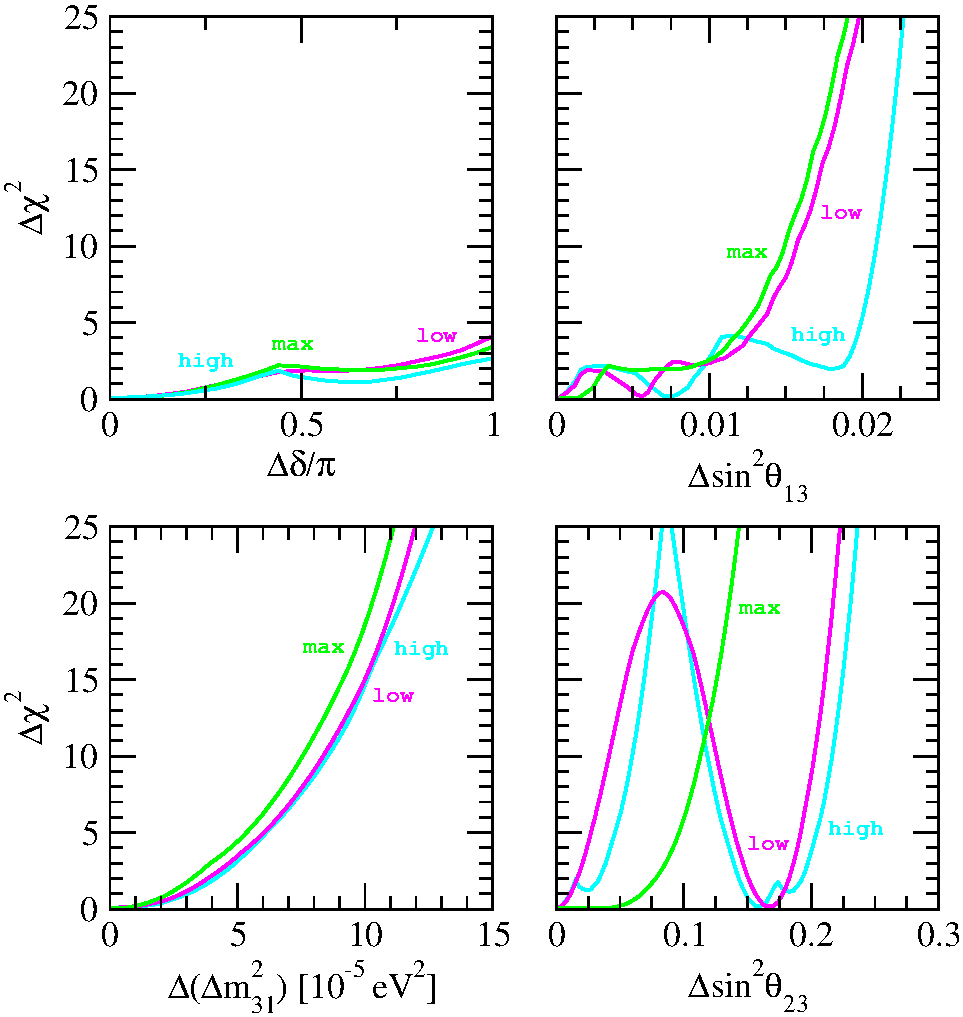
\includegraphics[width=0.55\columnwidth]{sensitivity-CPT.pdf}
        \caption[Sensitivities to the difference of neutrino and antineutrino parameters]{The sensitivities of DUNE to the difference of neutrino and antineutrino parameters: 
        $\Delta\delta$, $\Delta(\Delta m_{31}^2)$, $\Delta(\sin^2\theta_{13})$ and $\Delta(\sin^2\theta_{23})$  
        for the atmospheric angle in the lower octant (magenta line),  in the upper octant (cyan line) and for maximal mixing (green line).}
	\label{fig:sensitivity-CPT}
\end{figure}

\subsubsection{Imposter solutions}
\label{sec:impost}
In %different 
some types of neutrino oscillation experiments, e.g., accelerator experiments, neutrino and antineutrino data are obtained in separate experimental runs. The usual procedure followed by the experimental collaborations, as well as the global oscillation fits as for example Ref.~\cite{deSalas:2017kay}, assumes \dword{cpt} invariance and analyzes the full data sample in a joint way. \fixme{I'm trying to parse this. Is this right? ``Experimental collaborations usually assume \dword{cpt} invariance and analyze the full data sample in a holistic way. Global oscillation fits, e.g., by~\cite{deSalas:2017kay}, are usually done following a similar procedure.'' }
However, if \dword{cpt} is violated in nature, the outcome of the joint data analysis might give rise to what we call an ``imposter'' solution, i.e., %a solution that results from the combined analysis but 
one that does not correspond to the true solution of any channel. 

Under the assumption of \dword{cpt} conservation, the $\chi^2$ functions are computed according to
%
\begin{equation}
 \chi^2_{\text{total}}=\chi^2(\nu)+\chi^2(\overline{\nu})\, ,
 \label{eq:CPT-cons}
\end{equation}
%
and assuming that the same parameters describe neutrino and antineutrino flavor oscillations. In contrast, in Eq.~(\ref{eq:chi2-nu-nubar}) we first profiled over the parameters in neutrino and antineutrino mode separately and then added the profiles. Here, we shall assume \dword{cpt} to be violated in nature, but perform our analysis as if it were conserved. As an example, we assume that the true value for the atmospheric neutrino mixing is $\sin^2\theta_{23}=0.5$, while the antineutrino mixing angle is given by $\sin^2\overline{\theta}_{23}=0.43$. The rest of the oscillation parameters are set to the values in Table~\ref{tab:par2}. Performing the statistical analysis in the \dword{cpt}-conserving way, as indicated in Eq.~(\ref{eq:CPT-cons}), we obtain the profile of the atmospheric mixing angle presented in Figure~\ref{fig:imposter-sq23}. The profiles for the individual reconstructed results (neutrino and antineutrino) are also shown in the figure for comparison.
%As can be seen, we obtain
The result is a new best fit value at $\sin^2\theta^\text{comb}_{23}=0.467$, disfavoring the true values for neutrino and antineutrino parameters at approximately 3$\sigma$ and more than 5$\sigma$, respectively. 

\begin{figure}[!htb]
 \centering
        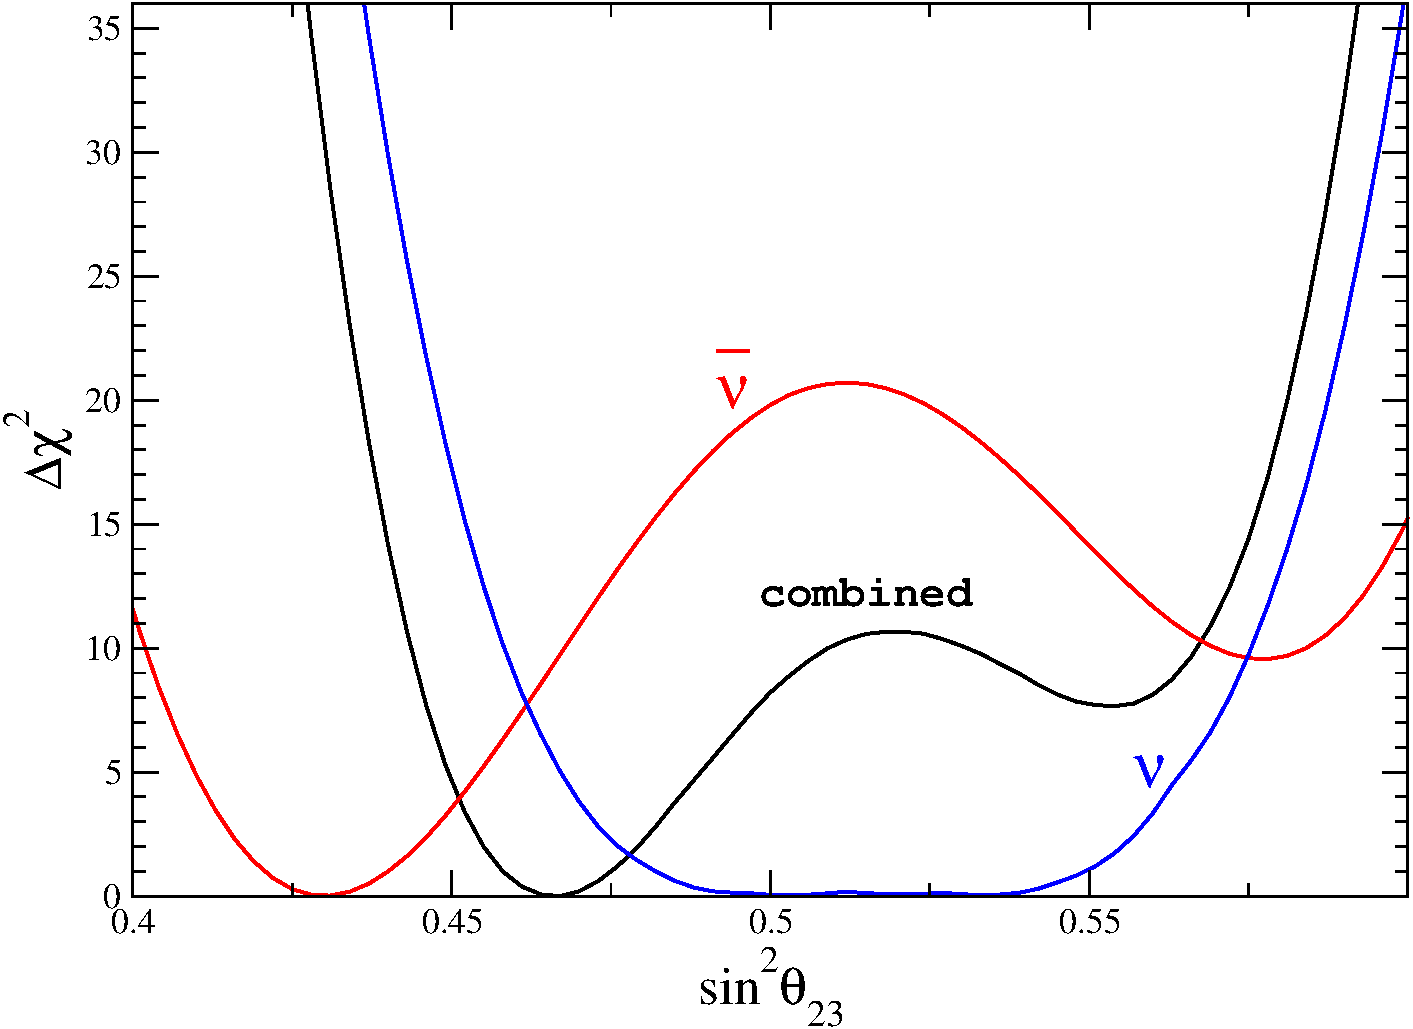
\includegraphics[width=0.6\columnwidth]{imposter-sq23.pdf}
        \caption[Sensitivity to atmospheric angle for neutrinos, antineutrinos, and combination under \dword{cpt} conservation]{DUNE sensitivity to the atmospheric angle for neutrinos (blue), antineutrinos (red) and to the combination of both under the assumption of \dword{cpt} conservation (black).
         }
	\label{fig:imposter-sq23}
\end{figure}

%%%%%%%%%%%%%%%%%%%%%%%%%%%%%%%%%%%%%%%%
\section{Search for Boosted Dark Matter from the Sun}

%%%%%%%%%%%%%%%%%%%%%%%%%
\subsection{\label{sec:level1}Introduction}

Due to the increasingly stronger constraints on the longstanding paradigm of \dword{dm}, \dwords{wimp}, it is of utmost importance to expand the \dword{dm} searches to include alternative candidates and non-minimal scenarios. A class of models called \dword{bdm} was first studied in~\cite{Huang:2013xfa,Agashe:2014yua, Berger:2014sqa}, leading to the novel phenomenology that a small non-thermal component of \dword{dm} today is relativistic and effectively interacts with \dword{sm} particles, which could %can 
be the smoking-gun for \dword{dm} discovery. This is in contrast to the conventional assumption that \dword{dm} is composed of one particle species that is deeply non-relativistic. \dword{bdm} originates from \dword{dm} annihilation in a two-component dark sector or semi-annihilation in the original work, but can also generically arise from other scenarios~\cite{Carlson:1992fn, Hochberg:2014dra,Huang:2013xfa}. 

Conventional \dword{dm} direct detection is generally not suitable to capture the small flux of \dword{bdm} that leads to energetic outgoing \dword{sm} particles upon its scattering (for an  exception, see~\cite{Cherry:2015oca, Cui:2017ytb}). On the other hand, large-volume neutrino detectors stand out as natural, ideal facilities for such searches. The two interaction channels of \dword{bdm}, with electrons~\cite{Agashe:2014yua} and with hadrons (protons)~\cite{Berger:2014sqa}, were investigated for Cherenkov detectors, such as \superk, which recently published a dedicated search for \dword{bdm} in the electron channel~\cite{Kachulis:2017nci}. However, in such detectors the \dword{bdm} signal rate is shown to  often be significantly attenuated due to Cherenkov threshold, in particular for hadronic channels. 

The recently developed \lar detectors, such as DUNE's, have the potential to greatly improve the sensitivity for \dword{bdm} compared to Cherenkov detectors. This is due to improved particle identification techniques, as well as a significantly lower energy threshold for proton detection. Earlier studies have shown an improvement with DUNE for \dword{bdm}-electron interaction \cite{Necib:2016aez}. In this work that uses %employing 
newly developed dedicated simulation tools, we demonstrate that DUNE can %majorly 
significantly expand the reach of \superk when \dword{bdm} scatters off protons.

Other studies of \dword{bdm} models have examined sensitivity at DUNE and elsewhere~\cite{Agashe:2014yua,Berger:2014sqa,Alhazmi:2016qcs,Necib:2016aez,Kim:2016zjx,Kachulis:2017nci,Giudice:2017zke,Chatterjee:2018mej,Kim:2018veo}. The hadronic interaction model presented here is complementary to other model studies. This study is the first to study such a model at DUNE with full event generation and detector simulation.
\fixme{prev sentences are a bit awkward. Maybe: The hadronic interaction model study presented here is complementary to others, and is  the first for DUNE with full event generation and detector simulation.}

%%%%%%%%%%%%%%%%%%%%%%%%%
\subsection{\label{sec:level2}Theory Discussion}
In the remainder of this study, we focus on the example of \dword{bdm} arising from a two-component dark sector as studied in \cite{Agashe:2014yua, Berger:2014sqa}. This scenario consists of two stable dark particles, $\psi$ and $\chi$, specified as fermions. % in this study.
 Particle $\psi$ is more massive than $\chi$, and is the dominant \dword{dm} today with its abundance determined by thermal annihilation of $\psi\psi\rightarrow\chi\chi$. The present-day annihilation of $\psi$ leads to \dword{bdm} $\chi$ with a boost factor of $\gamma = m_\psi/m_\chi$. The \dword{bdm}-\dword{sm} interaction may proceed via exchange of a dark photon $\gamma'$ or $Z'$.

In this work we focus on \dword{bdm} flux sourced by \dword{dm} annihilation in the core of the sun. \dword{dm} particles can be captured by the sun through their scattering with the nuclei in the sun, mostly hydrogen and helium. This makes the core of the sun a region with concentrated \dword{dm} distribution. The \dword{bdm} flux is
\begin{eqnarray} \label{eq:flux}
\Phi= f \frac{A}{4\pi D^2},
\end{eqnarray}
where $A$ is the annihilation rate, and $D = 1\,\rm{AU}$ is the distance from the sun. $f$ is a model-dependent parameter, where $f = 2$ for two-component \dword{dm} as considered here.

For the parameter space of interest, %we are interested in, 
assuming that the 
\dword{dm} annihilation cross section is not too small, the \dword{dm} distribution in the sun has reached an equilibrium between capture and annihilation. This helps to eliminate the annihilation cross section dependence in our study.

Two additional comments are in order. First, the \dword{dm} particles cannot be too light, i.e.,  lighter than 4\,GeV~\cite{Griest:1986yu,Gould:1987ju}, otherwise we will lose most of the captured \dword{dm} through evaporation rather than annihilation; this would dramatically reduce the \dword{bdm} flux. Additionally, one needs to check that \dword{bdm} particles cannot lose energy and potentially be recaptured by scattering with the solar material when they escape from the core region after production. Rescattering is found to be rare for the benchmark models considered in this study and we consider the \dword{bdm} flux to be monochromatic at its production energy.

The event rate to be observed at DUNE is 
\begin{equation}
R = \Phi \times \sigma_{\rm{SM} - \chi} \times \epsilon \times N,
\end{equation}
 where $\Phi$ is the flux given by Eq. \ref{eq:flux}, $\sigma_{\rm{SM} - \chi}$ is the scattering cross section of the \dword{bdm} off of \dword{sm} particles, $\epsilon$ is the efficiency of the detection of such a process, and $N$ is the number of target particles in DUNE. The computation of the flux of \dword{bdm} from the sun can be found in~\cite{Berger:2014sqa}. 
 
We generate the signal events and calculate interaction cross sections in the detector using a newly developed \dword{bdm} module~\cite{Andreopoulos:2009rq,Andreopoulos:2015wxa,Berger:2018} that includes elastic and deep inelastic scattering, as well as a range of nuclear effects. This conservative event generation neglects the dominant contributions from baryon resonances in the final state hadronic invariant mass range of 1.2 to 1.8 GeV, which should not have a major effect on our main results. The interactions are taken to be mediated by an axial, flavor universal 
\fixme{is `flavor universal' a term that nodifies Zprime? I.e., flavor-universal?}
$Z^\prime$ coupling to both the \dword{bdm} and with the quarks. The axial charge is taken to be 1. 
% The resulting cross-sections with argon are shown in Tab.~\ref{tab:eff-tab}. 
The events are generated for the \nominalmodsize DUNE detector module~\cite{dunetpc_code}, though we only study the dominant scattering off of the \argon40 atoms therein. The method for determining the efficiency $\epsilon$ is described below. The number of target argon atoms is $N = 1.5  \times 10^{32}$ assuming a target mass of \nominalmodsize{}.

% -------------------------------------------------------------------------------
\subsection{Background Estimation}
\label{sec:background}

The main background in this process comes from the \dword{nc} 
interactions of atmospheric neutrinos and argon,
as they share the features that the timing of events is unknown in advance,
and that the interactions with argon produce hadronic activity in the detector.
We use \dword{genie}~cite{Andreopoulos:2009rq,Andreopoulos:2015wxa}
interfaced by the \dword{larsoft} toolkit to generate the \dword{nc} atmospheric
neutrino events, and obtain 845 events in a \nominalmodsize{} module for one year of
exposure.

%%%%%%%%%%%%%%%%%%%%%%%%%
\subsection{Detector Response}
\label{sec:detector_resp}

The finite detector resolution is taken into
account by smearing the direction of the stable final state particles, 
including protons, neutrons, charged pions, muons, electrons, and photons,
with the expected angular resolution,
and by ignoring the ones with kinetic energy below detector threshold,
using the parameters reported in the DUNE \dword{cdr}~\cite{DUNE_CDR_V2}.
We form as the observable the total momentum from all the stable final state particles,
and obtain its angle with respect to the direction of the sun.
The sun position is simulated with the SolTrack package~\cite{SolTrack}
including the geographical coordinates of the DUNE \dword{fd}~\cite{DUNE_DocDB136}.
We consider both the scenarios in which we can reconstruct neutrons and in which 
neutrons will not be reconstructed.
Figure~\ref{fig:m10_SmearedReconstructableAngle} shows the angular distributions of
the \dword{bdm} signals with mass of 10\,GeV and different boost factors,
and of the background events.

% ---------------------------------------------------------------------------------
\begin{figure*}[!htb]
\centering
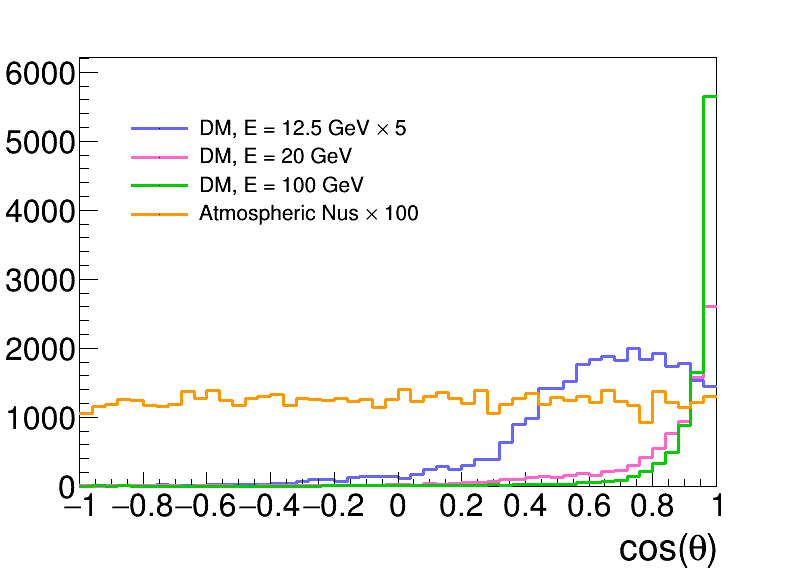
\includegraphics[width=0.45\textwidth]{m10_SmearedReconstructableAngle.png}
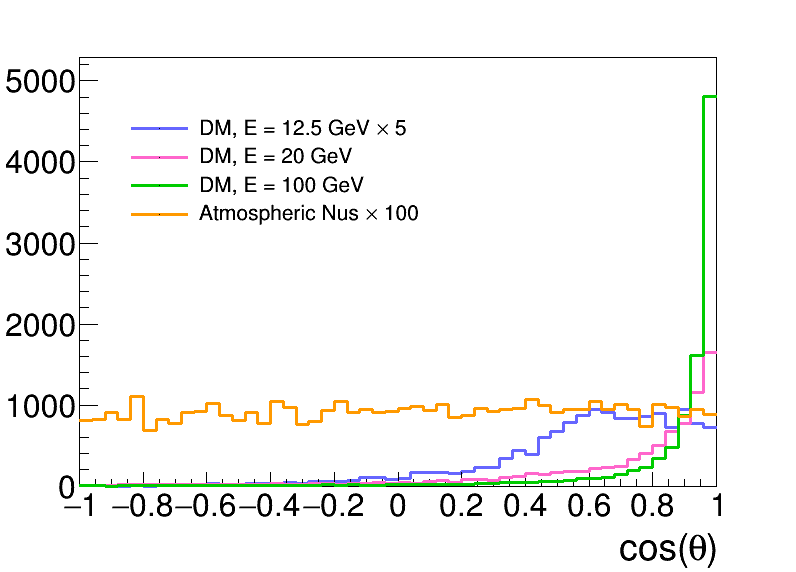
\includegraphics[width=0.45\textwidth]{m10_SmearedReconstructableNoNAngle.png}
\caption[Angular distribution of the \dword{bdm} signal events with the \dword{bdm} mass of 10\,GeV]{Angular distribution of the \dword{bdm} signal events with the \dword{bdm} mass of 10\,GeV
and different boosted factors, $\gamma$, and of the atmospheric neutrino NC
background events.
$\theta$ represents the angle of the sum over all the stable final state
particles as detailed in the text.
The amount of background represents one-year data collection, magnified by a factor 100,
while the amount of signal reflects the detection efficiency of 10,000 \dword{mc} events, as
described in this note.
The left plot shows the scenario where neutrons can be reconstructed,
while the right plot represents the scenario without neutrons.}
\label{fig:m10_SmearedReconstructableAngle}
\end{figure*}
% ---------------------------------------------------------------------------------


To increase the signal fraction in our samples, we select events with $\cos\theta > 0.6$,
and obtain the selection efficiency $\epsilon$ for different \dword{bdm} models.
% as listed in Table~\ref{tab:eff-tab}, 
$104.0 \pm 0.7$ and $79.4 \pm 0.6$ background events per year, in the scenarios with and without neutrons respectively,
survive the selection in a DUNE \nominalmodsize module.

%%%%%%%%%%%%%%%%%%%%%%%%%
\subsection{Results}

\begin{figure*}[!htb]
\centering
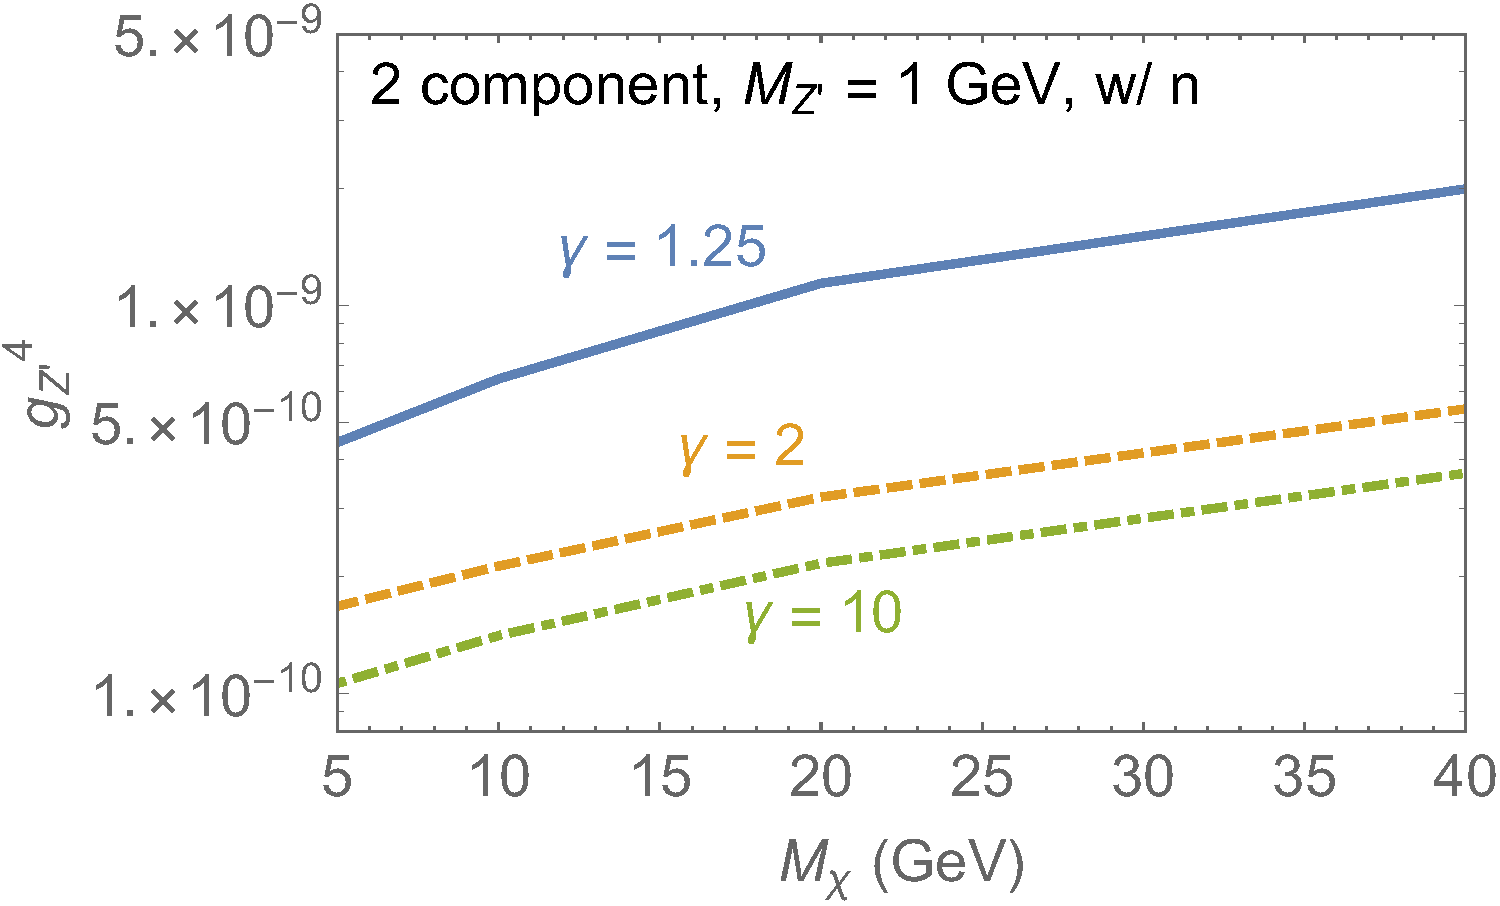
\includegraphics[width=0.45\textwidth]{expected-discovery-with-n.pdf}\hspace{0.05\textwidth}
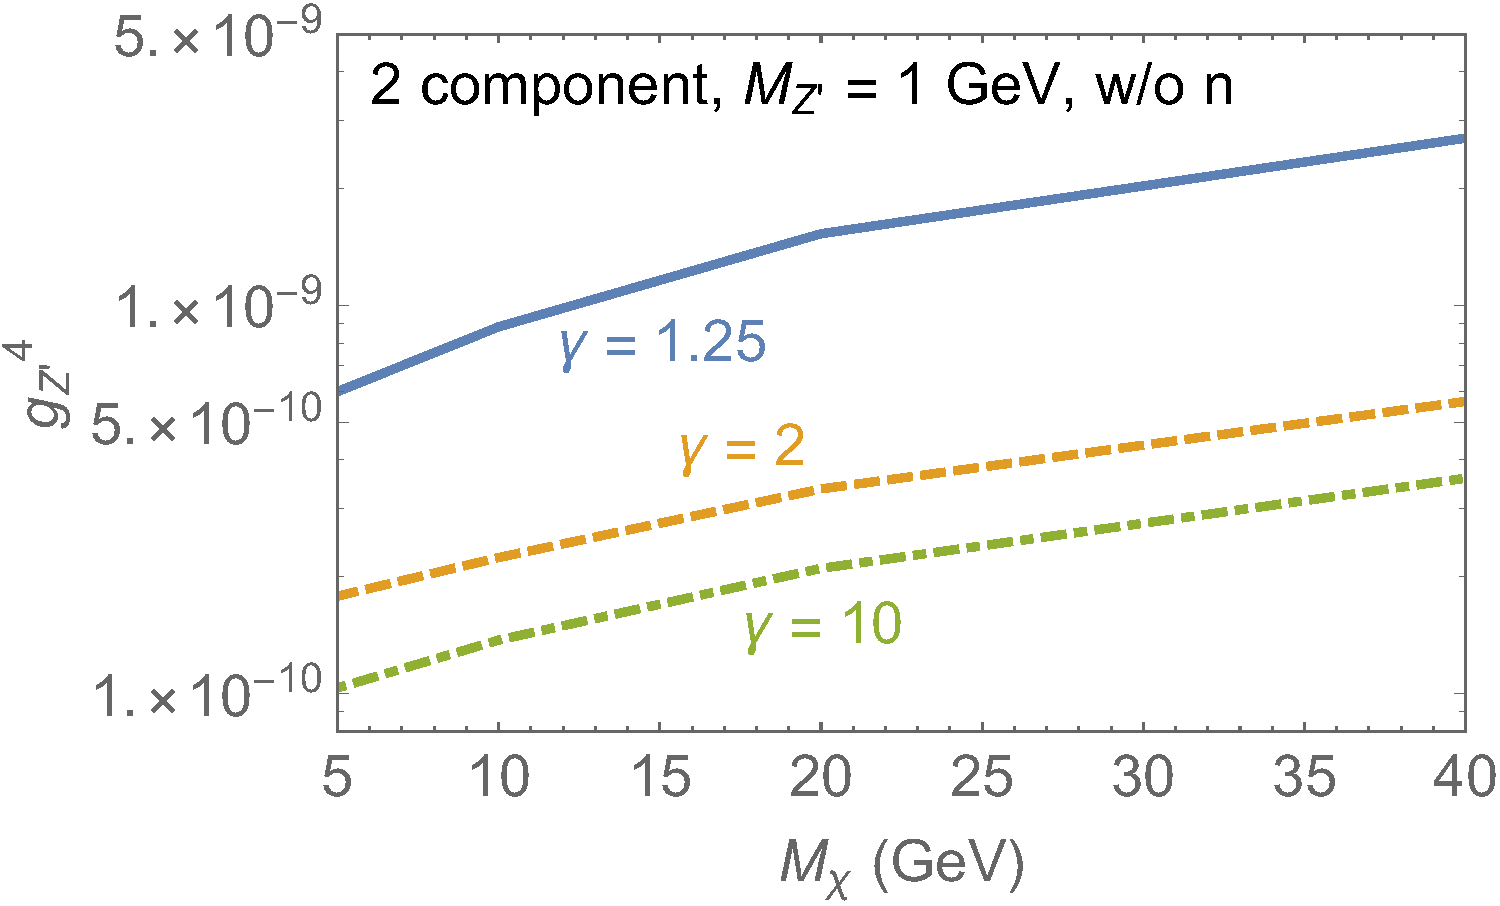
\includegraphics[width=0.45\textwidth]{expected-discovery-no-n.pdf}
\caption[Expected $5\sigma$ discovery reach with one year of DUNE livetime]{Expected $5\sigma$ discovery reach with one year of DUNE livetime including neutrons in reconstruction (left) and excluding neutrons (right).\label{fig:significance}}
\end{figure*}
The resulting expected sensitivity is presented in Figure~\ref{fig:significance} in terms of the \dword{dm} mass and the $Z^\prime$ gauge coupling for potential \dword{dm} boosts of $\gamma = 1.25,2,10$ and for a fixed mediator mass of $m_{Z^\prime} = 1~{\rm GeV}$.  We assume a DUNE livetime of one year.  The models presented here are currently unconstrained by direct detection searches if the thermal relic abundance of the \dword{dm} is chosen to fit current observations.

%%%%%%%%%%%%%%%%%%%%%%%%%
\subsection{Conclusions}

\dword{bdm} is motivated by a variety of non-minimal dark sector scenarios that has %gained
generated increasing interest in recent years. Thanks to its relatively low threshold and strong particle identification capabilities, DUNE presents an opportunity to significantly advance the search for  \dword{bdm} beyond what has been possible with water Cherenkov detectors. With one year of data, the $5\sigma$ sensitivity is expected to reach a coupling of $g_{Z^\prime}^4 = 9.57 \times 10^{-10}$ for a boost of 1.25 and $g_{Z^\prime}^4 = 1.49 \times 10^{-10}$ for a boost of 10 at a \dword{dm} mass of \SI{10}{GeV} without including neutrons in the reconstruction.


%%%%%%%%%%%%%%%%%%%%%%%%%%%%%%%%%%%%%%%%
\section{Other \dword{bsm} Physics Opportunities}

%%%%%%%%%%%%%%%%%%%%%%%%%
\subsection{Tau Neutrino Appearance} 

The tau neutrino was not directly observed until 2000 by the DONuT experiment, which used emulsion technology to detect  $\nu_{\tau}$-\dword{cc} and $\bar{\nu}_{\tau}$-\dword{cc} produced by $D_S$ meson decays originating from an \SI{800}{GeV} proton beam stopped by a tungsten alloy beam dump.  A total of nine $\nu_{\tau}$-\dword{cc} and $\bar{\nu}_{\tau}$-\dword{cc} candidate events were observed with an estimated background of 1.5 events~\cite{Kodama:2000mp, Kodama:2007aa}.

The OPERA experiment was also designed with emulsion technology to discover tau neutrino appearance in a muon neutrino beam~\cite{Guler:2000bd}. OPERA succeeded in discovering tau neutrino appearance~\cite{Agafonova:2015jxn}; however, the baseline and energy of the experiment was such that appearance was suppressed by a factor of 0.01.   The final analysis identified 10 $\nu_{\tau}$-\dword{cc} candidate events with an estimated background of two  events.  From this sample, a 20\% measurement of $\Delta m^{2}_{32}$ was performed under the assumption that $\sin^22\theta_{23} = 1$~\cite{Agafonova:2018auq}.  \superk has developed a method to statistically separate a sample of $\nu_{\tau}$-\dword{cc} and $\bar{\nu}_{\tau}$-\dword{cc} events in atmospheric neutrinos to exclude the no-tau-neutrino appearance hypothesis at the 4.6$\sigma$ level~\cite{Abe:2012jj, Li:2017dbe}, but limitations of water Cherenkov detectors limit the ability to select a high-purity sample and perform precision measurements.

With only 19 $\nu_{\tau}$-\dword{cc} and $\bar{\nu}_{\tau}$-\dword{cc} candidates detected with high purity, we have less direct experimental knowledge of tau neutrinos than any other \dword{sm}  particle. Our knowledge of the tau-neutrino cross-section is inferred from measurements of muon neutrinos assuming lepton universality, such that any cross section differences are only due to the large mass of the tau lepton. However, recent data from Belle, BaBar, and LHCb, as combined by the Heavy Flavor Averaging Group, 
\fixme{who is this group?}
shows that certain decays involving tau leptons differ from \dword{sm}  predictions assuming lepton universality by 3.9$\sigma$~\cite{Amhis:2016xyh}.  This anomaly could be explained with a $W'$-boson~\cite{Greljo:2018ogz}, which could potentially induce  \dword{nsi} affecting $\nu_{\tau}$ appearance.  Similarly, almost all knowledge of the tau-neutrino mixing-matrix elements comes from assuming unitarity of the mixing matrix. Without assuming unitarity, one critical element is only known to 60\%~\cite{Parke:2015goa}.

The DUNE experiment has the possibility of significantly improving the experimental situation.  Tau-neutrino appearance can potentially improve the discovery potential for sterile neutrinos, \dword{nc} \dword{nsi}, and non-unitarity.  For model independence, the first goal should be measuring the atmospheric oscillation parameters in the $\nu_{\tau}$ appearance channel and checking the consistency of this measurement with those performed using the $\nu_{\mu}$ disappearance channel.  A truth-level study of $\nu_{\tau}$ selection in atmospheric neutrinos in a large, underground LArTPC detector suggested that $\nu_{\tau}$-\dword{cc} interactions with hadronically decaying $\tau$-leptons, which make up 65\% of total $\tau$-lepton decays~\cite{PDG}, can be selected with high purity~\cite{Conrad:1008}.  This analysis suggests that it may be possible to select up to 29\% of $\nu_{\tau}$-\dword{cc} events with hadronically decaying $\tau$-leptons with minimal neutral current background.  Under these assumptions, we expect to select $\sim$25 $\nu_{\tau}$-\dword{cc} candidates per year using the \dword{cpv} optimized beam.  This is sufficient to %be able to 
simultaneously constrain $\Delta m^2_{31}$ and $\sin^22\theta_{23}$; however, all of these events occur at energies higher than the first oscillation maximum due to kinematic constraints.  Only seeing the tail of the oscillation maximum creates a partial degeneracy between the measurement of  $\Delta m^2_{31}$ and $\sin^22\theta_{23}$.  Atmospheric neutrinos, due to sampling a much larger $L/E$ range, allow for measuring both above and below the first oscillation maximum with $\nu_{\tau}$ appearance.  Although  we only expect to select $\sim$70 $\nu_{\tau}$-\dword{cc} and $\bar{\nu}_{\tau}$-\dword{cc} candidates in 350 kt-year in the atmospheric sample,  a direct measurement of the oscillation maximum should break the degeneracy seen in the beam sample.  Finally, a high-energy beam option optimized for $\nu_{\tau}$ appearance should produce $\sim$150 selected  $\nu_{\tau}$-\dword{cc} candidates in one year.  These higher energy events are further in the tail of the first oscillation maximum, but they will permit a simultaneous measurement of the $\nu_{\tau}$ cross section. 

%%%%%%%%%%%%%%%%%%%%%%%%%
\subsection{Heavy Neutral Leptons}
The high intensity of the LBNF neutrino beam and the production of charm and bottom mesons in the beam enables DUNE to search for a wide variety of lightweight long-lived, exotic particles, by looking for topologies of rare event interactions and decays in the fiducial volume of the DUNE \dword{nd} . These particles include weakly interacting heavy neutral leptons, such as right-handed partners of the active neutrinos, vector, scalar, or axion portals to the Hidden Sector, \fixme{undefined} 
and light super-symmetric particles. Assuming these heavy neutral leptons are the lighter particles of their hidden sector, they will only decay into \dword{sm}  particles. The parameter space explored by the DUNE \dword{nd}  extends into the cosmologically relevant region complementary to the LHC heavy-mass dark-matter searches through missing energy and mono-jets.

%%%%%%%%%%%%%%%%%%%%%%%%%
\subsection{Large Extra Dimensions}
DUNE can search for or constrain the size of large extra-dimensions %(LED) 
by looking for distortions of the oscillation pattern predicted by the three-flavor paradigm. These distortions arise through mixing between the right-handed neutrino Kaluza-Klein modes, which propagate in the compactified extra dimensions, and the active neutrinos, which exist only in the four-dimensional brane [48]. Searching for these distortions in, for instance, the $\nu_\mu$~\dword{cc} disappearance spectrum, should provide significantly enhanced sensitivity over existing results from the MINOS/MINOS+ experiment [49].

%%%%%%%%%%%%%%%%%%%%%%%%%
\subsection{Dark Matter Annihilation in the Sun}
DUNE's large \dword{fd} LArTPC modules provide an excellent setting to conduct searches for neutrinos arising from \dword{dm} annihilation in the core of the sun. These would typically result in a high-energy neutrino signal almost always accompanied by a low-energy neutrino component, which has its origin in a hadronic cascade that
develops in the dense solar medium and produces large numbers of light long-lived mesons, such as $\pi^+$ and $K^+$ that %, which will 
then stop and decay at rest. The decay of each $\pi^+$ and $K^+$ will
produce monoenergetic neutrinos with an energy \SI{30}{MeV} or \SI{236}{MeV}, respectively.
The  \SI{236}{MeV} flux can be measured with the DUNE \dword{fd}, thanks to its excellent energy resolution, and importantly, will benefit from directional information. By selecting neutrinos arriving from the direction of the sun, large reduction in backgrounds can be achieved.
This directional resolution for sub-GeV neutrinos will enable DUNE to be competitive with experiments with even larger fiducial masses, but less precise angular information, such as Hyper-K~\cite{ref:DMannihilation}.

%%%%%%%%%%%%%%%%%%%%%%%%%%%%%%%%%%%%%%%%
\section{Conclusions and Outlook}
DUNE will be a powerful discovery tool on a variety of physics topics under very active exploration today, from the potential discovery of new particules beyond those predicted in the \dword{sm}, to precision neutrino measurements that may uncover deviations from the present three-flavor mixing paradigm and unveil new interactions and symmetries.
The \dword{nd} alone will offer excellent opportunities to search for light \dword{dm} and mixing with light sterile neutrinos, and to measure rare processes such as neutrino trident interactions. Besides looking for deviations from the three-flavor oscillation paradigm such as nonstandard interaction, DUNE's massive high-resolution \dword{fd} will probe  the possible existence of \dword{bdm}. The flexibility of the LBNF beamline enables planning for high-energy beam running, providing access to probing and measuring tau neutrino physics with unprecedented precision.

DUNE will offer a long-term privileged setting for collaboration between experimentalists and theorists in the domain areas of neutrino physics, astrophysics, and cosmology, and will provide the highest potential for breakthrough discoveries among the new near-term facilities projected to start operations during the next decade.
